\documentclass[aspectratio=169, 10pt]{beamer}
\usepackage[utf8]{inputenc}
\usepackage[T1]{fontenc}
\usepackage{tikz}
\usepackage{booktabs}
\usepackage{graphicx}
\usepackage{tcolorbox}
\usepackage{colortbl}
\usepackage{amsmath}
\usepackage{xcolor}
\usetikzlibrary{calc, positioning, shadows, patterns, decorations.pathmorphing}

% ==========================================
% VIBRANT ORIGINAL DESIGN: MIDNIGHT & AMBER
% ==========================================
\definecolor{Midnight}{HTML}{0F172A}
\definecolor{VibrantAmber}{HTML}{F59E0B}
\definecolor{SoftMint}{HTML}{ECFDF5}
\definecolor{EmeraldEdge}{HTML}{10B981}
\definecolor{SlateText}{HTML}{1E293B}
\definecolor{RoseGold}{HTML}{FB7185}

\setbeamercolor{background canvas}{bg=white}
\setbeamercolor{normal text}{fg=SlateText}
\setbeamercolor{itemize item}{fg=VibrantAmber}
\setbeamertemplate{navigation symbols}{}

% CUSTOM DOODLE: HEARTBEAT
\newcommand{\heartbeatdoodle}[1]{
    \begin{tikzpicture}[#1]
        \draw[RoseGold, line width=1.5pt, cap=round, join=round] 
        (0,0) -- (0.2,0) -- (0.3,0.5) -- (0.4,-0.5) -- (0.5,1.2) -- (0.6,-0.8) -- (0.7,0) -- (1,0);
    \end{tikzpicture}
}

% CUSTOM DOODLE: DATA WAVE
\newcommand{\datawavedoodle}[1]{
    \begin{tikzpicture}[#1]
        \draw[EmeraldEdge, line width=1pt, opacity=0.4] 
        plot [smooth, tension=1] coordinates {(0,0) (0.5,0.3) (1,-0.2) (1.5,0.5) (2,0)};
    \end{tikzpicture}
}

% Header Template
\setbeamertemplate{frametitle}{
    \nointerlineskip
    \begin{beamercolorbox}[wd=\paperwidth,ht=1.4cm,dp=0.4cm]{frametitle}
        \begin{tikzpicture}[remember picture, overlay]
            \fill[Midnight] (current page.north west) rectangle ($(current page.north east) - (0, 1.4)$);
            % Original Geometric Doodle
            \fill[VibrantAmber] ($(current page.north east) - (2.5, 0)$) -- ($(current page.north east) - (1.5, 1.4)$) -- (current page.north east) -- cycle;
            \draw[VibrantAmber, line width=3pt] ($(current page.north west) + (0, -1.4)$) -- ($(current page.north east) + (0, -1.4)$);
            \node[anchor=west, white, font=\Large\bfseries] at ($(current page.north west) + (0.6, -0.7)$) {\insertframetitle};
            \node[anchor=east] at ($(current page.north east) + (-0.2, -0.7)$) {\heartbeatdoodle{scale=0.4}};
        \end{tikzpicture}
    \end{beamercolorbox}
    \vspace{0.4cm}
}

% Footer Template
\setbeamertemplate{footline}{
    \begin{tikzpicture}[remember picture, overlay]
        \fill[Midnight!5] (current page.south west) rectangle (current page.south east);
        \draw[Midnight!20, line width=0.5pt] (current page.south west) -- (current page.south east);
        \node[anchor=west, Midnight!60, font=\tiny] at ($(current page.south west) + (0.3, 0.25)$) {\textbf{Applied Project} \textbar\ Group: Mori, Maheriya, Pillai, Jagtap};
        \node[anchor=east, Midnight, font=\tiny\bfseries] at ($(current page.south east) + (-0.3, 0.25)$) {\insertframenumber\ / 95};
    \end{tikzpicture}
    \vspace{0.5cm}
}

% Command for Vertical Metric Tables
\newcommand{\metricwidget}[5]{
    \begin{tcolorbox}[colback=white, colframe=Midnight, boxrule=1pt, arc=0pt, 
        title=\textbf{Performance Snapshot}, coltitle=white, colbacktitle=Midnight]
        \renewcommand{\arraystretch}{1.4}
        \small
        \begin{tabular}{ll}
            \textbf{Metric} & \textbf{Value} \\ \midrule
            \textbf{MAE} & \textcolor{RoseGold}{\textbf{#2}} \\
            \textbf{RMSE} & #3 \\
            \textbf{MAPE} & \textbf{#4\%} \\
            \textbf{R$^2$ Score} & \textbf{#5} \\
        \end{tabular}
    \end{tcolorbox}
}

% Chapter Page
\newcommand{\newchapter}[2]{
    \begin{frame}[plain]
        \begin{tikzpicture}[remember picture, overlay]
            \fill[Midnight] (current page.north west) rectangle (current page.south east);
            % Decorative Doodles
            \foreach \i in {1,...,10} {
                \draw[VibrantAmber, opacity=0.1, thin] ($(current page.center) + (rnd*10-5, rnd*5-2.5)$) circle (rnd*1);
            }
            \node[anchor=center, VibrantAmber, font=\huge\bfseries] at ($(current page.center) + (0, 0.6)$) {PART #1};
            \node[anchor=center, white, font=\LARGE\bfseries] at ($(current page.center) + (0, -0.4)$) {#2};
            \draw[EmeraldEdge, line width=4pt] ($(current page.center) + (-3, 0.1)$) -- ($(current page.center) + (3, 0.1)$);
        \end{tikzpicture}
    \end{frame}
}

\begin{document}

% ==========================================
% TITLE SLIDE
% ==========================================
\begin{frame}[plain]
    
\begin{tikzpicture}[remember picture, overlay]
        \fill[Midnight] (current page.north west) rectangle (current page.south east);
        \node[anchor=center, white, font=\huge\bfseries, align=center] at ($(current page.center) + (0, 1.5)$) {Applied Forecasting:\\ Stress Prediction Pipeline};
        \node[anchor=center, VibrantAmber, font=\Large] at ($(current page.center) + (0, 0.2)$) {13-Model Benchmarking \& Analytical Validation};
        
        \draw[EmeraldEdge, line width=2pt] ($(current page.center) + (-5, 0.8)$) -- ($(current page.center) + (5, 0.8)$);
        
        \node[anchor=south, white, align=center] at ($(current page.south) + (0, 1)$) {
            \small Nilesh Mori \textbar\ Harsh Maheriya \textbar\ Dhanush Pillai \textbar\ Megh Jagtap \\
            \small \textcolor{VibrantAmber}{May 10, 2026 \textbar\ DA-IICT}
        };
        
        % Title Slide Doodle
        \begin{scope}[shift={(current page.south east)}, xshift=-2cm, yshift=2cm]
            \heartbeatdoodle{scale=1.5, opacity=0.3}
        \end{scope}
    \end{tikzpicture}
\end{frame}

% ==========================================
% PART 1: INTRO
% ==========================================
\newchapter{I}{Introduction \& Context}
\begin{frame}{Background: The Chronic Stress Pandemic}
    \begin{columns}[T]
        \begin{column}{0.65\textwidth}
            \textbf{\textcolor{VibrantAmber}{Current Health Landscape}}
            \vspace{0.4cm}
            \begin{itemize}
                \item \textbf{Global Impact:} Stress accounts for significant productivity loss and long-term health decline.
                \item \textbf{Physiological Markers:} Modern sensors can now measure the autonomic nervous system in real-time.
                \item \textbf{Transition:} We are moving from periodic check-ups to continuous, passive monitoring.
            \end{itemize}
        \end{column}
        \begin{column}{0.3\textwidth}
            \centering \datawavedoodle{scale=2}
        \end{column}
    \end{columns}
\end{frame}

\begin{frame}{The Forecasting Objective}
    \textbf{\textcolor{VibrantAmber}{Moving Beyond Detection}}
    \vspace{0.4cm}
    \begin{itemize}
        \item \textbf{The Old Way:} Detect stress \textbf{now} (Classification).
        \item \textbf{The New Way:} Predict stress \textbf{next} (Forecasting).
    \end{itemize}
    \vspace{0.4cm}
    \begin{tcolorbox}[colback=SoftMint, colframe=EmeraldEdge, title=\textbf{Research Goal}]
        Develop a high-fidelity pipeline to forecast stress intensity using 10 seconds of historical data, achieving error rates below 9\%.
    \end{tcolorbox}
\end{frame}

% ==========================================
% PART 2: DATASET
% ==========================================
\newchapter{II}{The WESAD Dataset Audit}
\begin{frame}{WESAD Fundamentals}
    \textbf{\textcolor{VibrantAmber}{Gold-Standard Affective Dataset}}
    \vspace{0.4cm}
    \begin{itemize}
        \item \textbf{Subjects:} 15 diverse individuals.
        \item \textbf{Devices:} RespiBAN (Chest) and Empatica E4 (Wrist).
        \item \textbf{Protocol:} Controlled Stress (TSST) and Meditation intervals.
    \end{itemize}
\end{frame}

\begin{frame}{Signal 1: EDA (Skin Conductance)}
    \begin{columns}
        \begin{column}{0.6\textwidth}
            \begin{itemize}
                \item \textbf{Theoretical Basis:} EDA reflects the activity of eccrine sweat glands.
                \item \textbf{Connection:} Directly driven by the sympathetic nervous system.
                \item \textbf{Behavior:} Spikes rapidly during acute "fight or flight" responses.
            \end{itemize}
        \end{column}
        \begin{column}{0.35\textwidth}
            
\begin{tikzpicture}
                \draw[EmeraldEdge, line width=2pt] plot [smooth] coordinates {(0,0) (0.5,0.1) (1,0.8) (1.5,1.2) (2,0.9)};
                \node[font=\tiny] at (1,-0.5) {Typical EDA Burst};
            \end{tikzpicture}
        \end{column}
    \end{columns}
\end{frame}

\begin{frame}{Signal 2: Heart Rate (HR)}
    \begin{columns}
        \begin{column}{0.6\textwidth}
            \begin{itemize}
                \item \textbf{Source:} ECG-derived R-peaks.
                \item \textbf{Behavior:} Increased HR is a primary biomarker for cognitive load.
                \item \textbf{Forecasting Value:} HR leads EDA in some subjects, providing early predictive cues.
            \end{itemize}
        \end{column}
        \begin{column}{0.35\textwidth}
            \centering \heartbeatdoodle{scale=1.2}
        \end{column}
    \end{columns}
\end{frame}

\begin{frame}{Visualizing Subject S2 (Primary Benchmark)}
    \centering 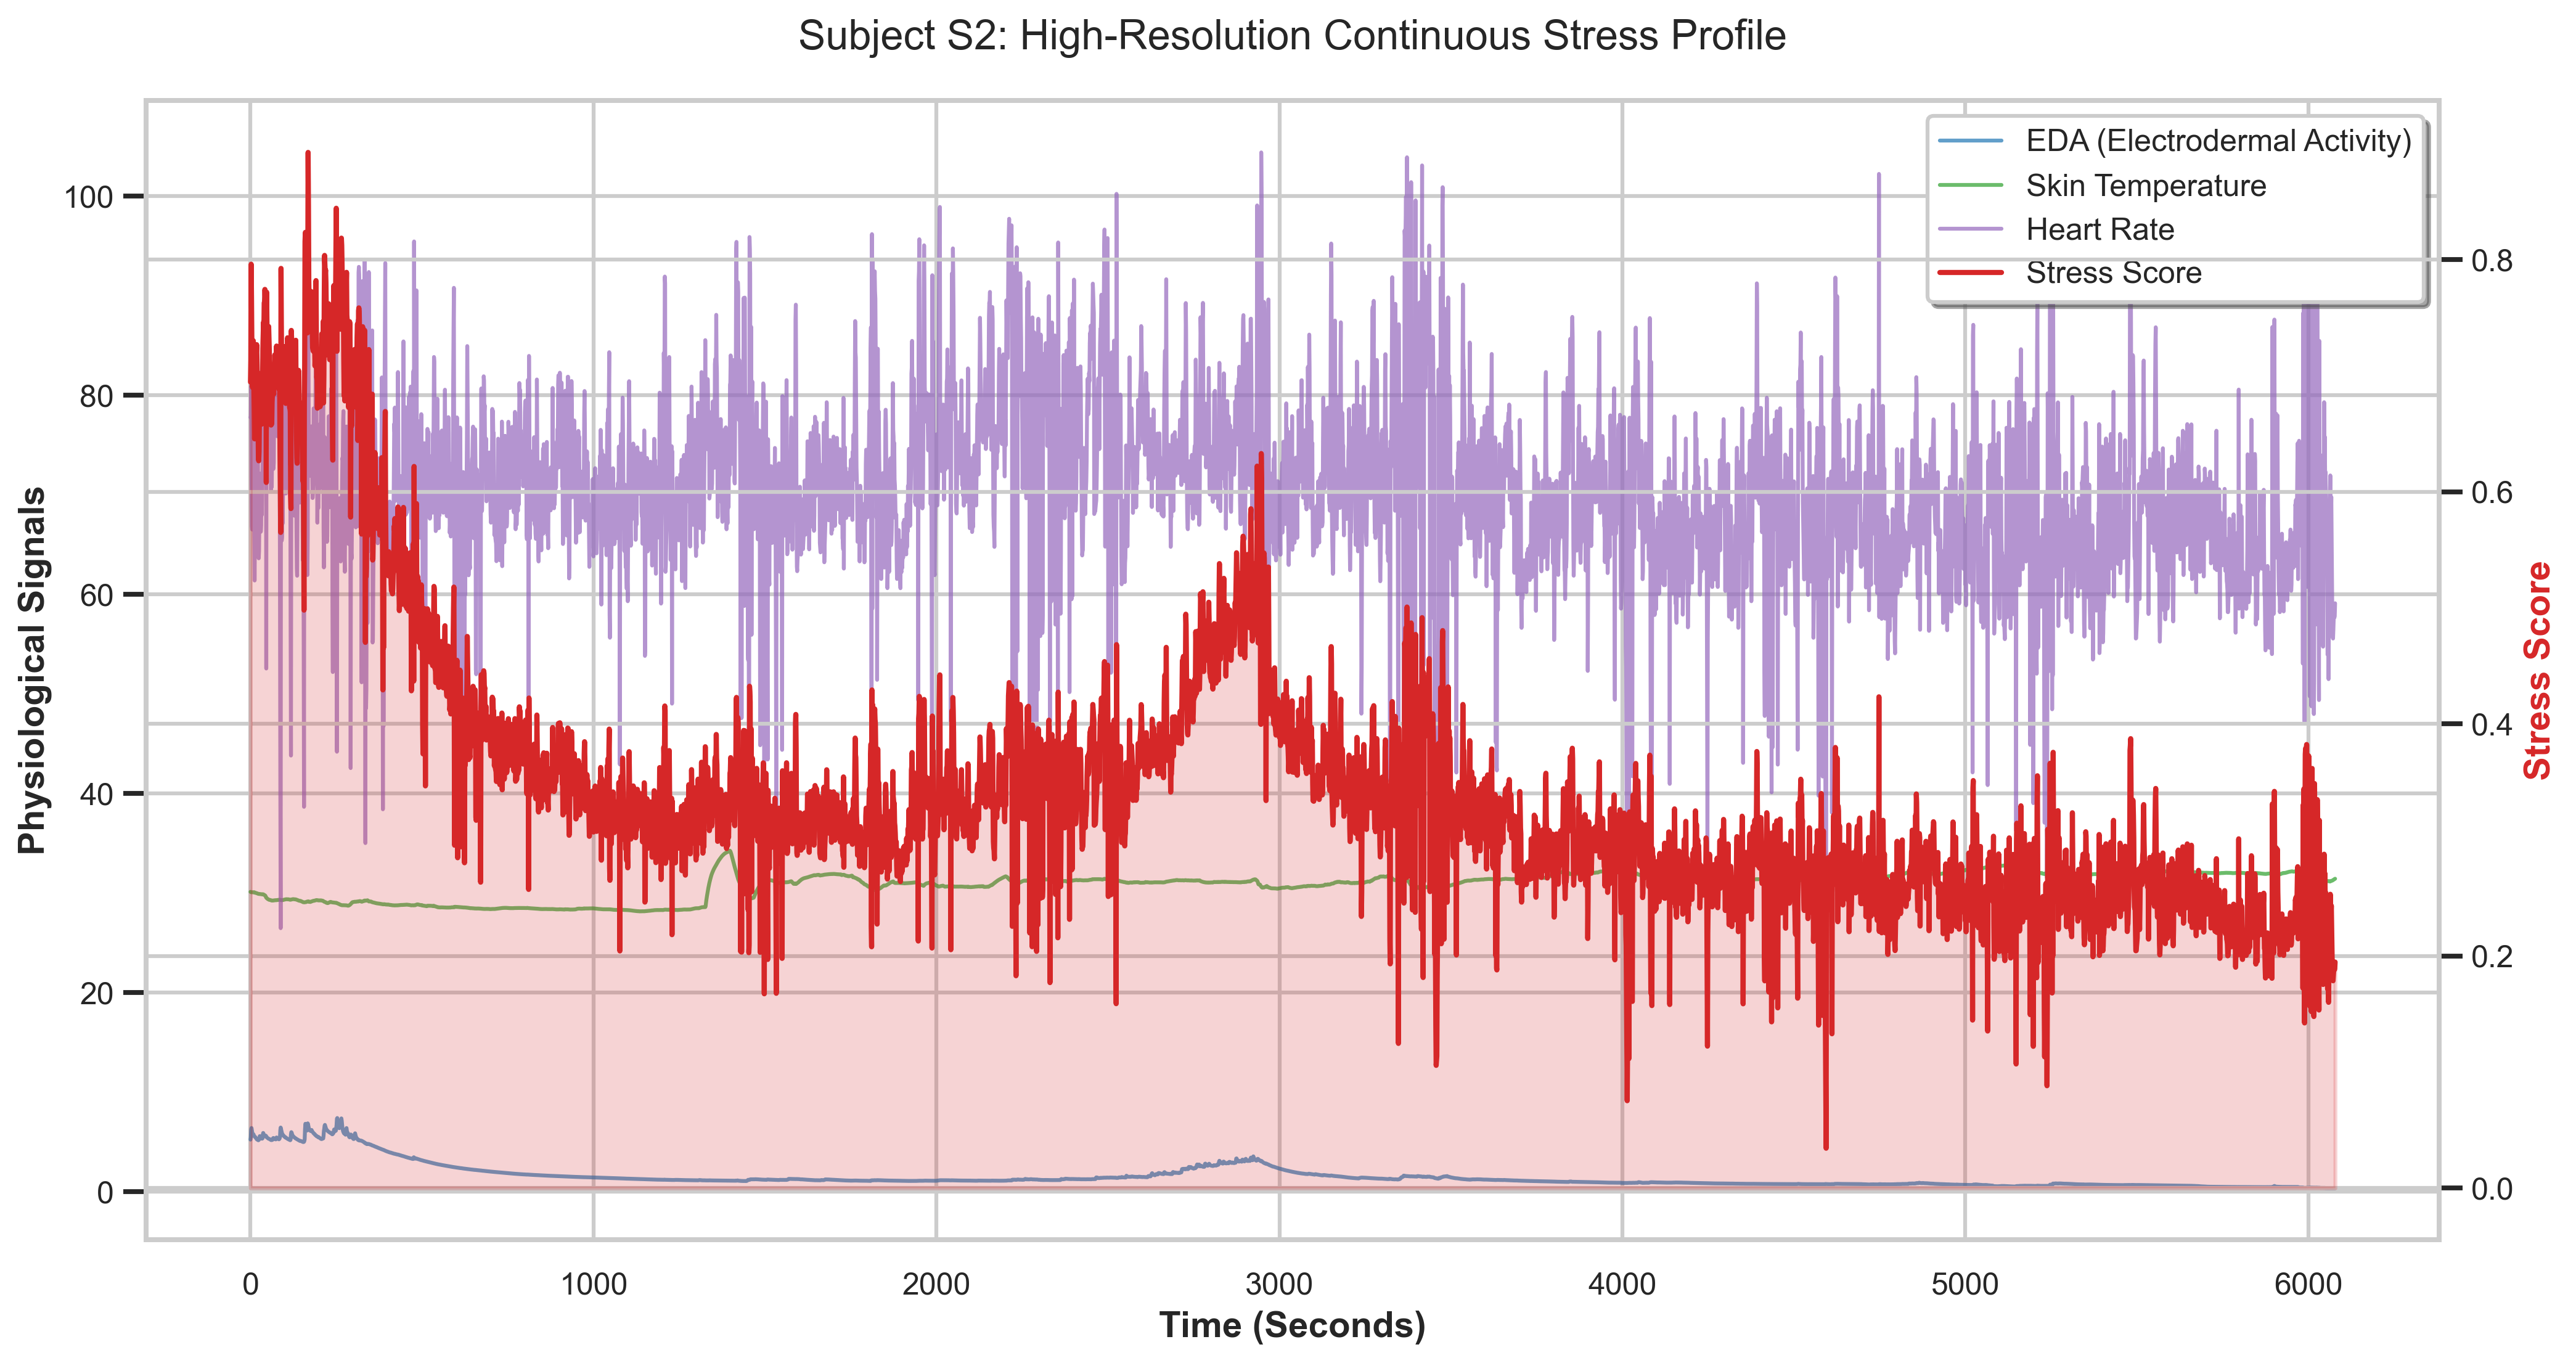
\includegraphics[width=0.9\textwidth, height=0.7\textheight, keepaspectratio]{EDA_Graphs/01_S2_Proper_Timeline.png}
\end{frame}
\begin{frame}{Visualizing Subject S3 (Cross-Audit)}
    \centering 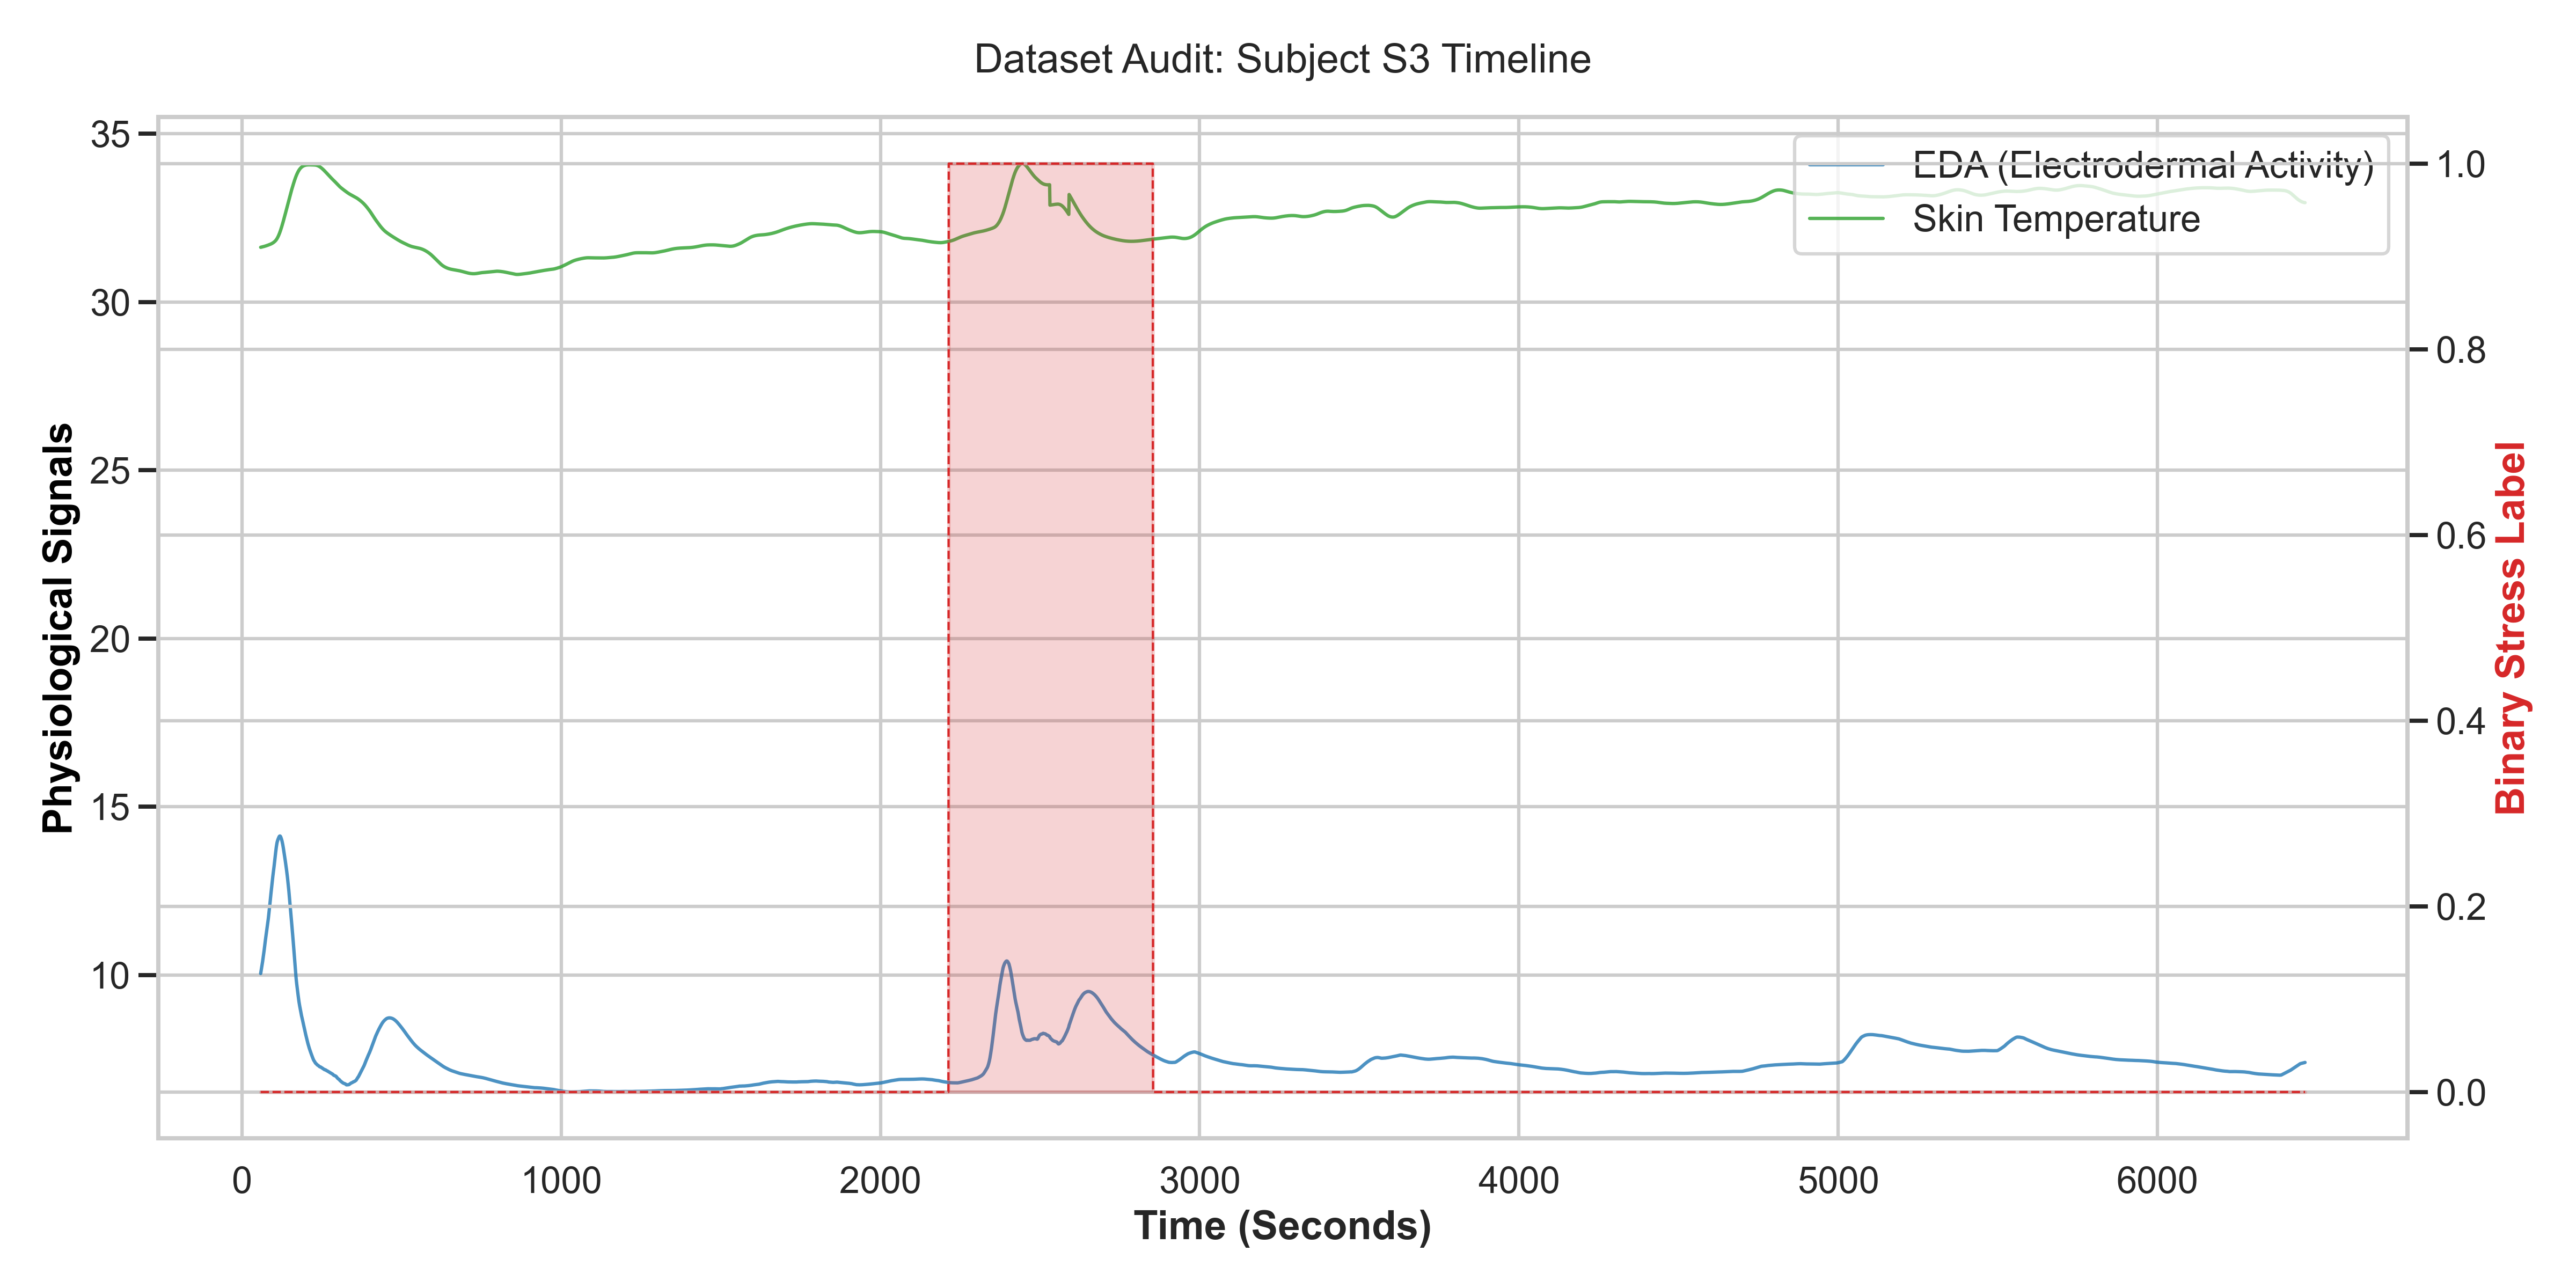
\includegraphics[width=0.9\textwidth, height=0.7\textheight, keepaspectratio]{EDA_Graphs/01_Subject_S3_Timeline.png}
\end{frame}
\begin{frame}{Feature Correlation Heatmap}
    \centering 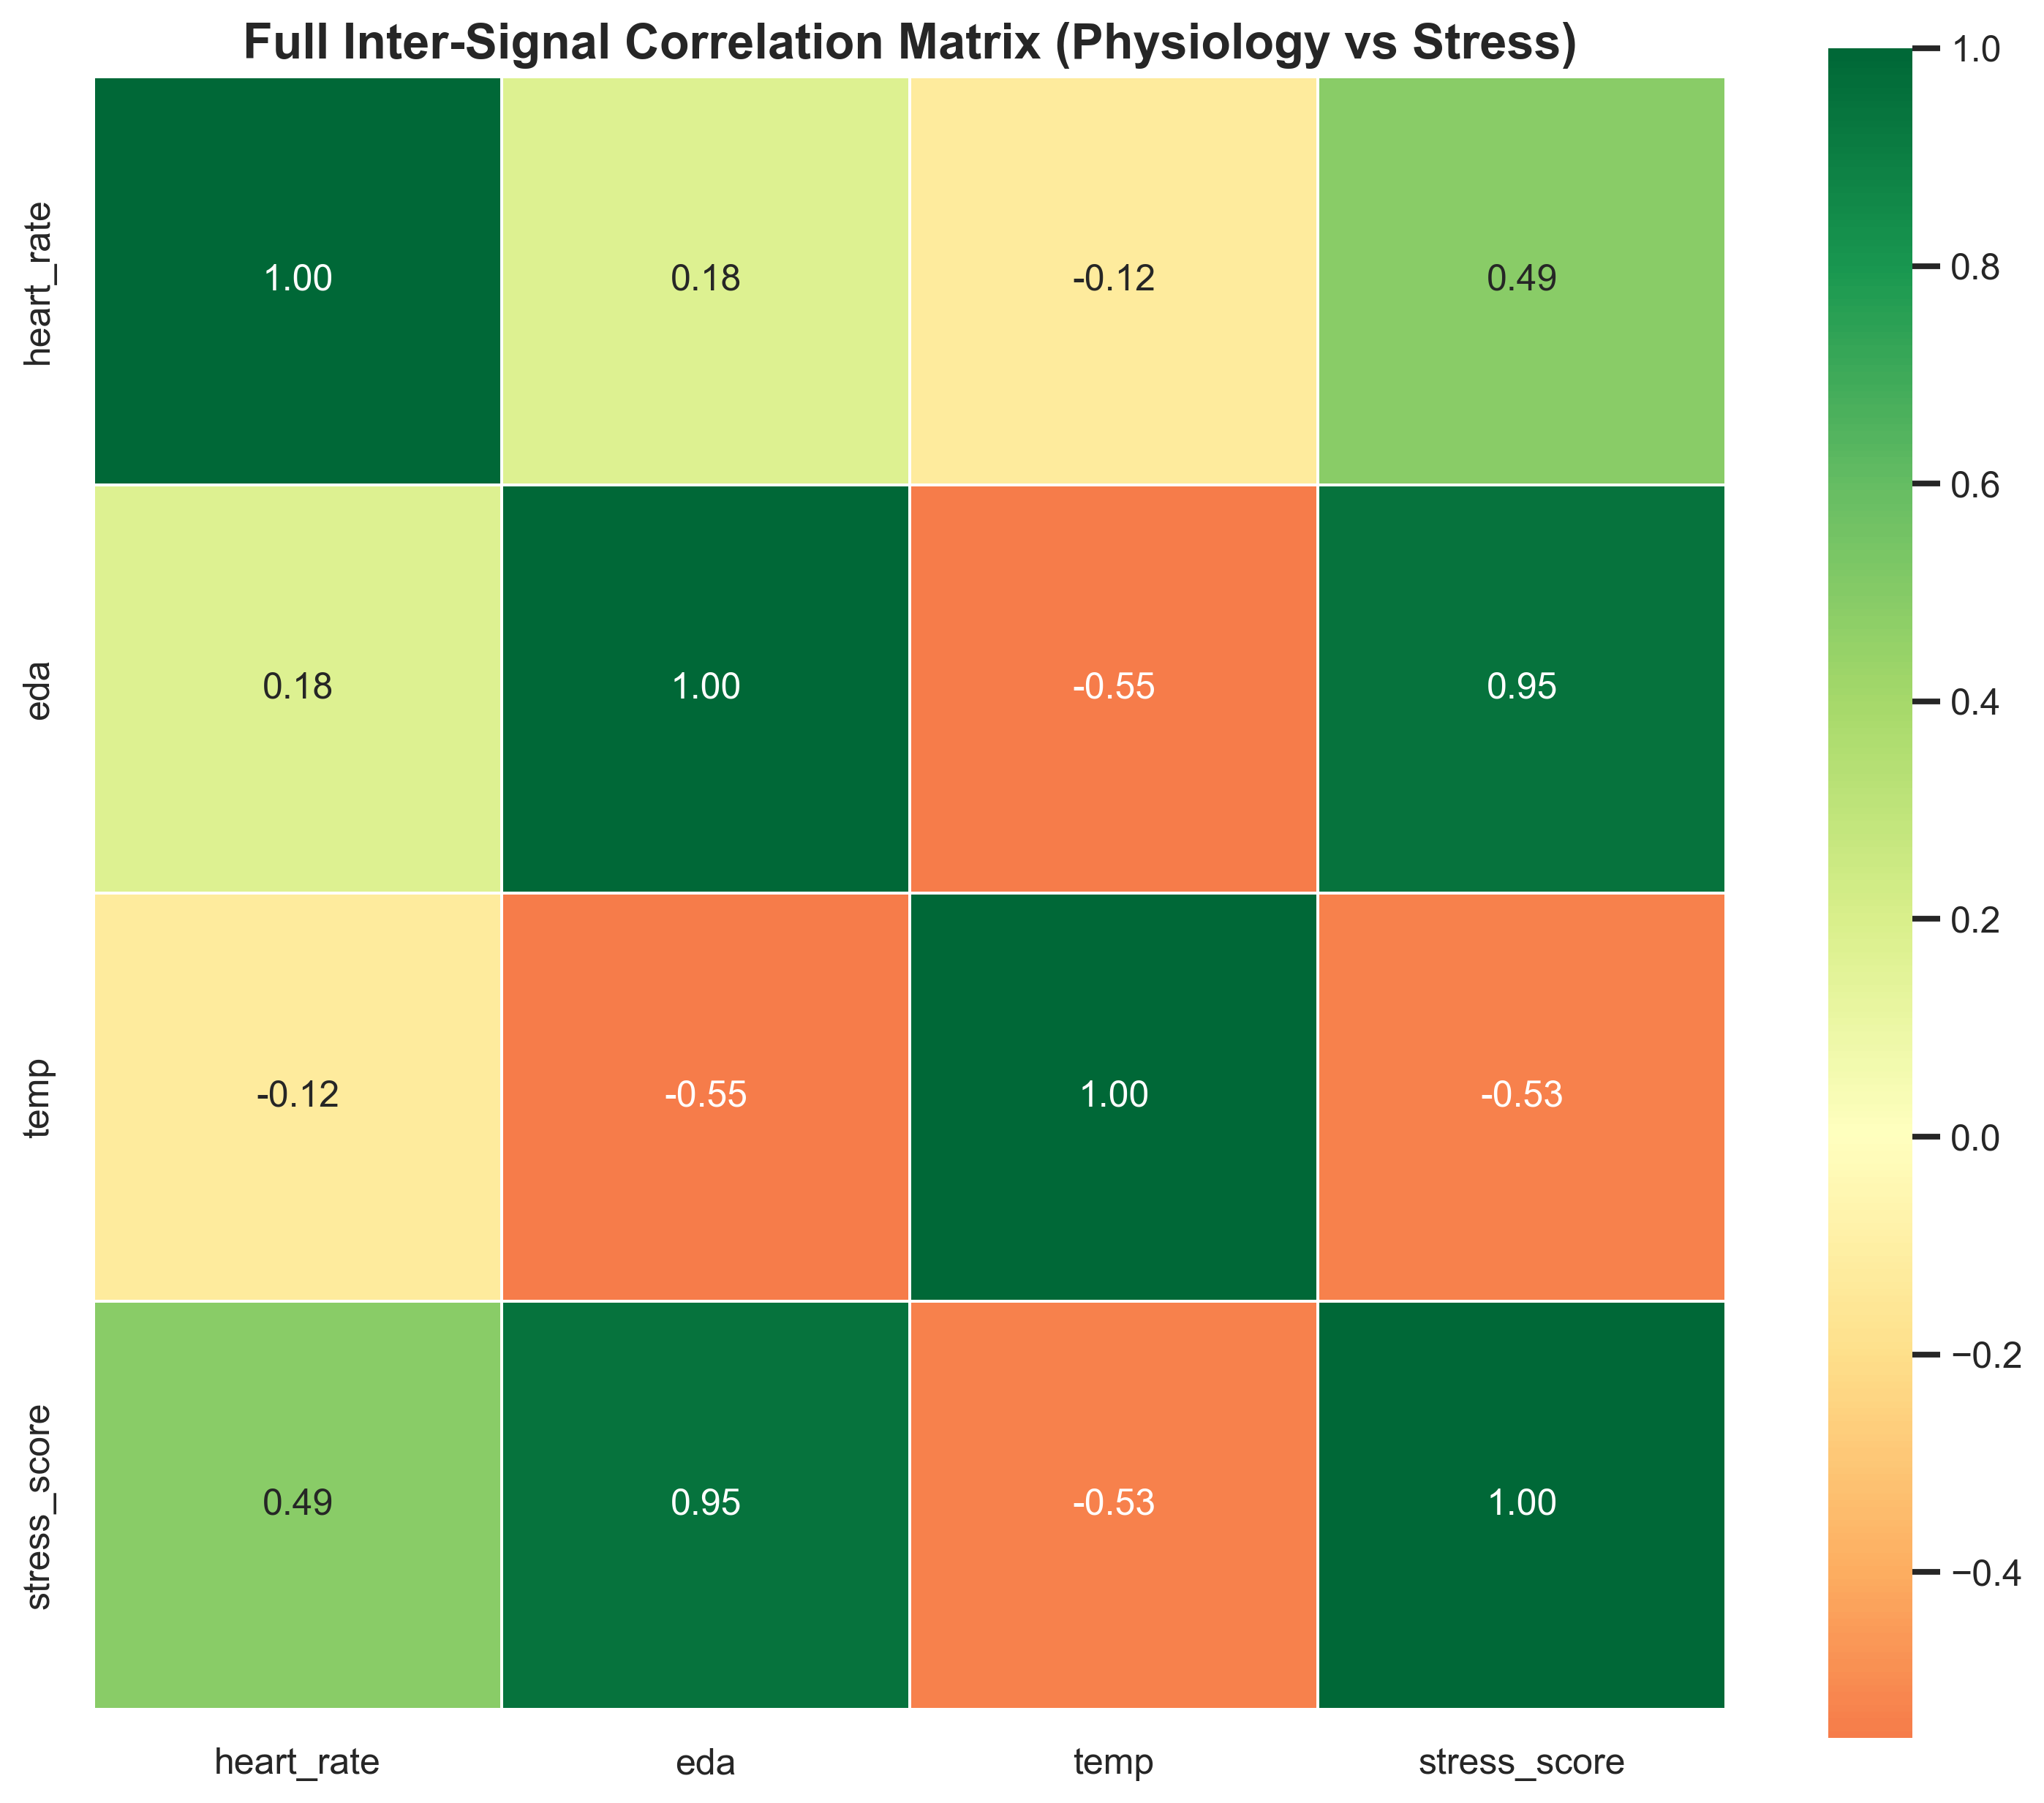
\includegraphics[width=0.75\textwidth, height=0.7\textheight, keepaspectratio]{EDA_Graphs/03_S2_Proper_Correlation.png}
\end{frame}
\begin{frame}{Feature Density (KDE) Analysis}
    \centering 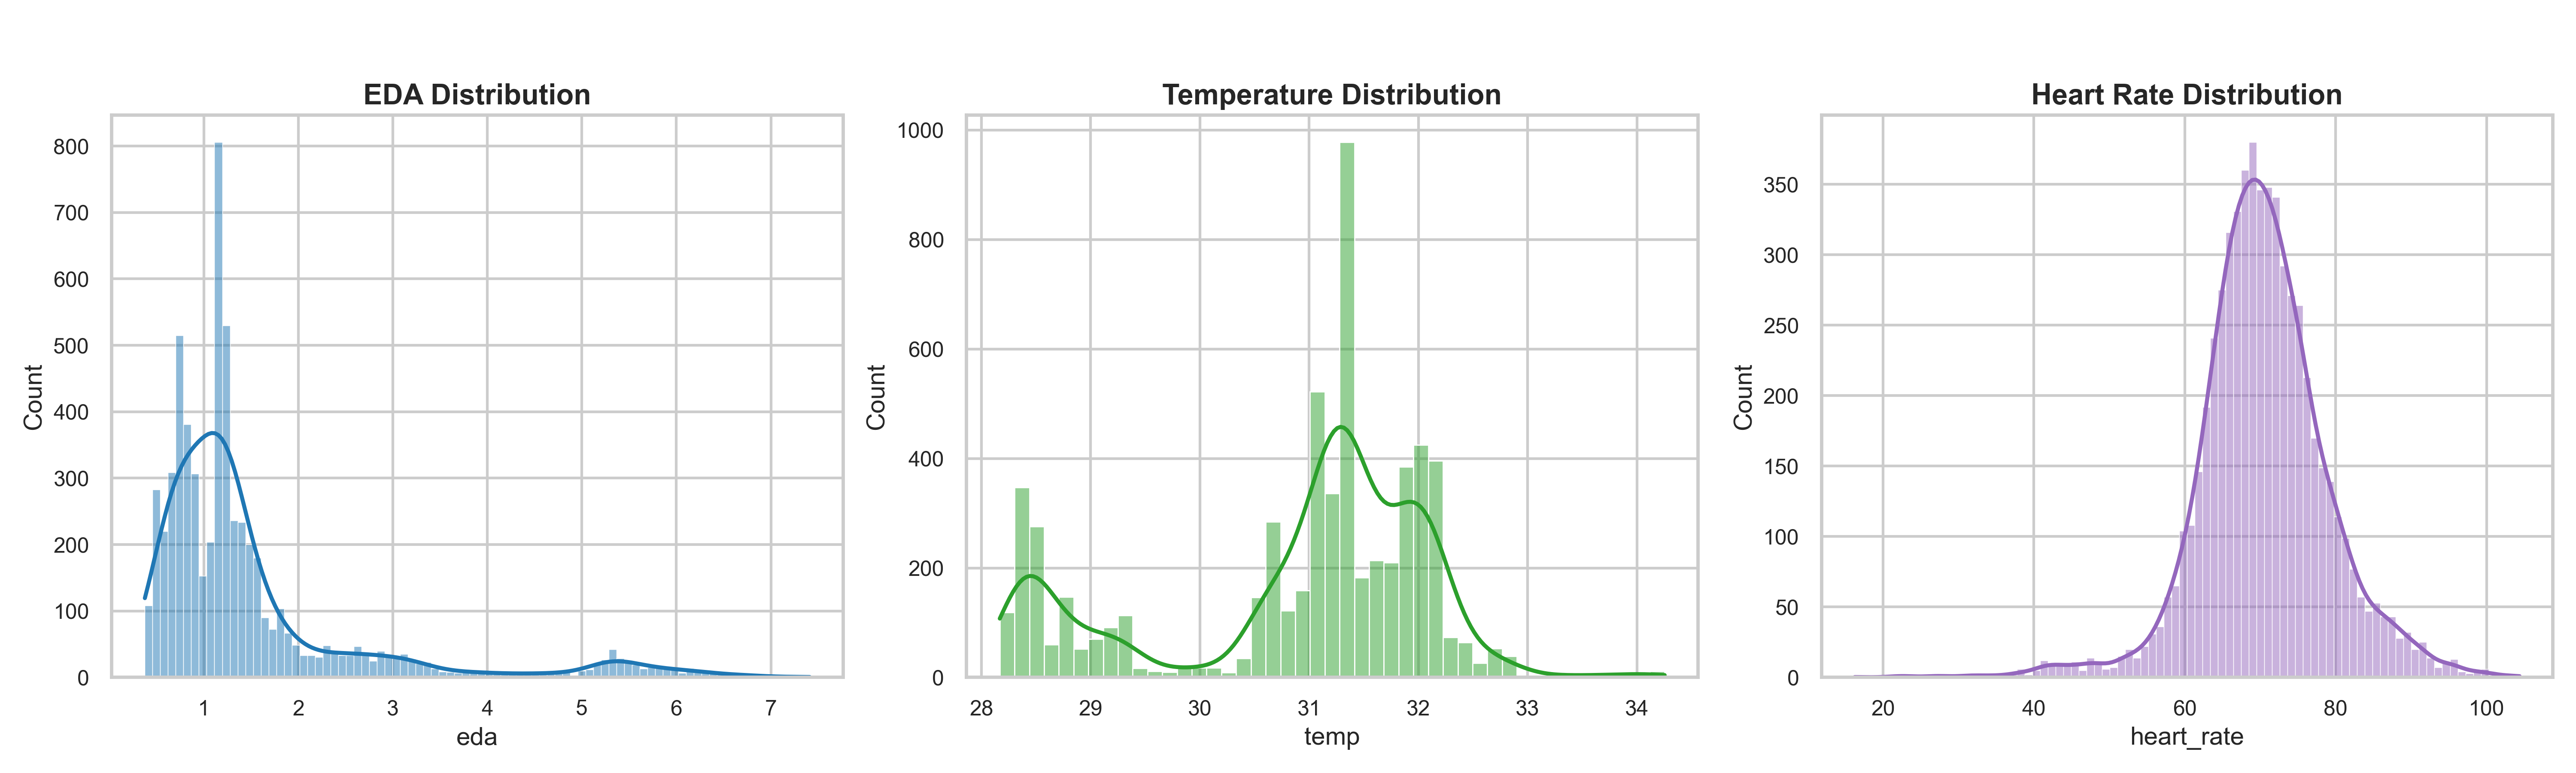
\includegraphics[width=0.9\textwidth, height=0.7\textheight, keepaspectratio]{EDA_Graphs/02_Feature_Density_Analysis.png}
\end{frame}

% ==========================================
% PART 3: ENGINEERING
% ==========================================
\newchapter{III}{Pipeline Engineering \& Error Fixing}
\begin{frame}{Engineering Fix 1: Resolving the Binary Box}
    \textbf{\textcolor{VibrantAmber}{Target Transformation}}
    \vspace{0.4cm}
    \begin{itemize}
        \item \textbf{Mistake:} Using raw 0/1 labels created "staircase" signals.
        \item \textbf{Fix:} Smoothed discrete labels into a 0.0-1.0 \textbf{Stress Intensity Score}.
        \item \textbf{Impact:} Models can now learn the slope of stress onset.
    \end{itemize}
\end{frame}

\begin{frame}{Engineering Fix 2: Anti-Leakage Lag Strategy}
    \textbf{\textcolor{VibrantAmber}{Guaranteeing Validity}}
    \vspace{0.4cm}
    \begin{itemize}
        \item \textbf{Mistake:} Using HR(t) to predict Stress(t) is "cheating" (concurrent detection).
        \item \textbf{Fix:} Every sensor predictor was shifted back by 1 second.
        \item \textbf{Result:} A pure forecast engine: History $\rightarrow$ Future.
    \end{itemize}
\end{frame}

\begin{frame}{Engineering Fix 3: Differencing for Stationarity}
    \textbf{\textcolor{VibrantAmber}{Satisfying Mathematical Priors}}
    \vspace{0.4cm}
    \begin{itemize}
        \item \textbf{Discovery:} ADF test proved stress signal had a "drift" ($p > 0.05$).
        \item \textbf{Fix:} Applied First-Order Differencing ($d=1$).
        \item \textbf{Result:} Stationary signal oscillating around zero mean.
    \end{itemize}
\end{frame}

\begin{frame}{Differencing Visualization}
    \centering 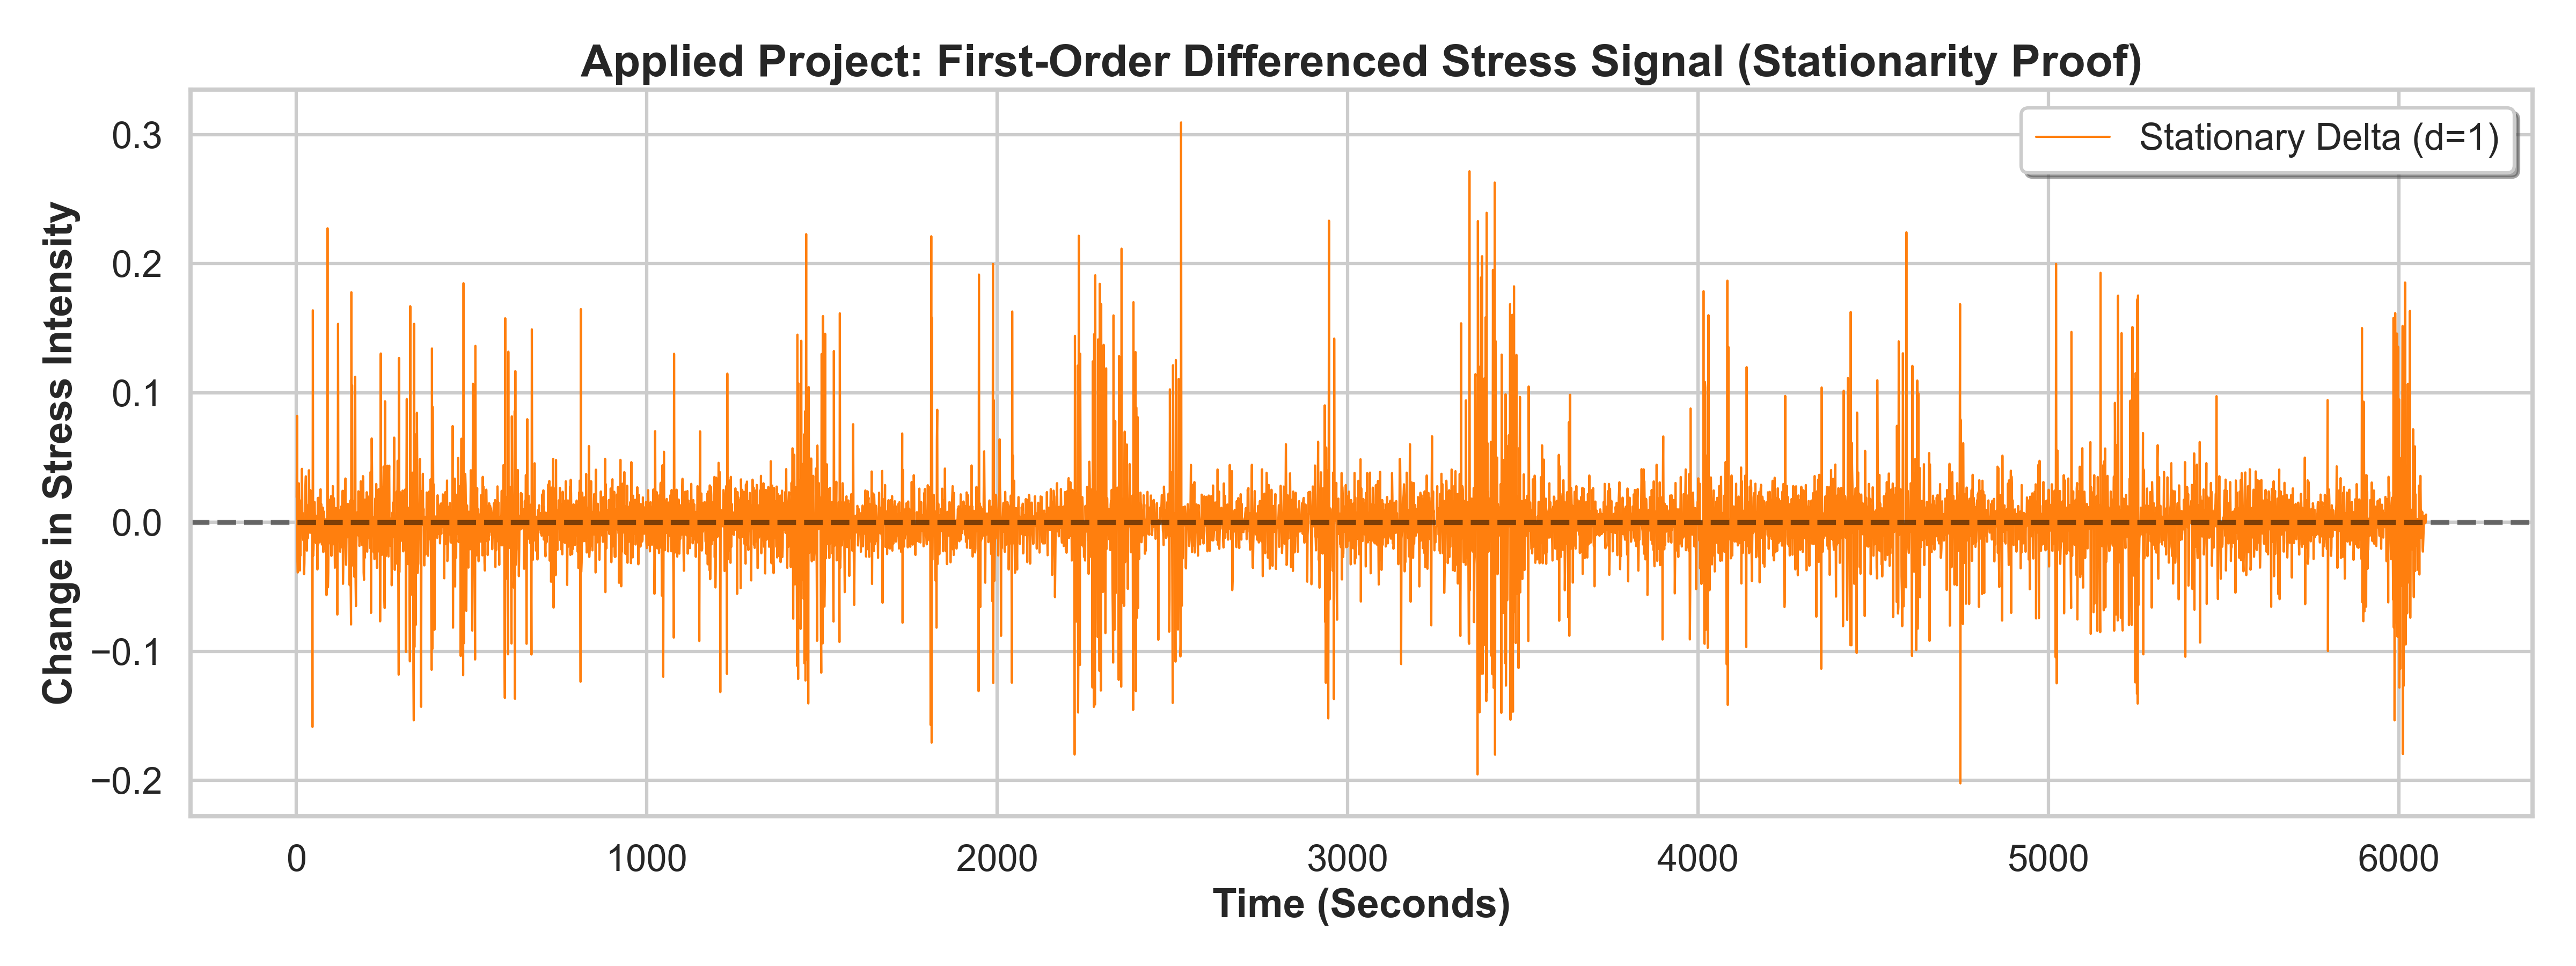
\includegraphics[width=0.9\textwidth, height=0.7\textheight, keepaspectratio]{EDA_Graphs/05_Differenced_Signal_Timeline.png}
\end{frame}

% ==========================================
% PART 4: MODELS
% ==========================================
\newchapter{IV}{The 13 Models Deep-Dive}

% 1. Naive
\begin{frame}{Model 1 Theory: Naive Persistence}
    \textbf{\textcolor{VibrantAmber}{Theoretical Foundation}}
    \vspace{0.2cm}
    The simplest baseline for 1Hz series. Assumes the current state persists.
    \vspace{0.3cm}
    \begin{tcolorbox}[colback=Midnight!5, colframe=Midnight, title=\textbf{Equation}]
        \[ \hat{y}_{t+1} = y_t \]
    \end{tcolorbox}
\end{frame}
\begin{frame}{Model 1 Result: Naive Persistence}
    \begin{columns}
        \begin{column}{0.65\textwidth} 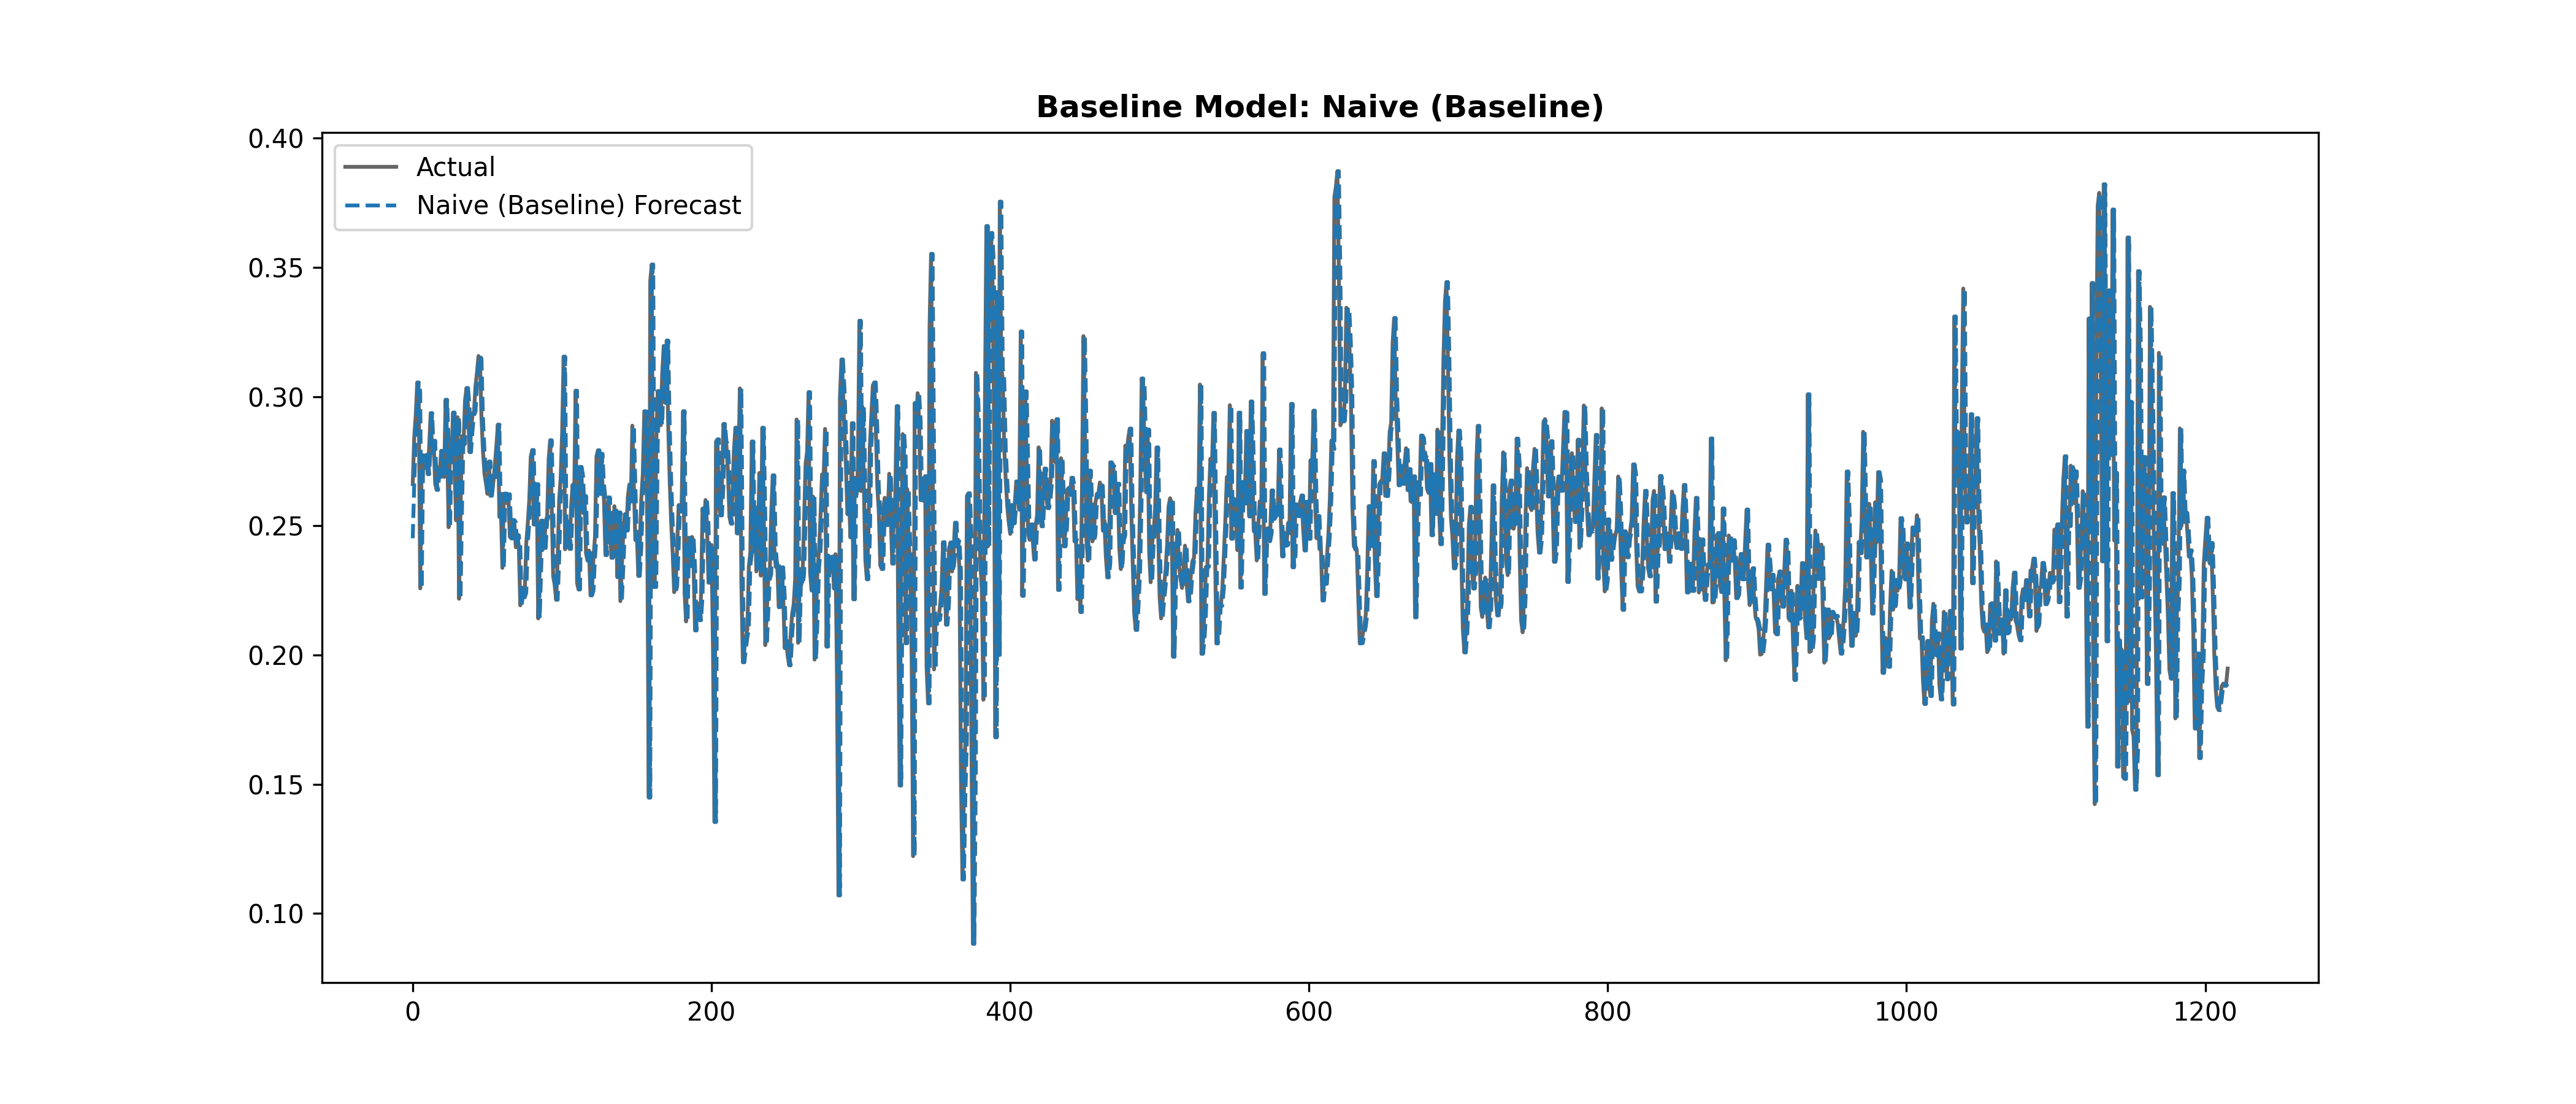
\includegraphics[width=\textwidth, height=0.7\textheight, keepaspectratio]{Forecasting_Graphs/00_Naive_(Baseline).png} \end{column}
        \begin{column}{0.33\textwidth} \metricwidget{Naive}{0.0211}{0.0345}{8.68}{0.0673} \end{column}
    \end{columns}
\end{frame}

% 2. SMA
\begin{frame}{Model 2 Theory: SMA-10}
    \textbf{\textcolor{VibrantAmber}{Theoretical Foundation}}
    Simple Moving Average over 10 seconds. Filters out micro-jitter.
    \vspace{0.3cm}
    \begin{tcolorbox}[colback=Midnight!5, colframe=Midnight, title=\textbf{Equation}]
        \[ \hat{y}_{t+1} = \frac{1}{k} \sum_{i=0}^{k-1} y_{t-i} \]
    \end{tcolorbox}
\end{frame}
\begin{frame}{Model 2 Result: SMA-10}
    \begin{columns}
        \begin{column}{0.65\textwidth} 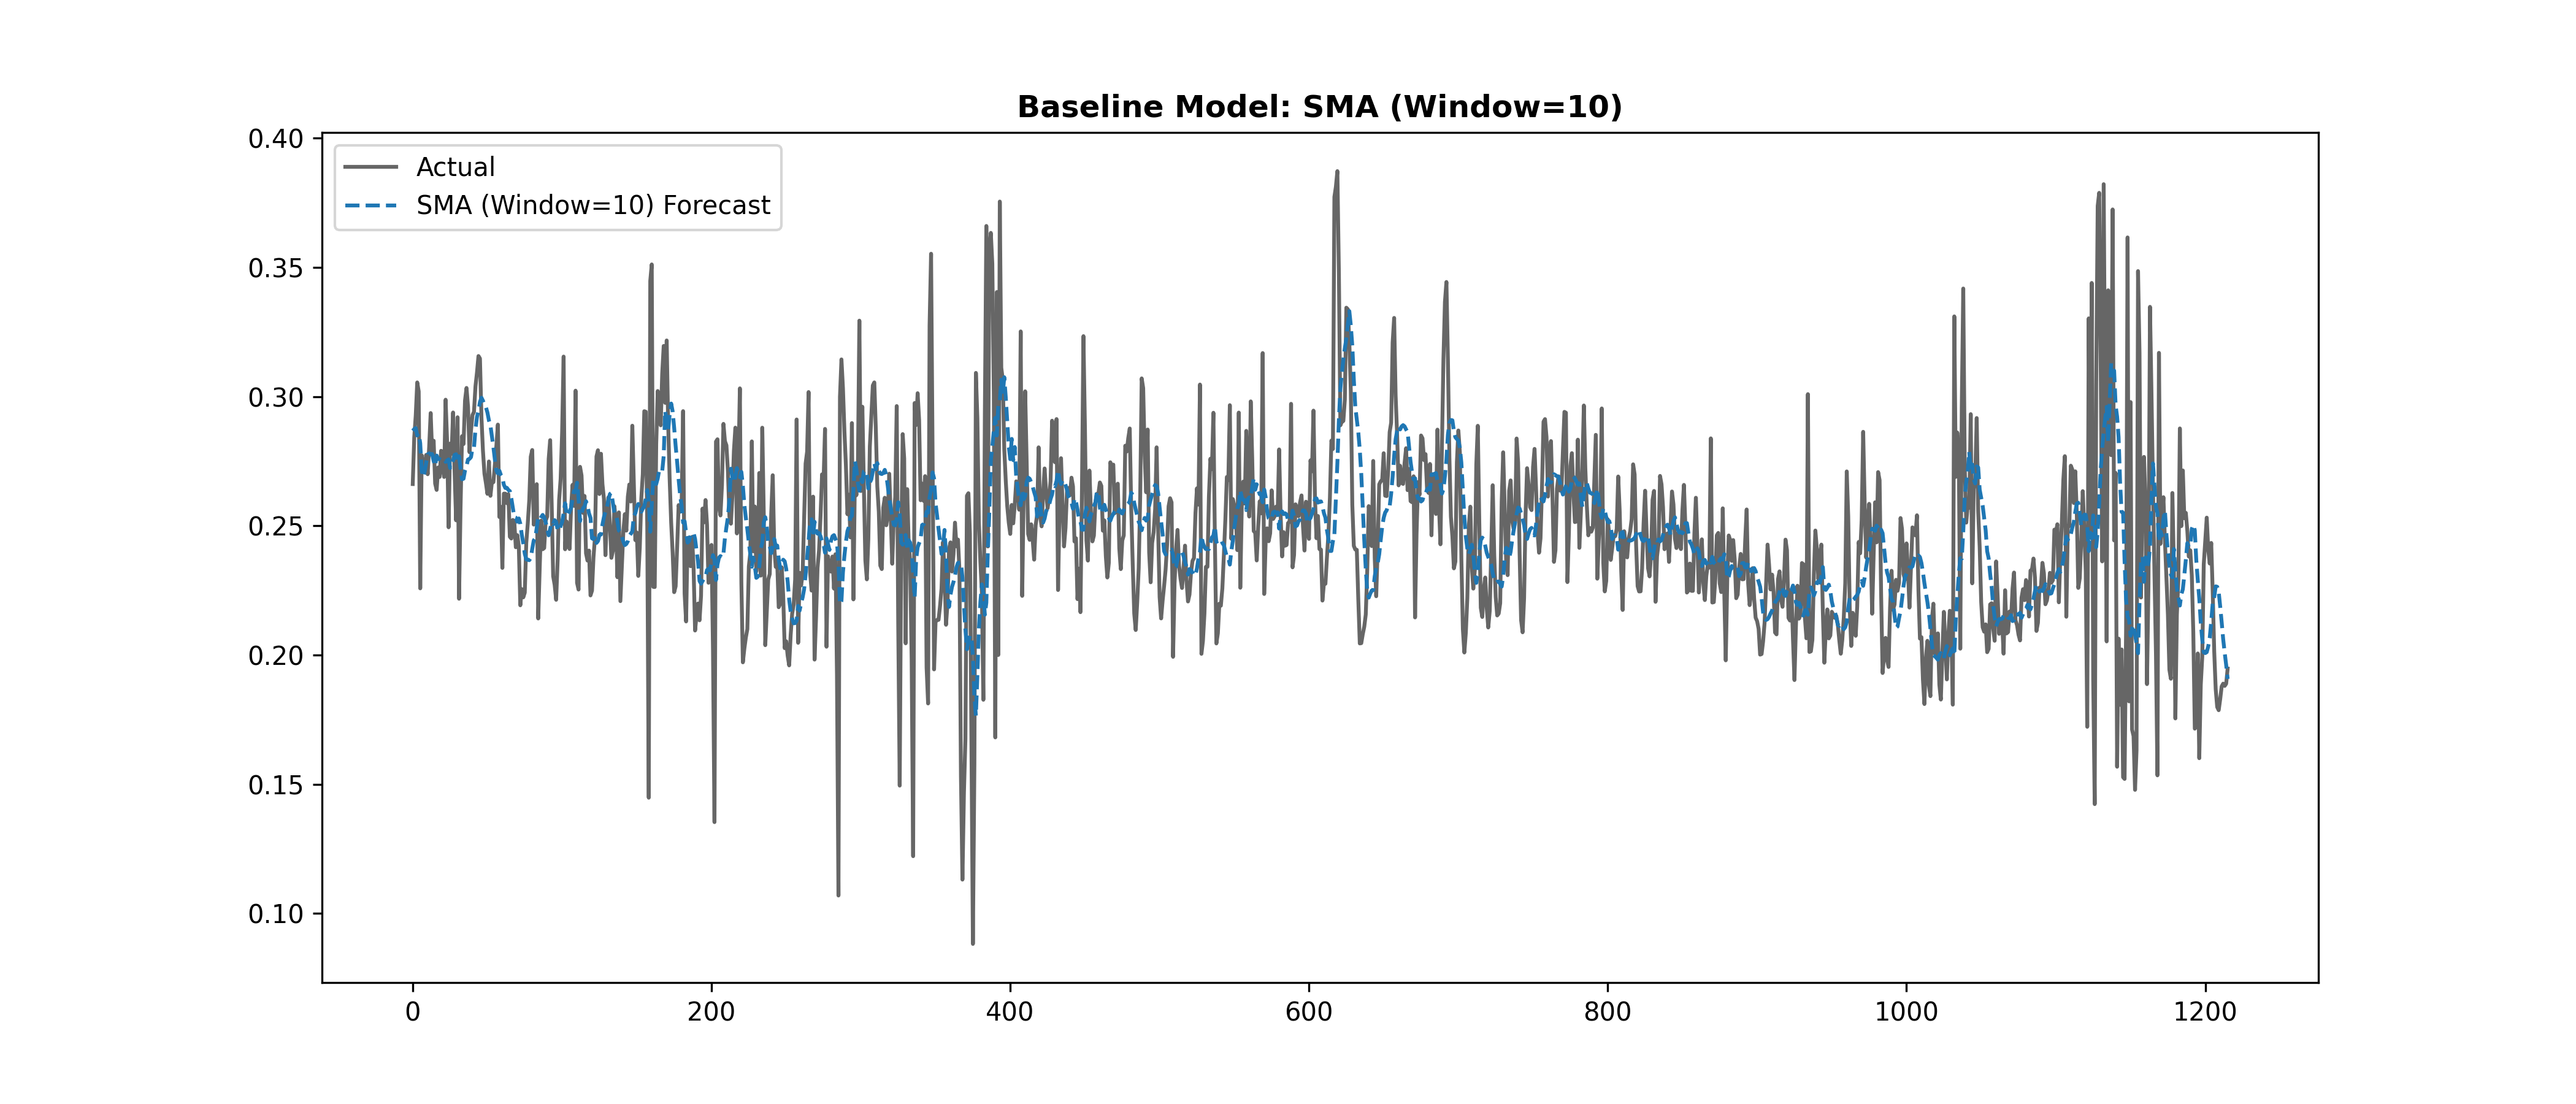
\includegraphics[width=\textwidth, height=0.7\textheight, keepaspectratio]{Forecasting_Graphs/00_SMA_(Window=10).png} \end{column}
        \begin{column}{0.33\textwidth} \metricwidget{SMA-10}{0.0229}{0.0326}{9.62}{0.1716} \end{column}
    \end{columns}
\end{frame}

% 3. AR
\begin{frame}{Model 3 Theory: AR(2)}
    \textbf{\textcolor{VibrantAmber}{Theoretical Foundation}}
    AutoRegressive model using lag-2 memory based on PACF audit.
    \vspace{0.3cm}
    \begin{tcolorbox}[colback=Midnight!5, colframe=Midnight, title=\textbf{Equation}]
        \[ y_t = c + \phi_1 y_{t-1} + \phi_2 y_{t-2} + \epsilon_t \]
    \end{tcolorbox}
\end{frame}
\begin{frame}{Model 3 Result: AR(2)}
    \begin{columns}
        \begin{column}{0.65\textwidth} 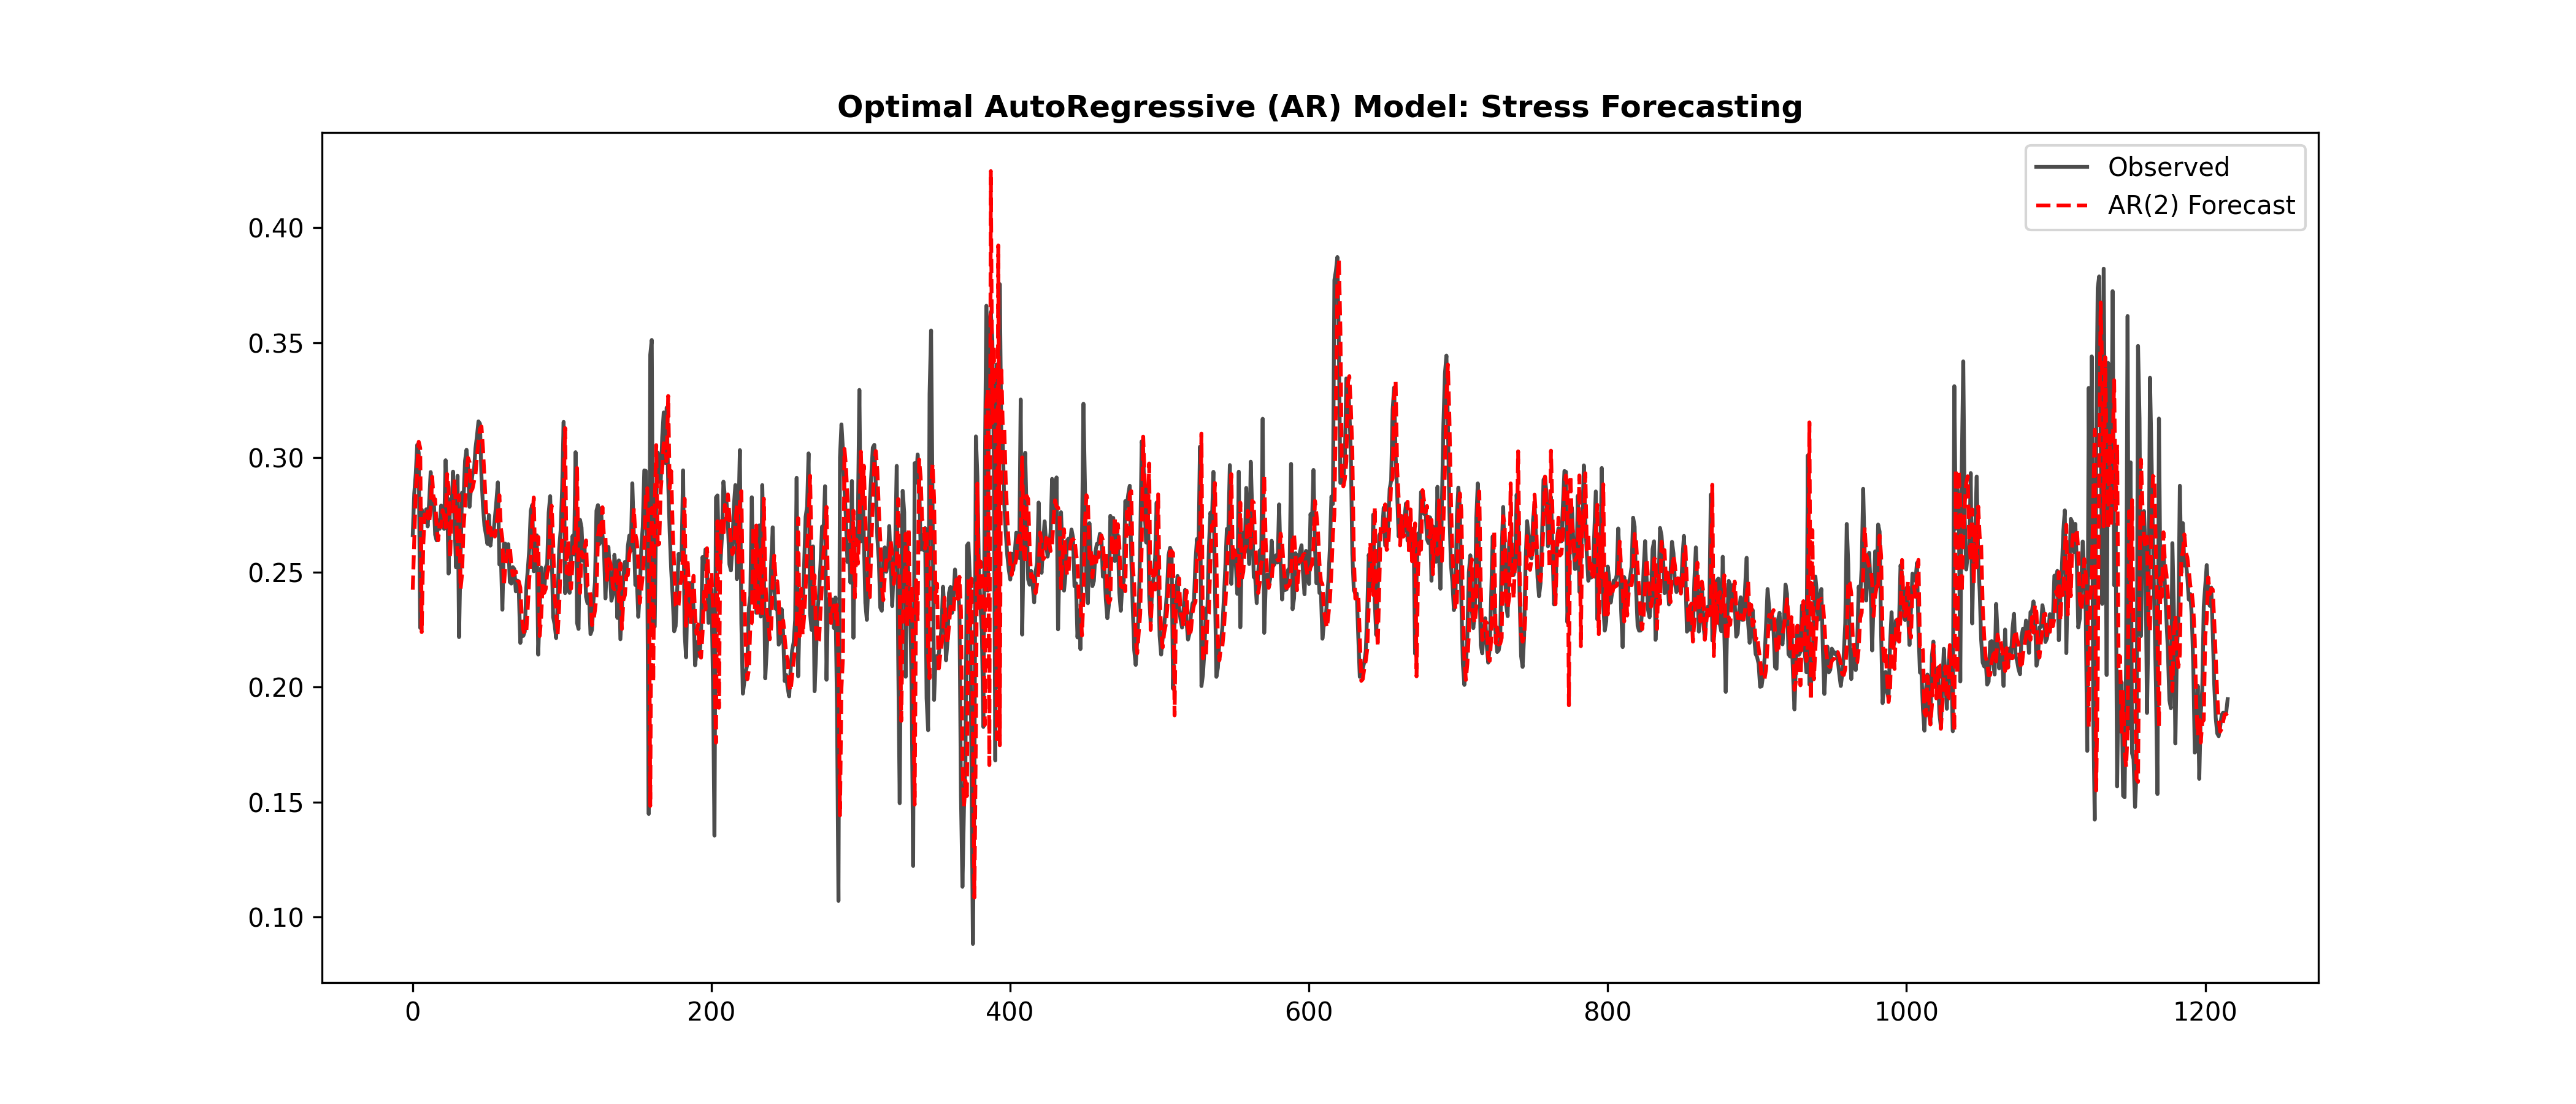
\includegraphics[width=\textwidth, height=0.7\textheight, keepaspectratio]{Forecasting_Graphs/03_AR_Optimized.png} \end{column}
        \begin{column}{0.33\textwidth} \metricwidget{AR(2)}{0.0210}{0.0342}{8.66}{0.0840} \end{column}
    \end{columns}
\end{frame}

% 4. MA
\begin{frame}{Model 4 Theory: MA(3)}
    \textbf{\textcolor{VibrantAmber}{Theoretical Foundation}}
    Moving Average model using 3 error terms based on ACF audit.
    \vspace{0.3cm}
    \begin{tcolorbox}[colback=Midnight!5, colframe=Midnight, title=\textbf{Equation}]
        \[ y_t = \mu + \epsilon_t + \theta_1 \epsilon_{t-1} + \theta_2 \epsilon_{t-2} + \theta_3 \epsilon_{t-3} \]
    \end{tcolorbox}
\end{frame}
\begin{frame}{Model 4 Result: MA(3)}
    \begin{columns}
        \begin{column}{0.65\textwidth} 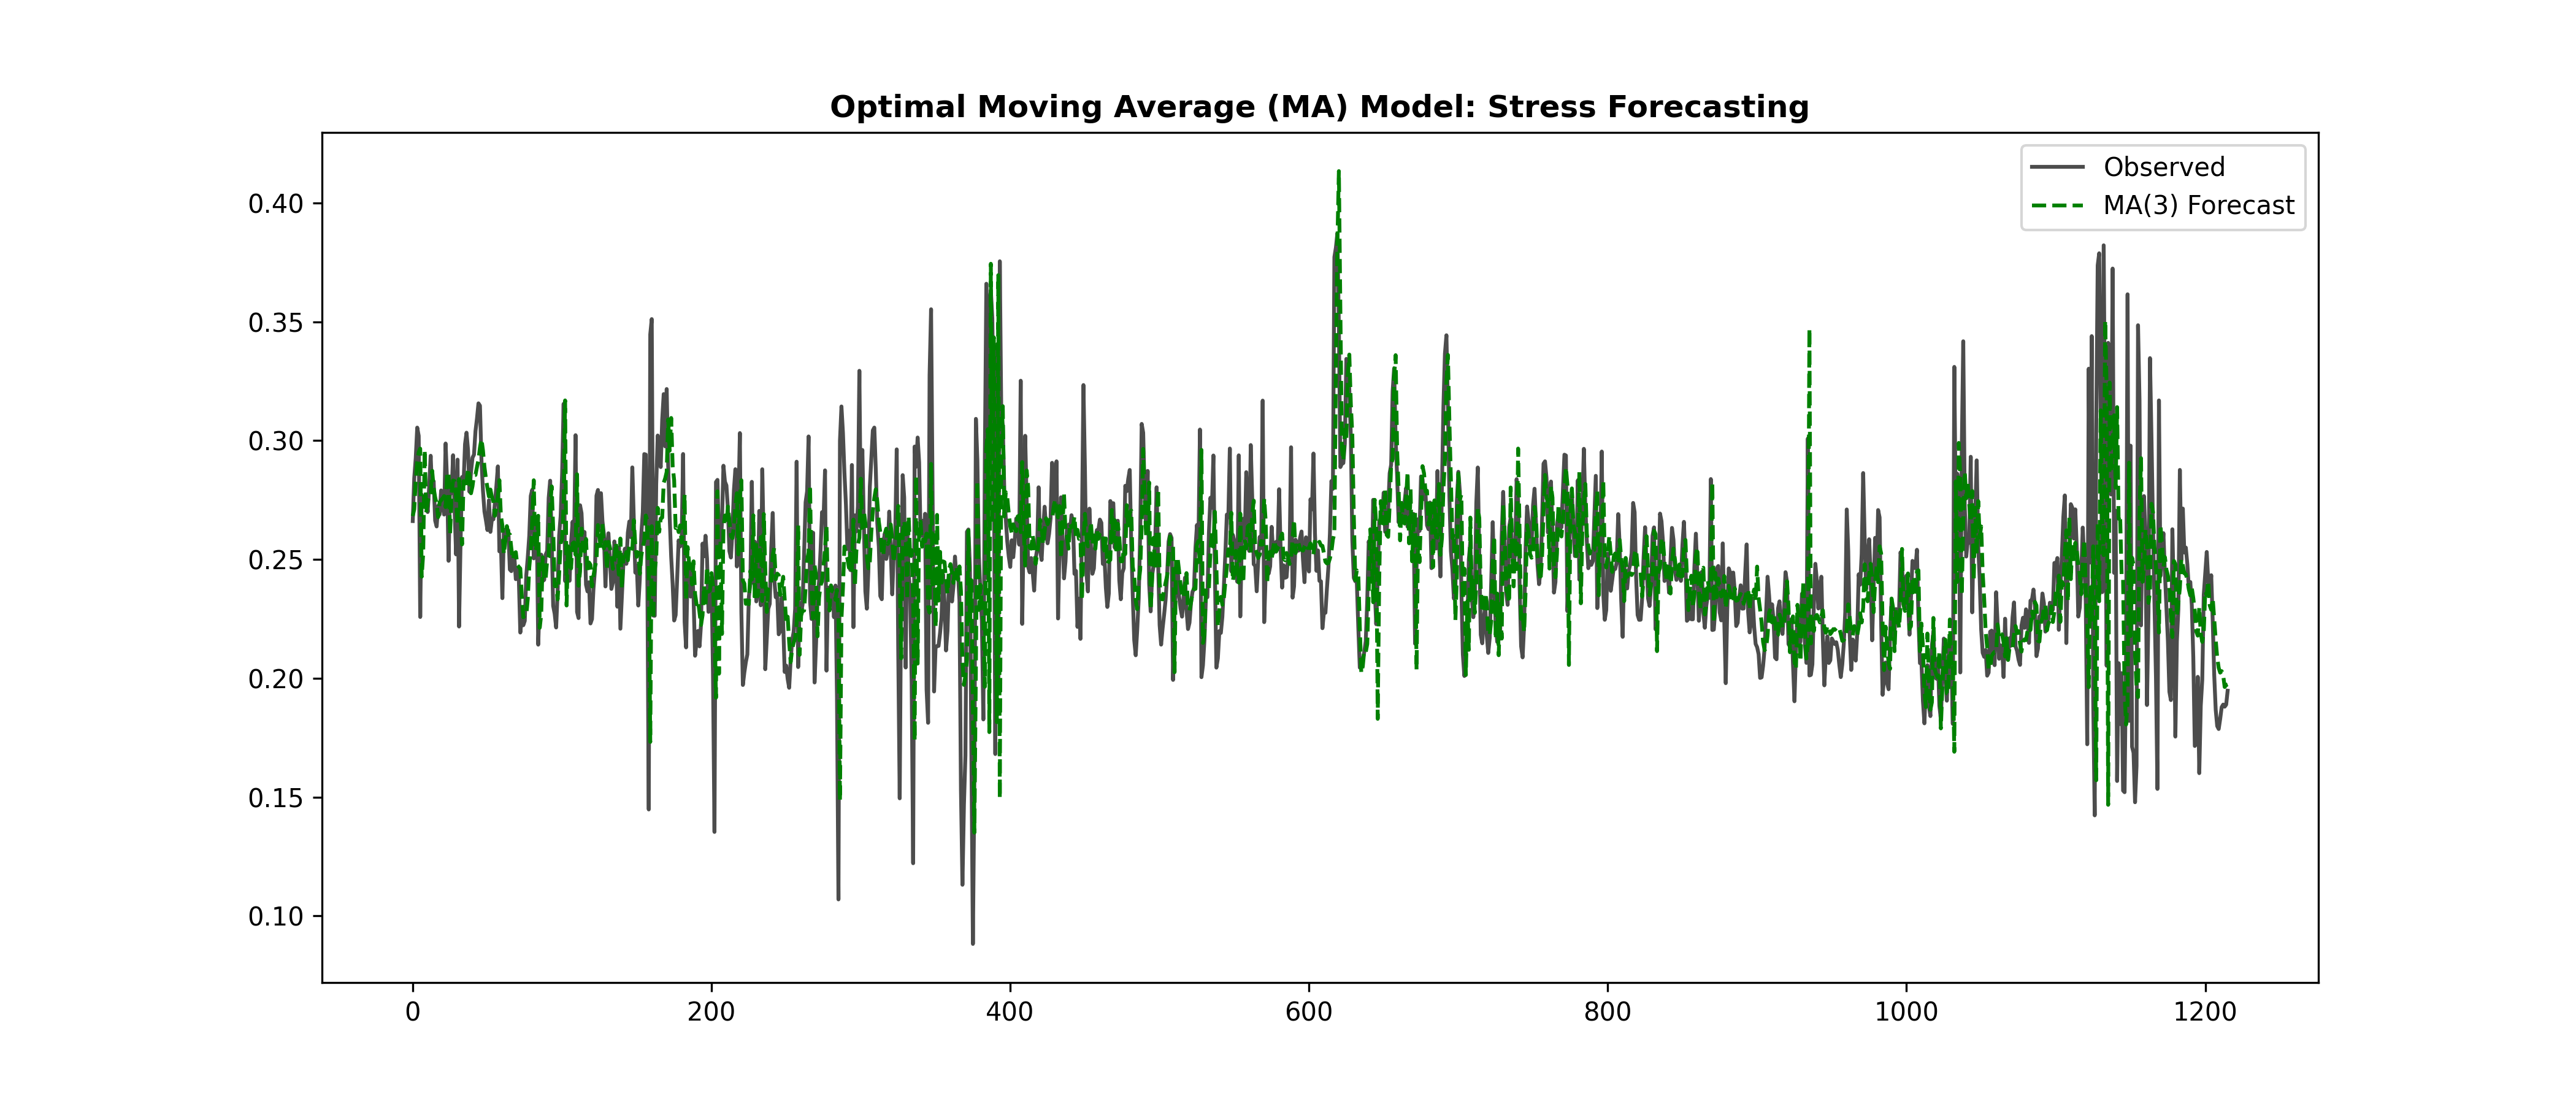
\includegraphics[width=\textwidth, height=0.7\textheight, keepaspectratio]{Forecasting_Graphs/04_MA_Optimized.png} \end{column}
        \begin{column}{0.33\textwidth} \metricwidget{MA(3)}{0.0209}{0.0335}{8.72}{0.1236} \end{column}
    \end{columns}
\end{frame}

% 5. ARMA
\begin{frame}{Model 5 Theory: ARMA(2,3)}
    \textbf{\textcolor{VibrantAmber}{Theoretical Foundation}}
    Optimized hybrid. Represents the linear peak of stress history logic.
    \vspace{0.3cm}
    \begin{tcolorbox}[colback=Midnight!5, colframe=Midnight, title=\textbf{Equation}]
        \[ \hat{y}_t = c + \sum_{i=1}^p \phi_i y_{t-i} + \epsilon_t + \sum_{j=1}^q \theta_j \epsilon_{t-j} \]
    \end{tcolorbox}
\end{frame}
\begin{frame}{Model 5 Result: ARMA(2,3)}
    \begin{columns}
        \begin{column}{0.65\textwidth} 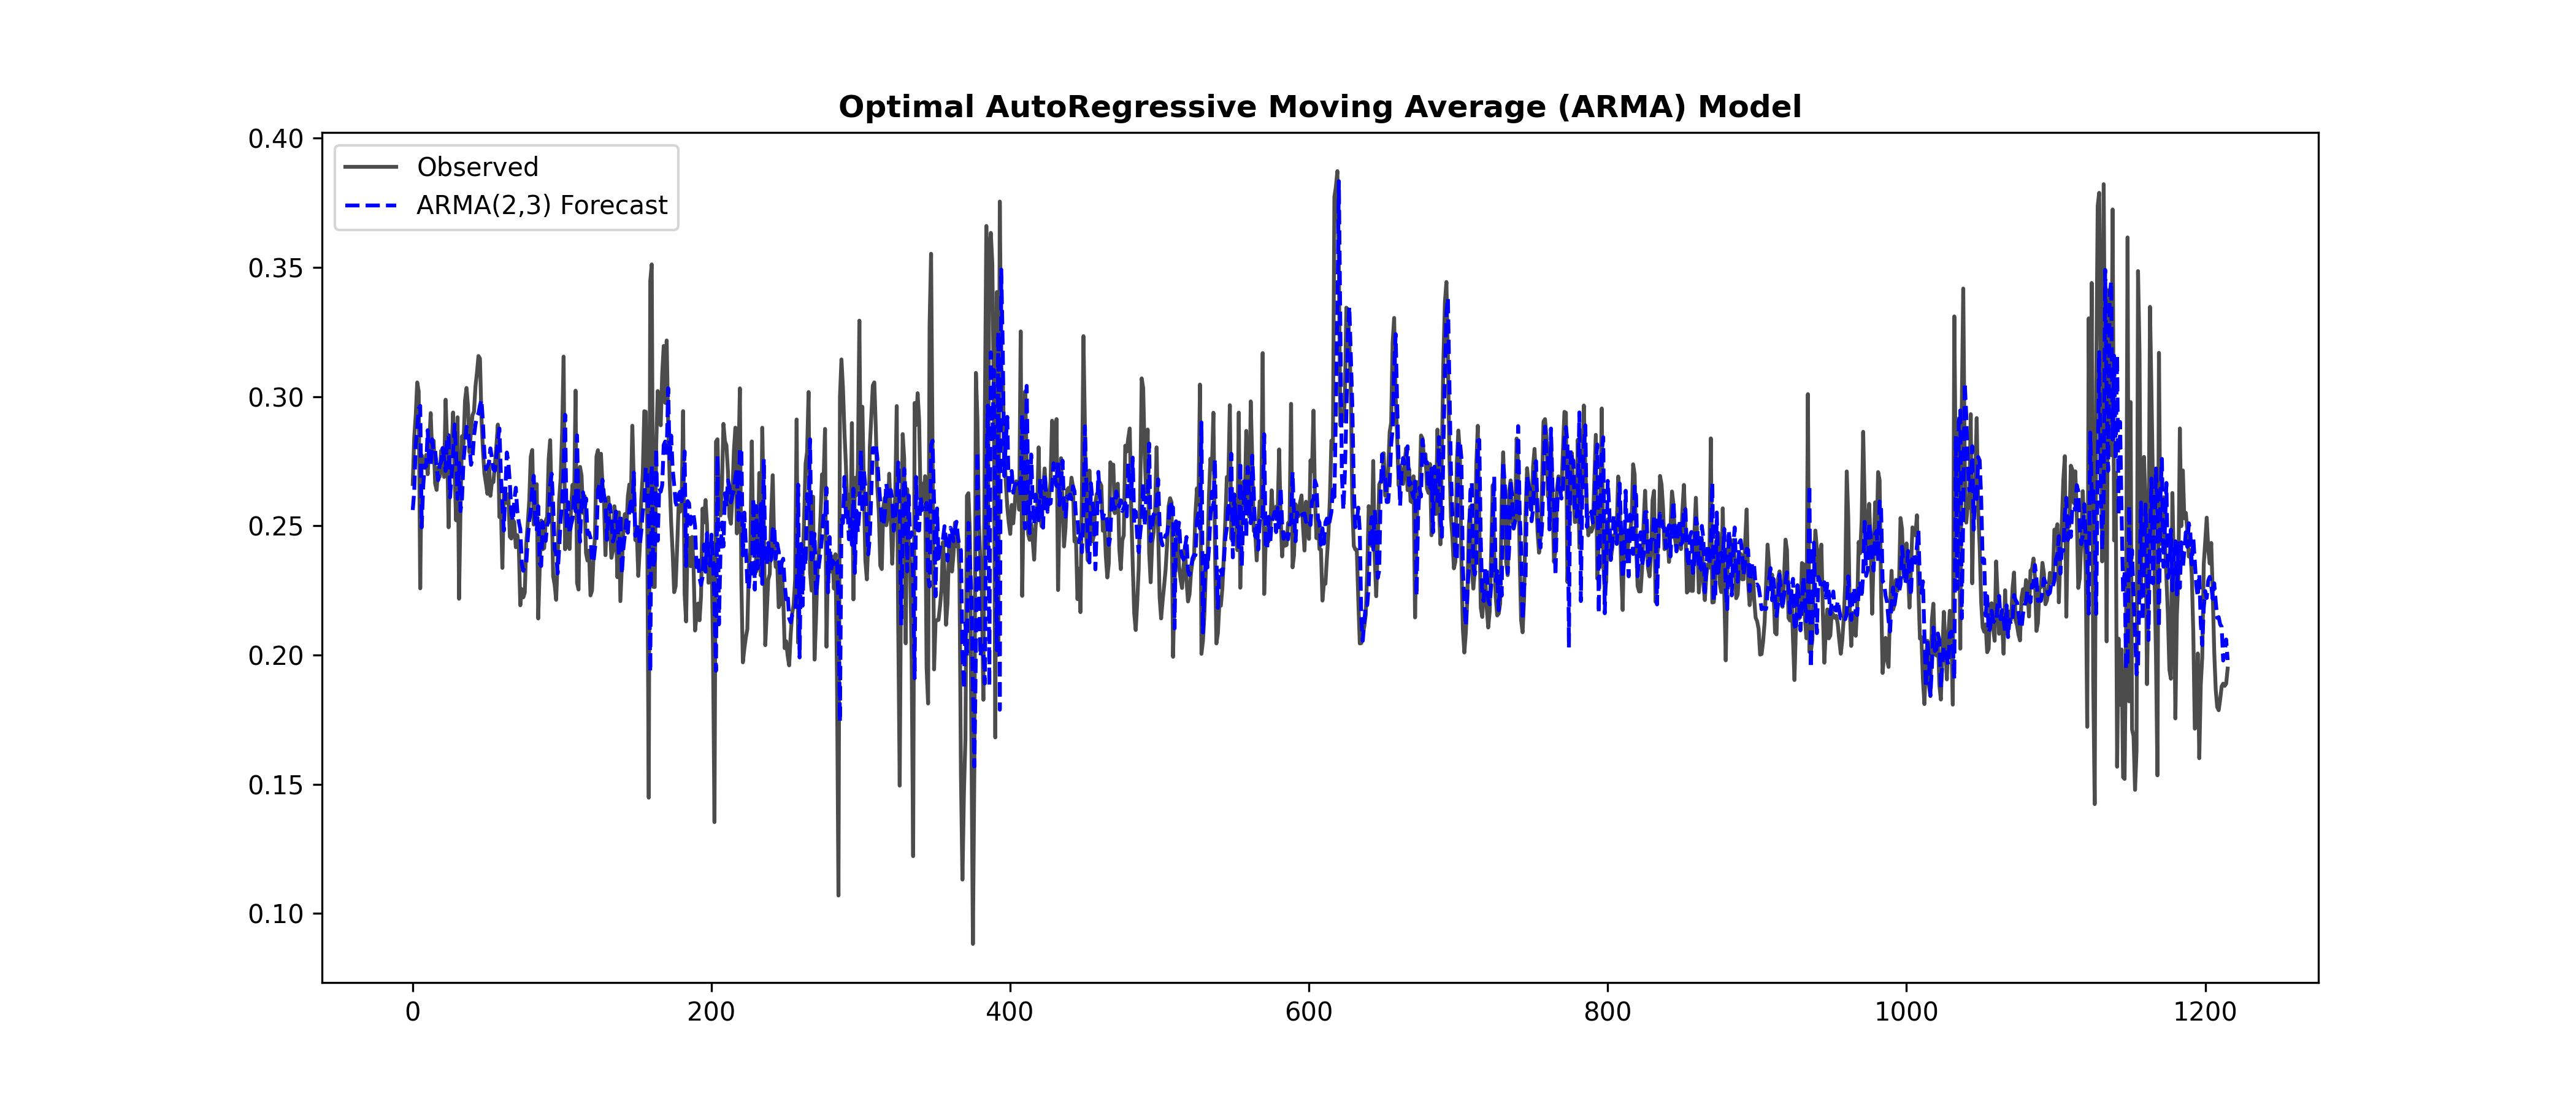
\includegraphics[width=\textwidth, height=0.7\textheight, keepaspectratio]{Forecasting_Graphs/05_ARMA_Optimized.png} \end{column}
        \begin{column}{0.33\textwidth} \metricwidget{ARMA(2,3)}{0.0206}{0.0316}{8.60}{0.2204} \end{column}
    \end{columns}
\end{frame}

% 6. SARIMA
\begin{frame}{Model 6 Theory: SARIMA}
    \textbf{\textcolor{VibrantAmber}{Theoretical Foundation}}
    Adds seasonality $s=7$ to ARIMA to capture repeating physiological rhythms.
    \vspace{0.3cm}
    \begin{tcolorbox}[colback=Midnight!5, colframe=Midnight, title=\textbf{Note}]
        Captures cyclical respiration patterns that affect long-term stress stability.
    \end{tcolorbox}
\end{frame}
\begin{frame}{Model 6 Result: SARIMA}
    \begin{columns}
        \begin{column}{0.65\textwidth} 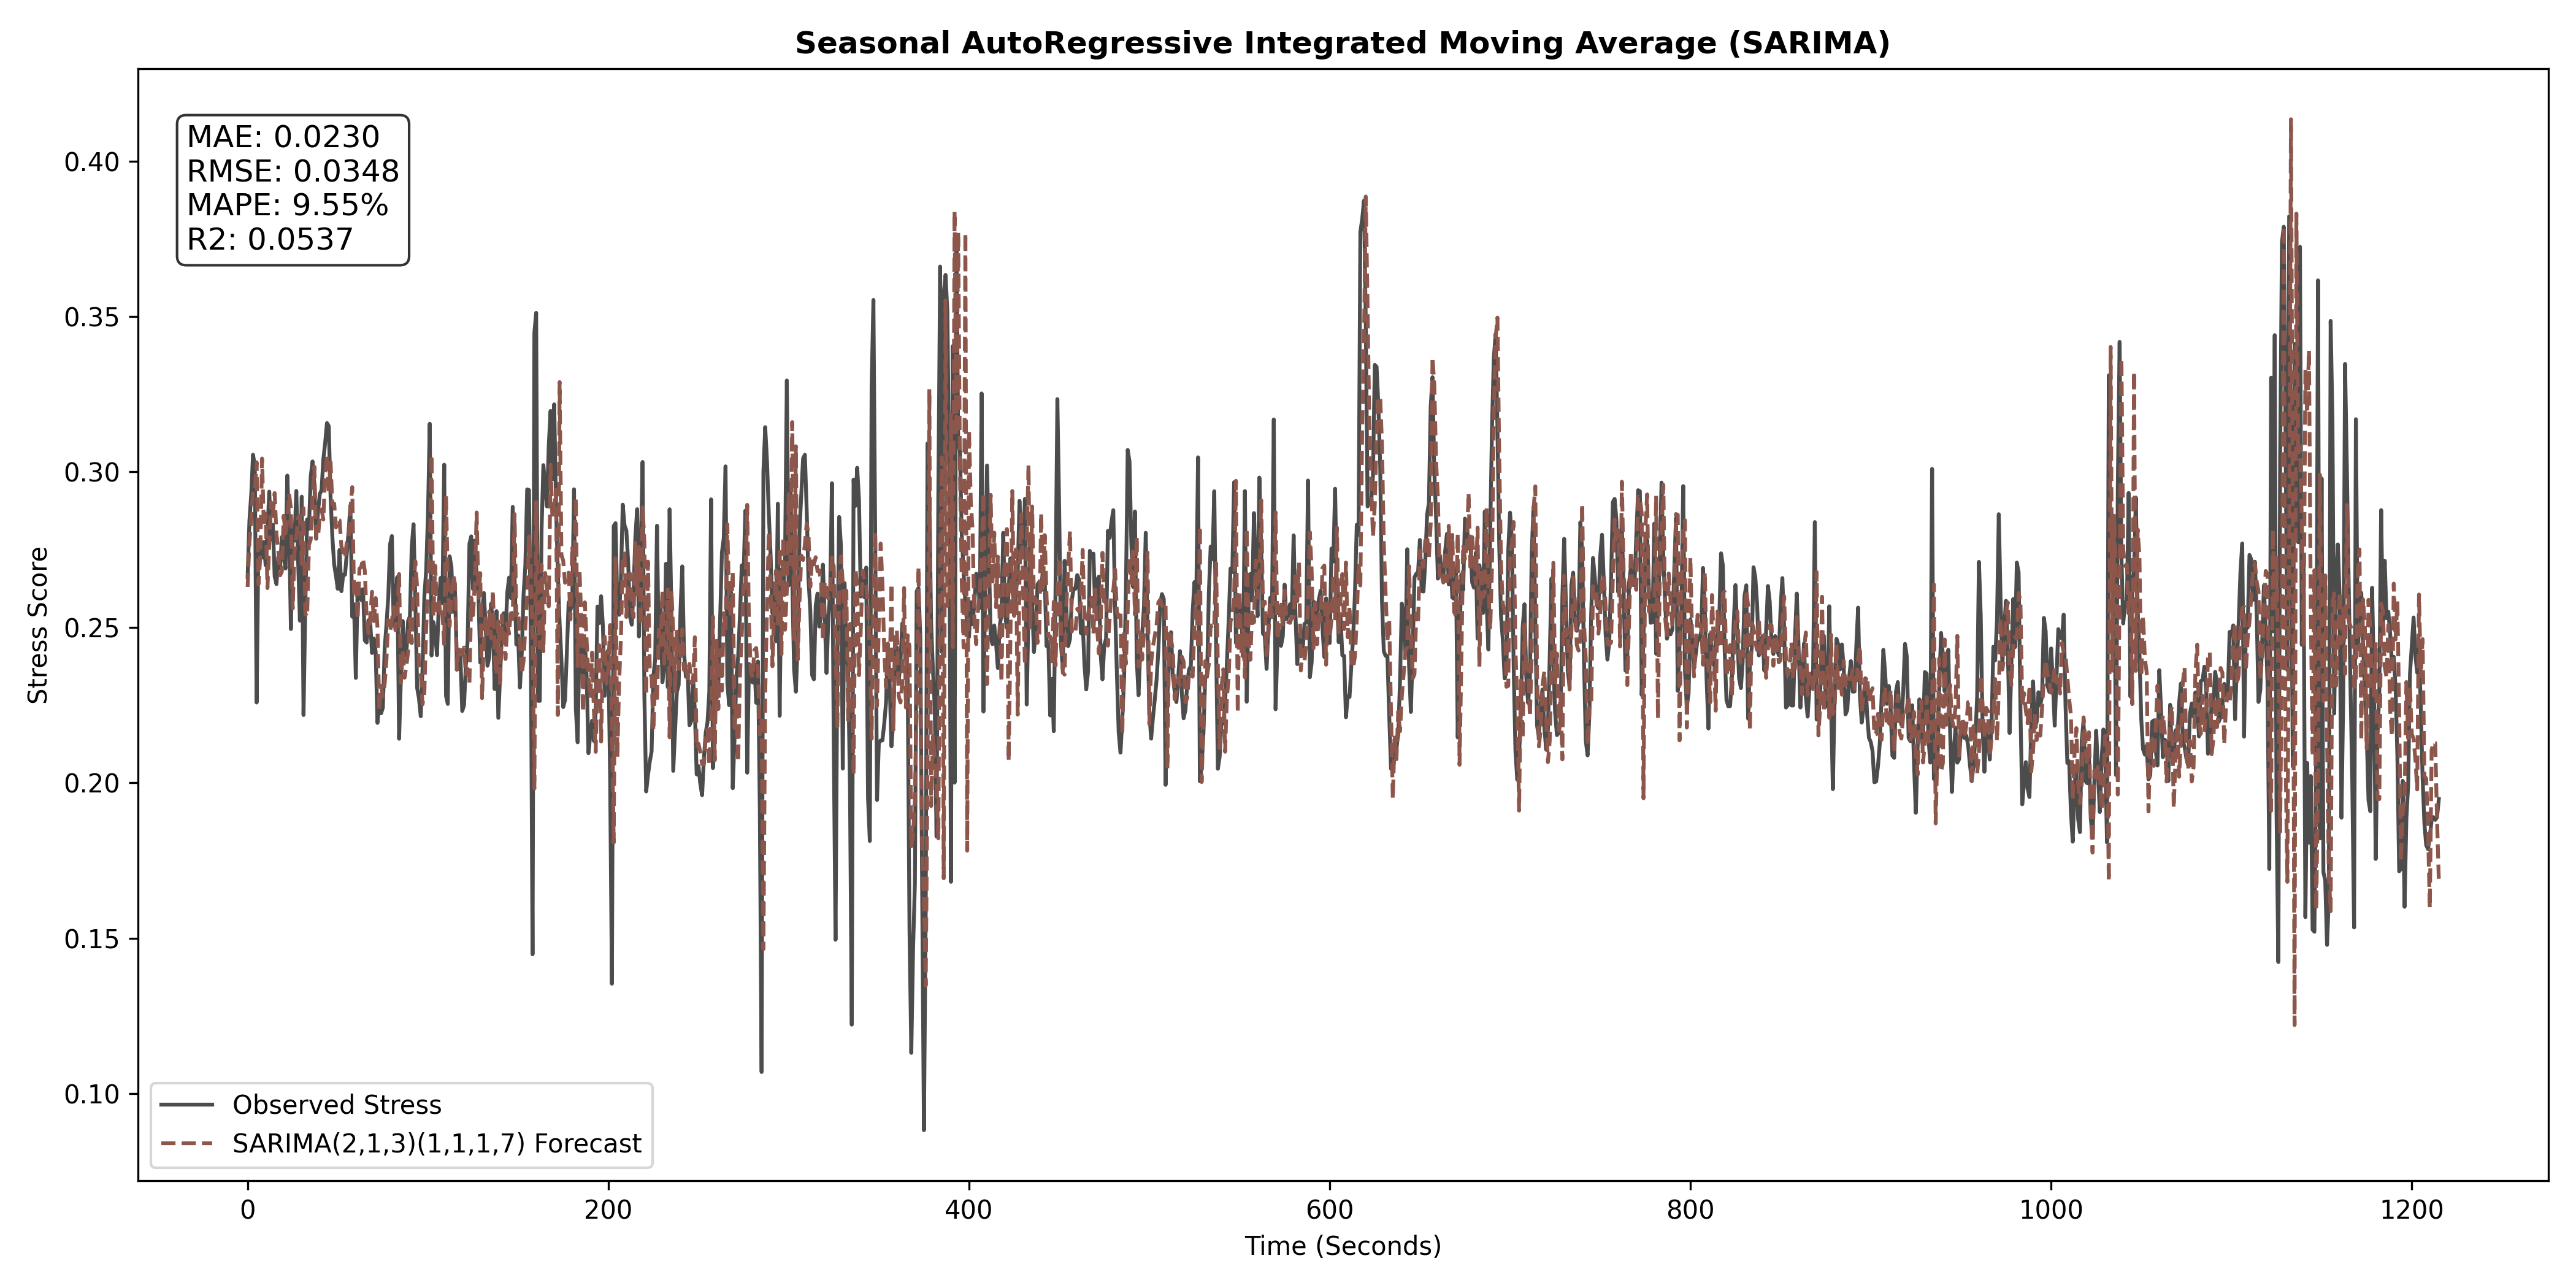
\includegraphics[width=\textwidth, height=0.7\textheight, keepaspectratio]{Forecasting_Graphs/06_SARIMA_Optimized.png} \end{column}
        \begin{column}{0.33\textwidth} \metricwidget{SARIMA}{0.0230}{0.0348}{9.55}{0.0537} \end{column}
    \end{columns}
\end{frame}

% 7. SARIMAX
\begin{frame}{Model 7 Theory: SARIMAX}
    \textbf{\textcolor{VibrantAmber}{Theoretical Foundation}}
    Statistical model incorporating lagged EDA, HR, and TEMP directly into the equation.
    \vspace{0.3cm}
    \begin{tcolorbox}[colback=Midnight!5, colframe=Midnight, title=\textbf{Note}]
        $\hat{y}_t = \text{SARIMA}_t + \boldsymbol{\beta} \mathbf{X}_{t-1}$
    \end{tcolorbox}
\end{frame}
\begin{frame}{Model 7 Result: SARIMAX}
    \begin{columns}
        \begin{column}{0.65\textwidth} 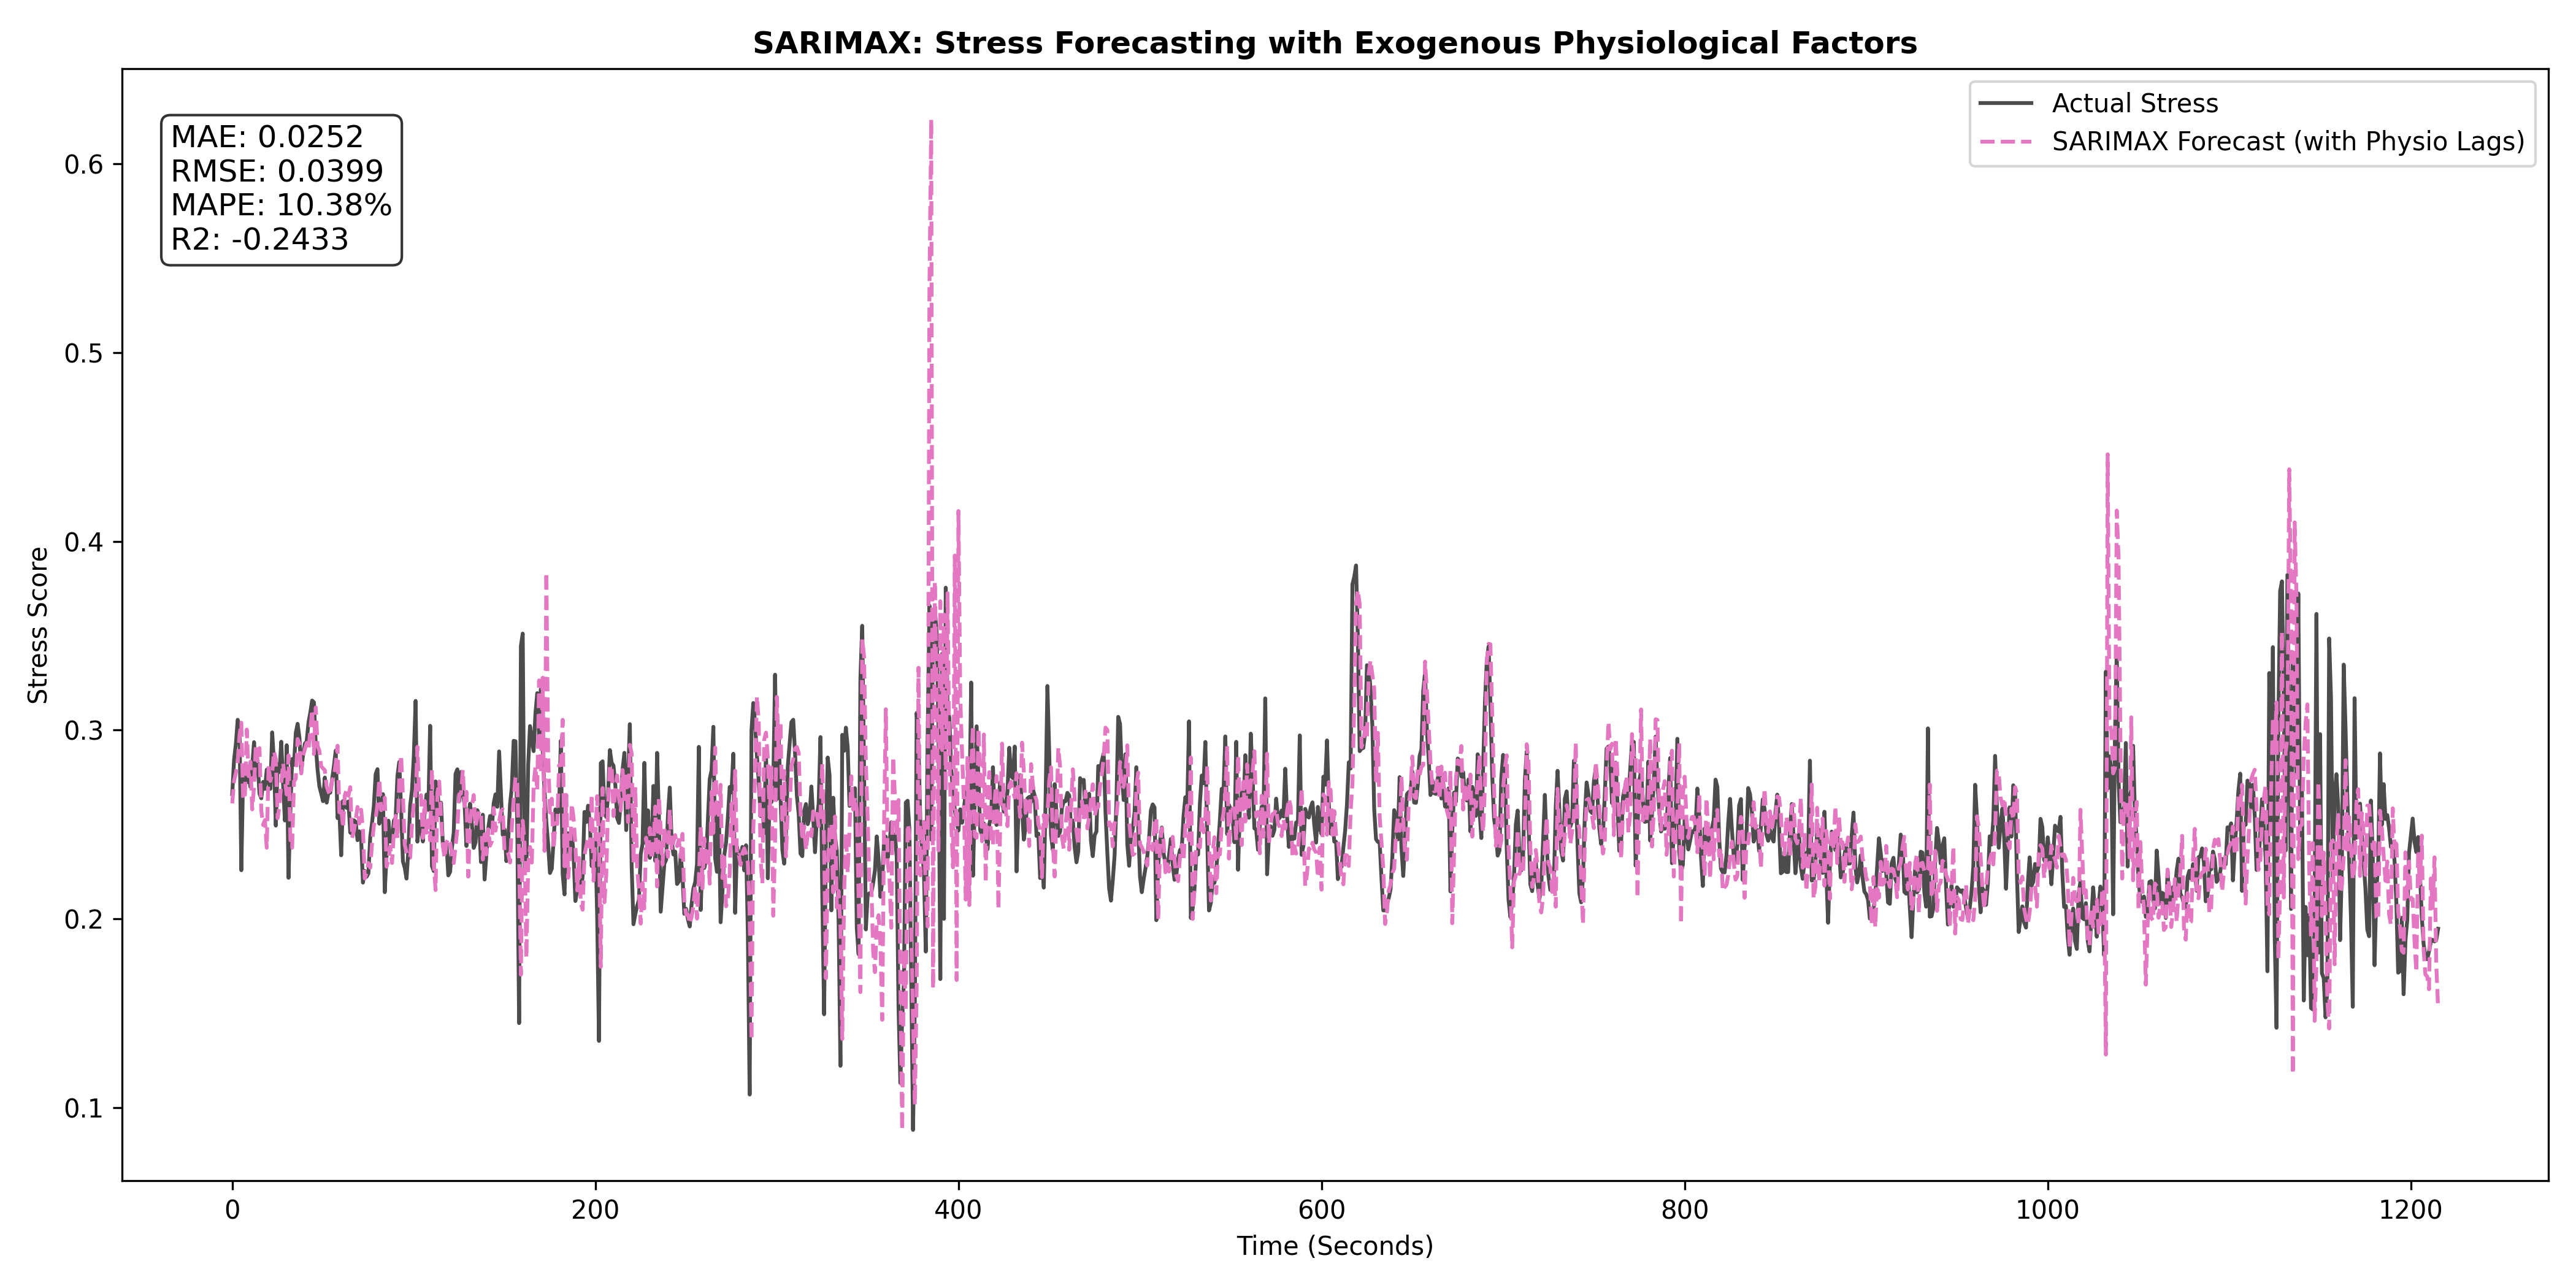
\includegraphics[width=\textwidth, height=0.7\textheight, keepaspectratio]{Forecasting_Graphs/07_SARIMAX_Optimized.png} \end{column}
        \begin{column}{0.33\textwidth} \metricwidget{SARIMAX}{0.0252}{0.0399}{10.38}{-0.2433} \end{column}
    \end{columns}
\end{frame}

% 8. RF
\begin{frame}{Model 8 Theory: Random Forest}
    \textbf{\textcolor{VibrantAmber}{Theoretical Foundation}}
    Ensemble of 100 decision trees. Non-parametric approach to sensor noise.
    \vspace{0.3cm}
    \begin{tcolorbox}[colback=Midnight!5, colframe=Midnight, title=\textbf{Approach}]
        Handles non-linear feature interactions without needing differencing.
    \end{tcolorbox}
\end{frame}
\begin{frame}{Model 8 Result: Random Forest}
    \begin{columns}
        \begin{column}{0.65\textwidth} 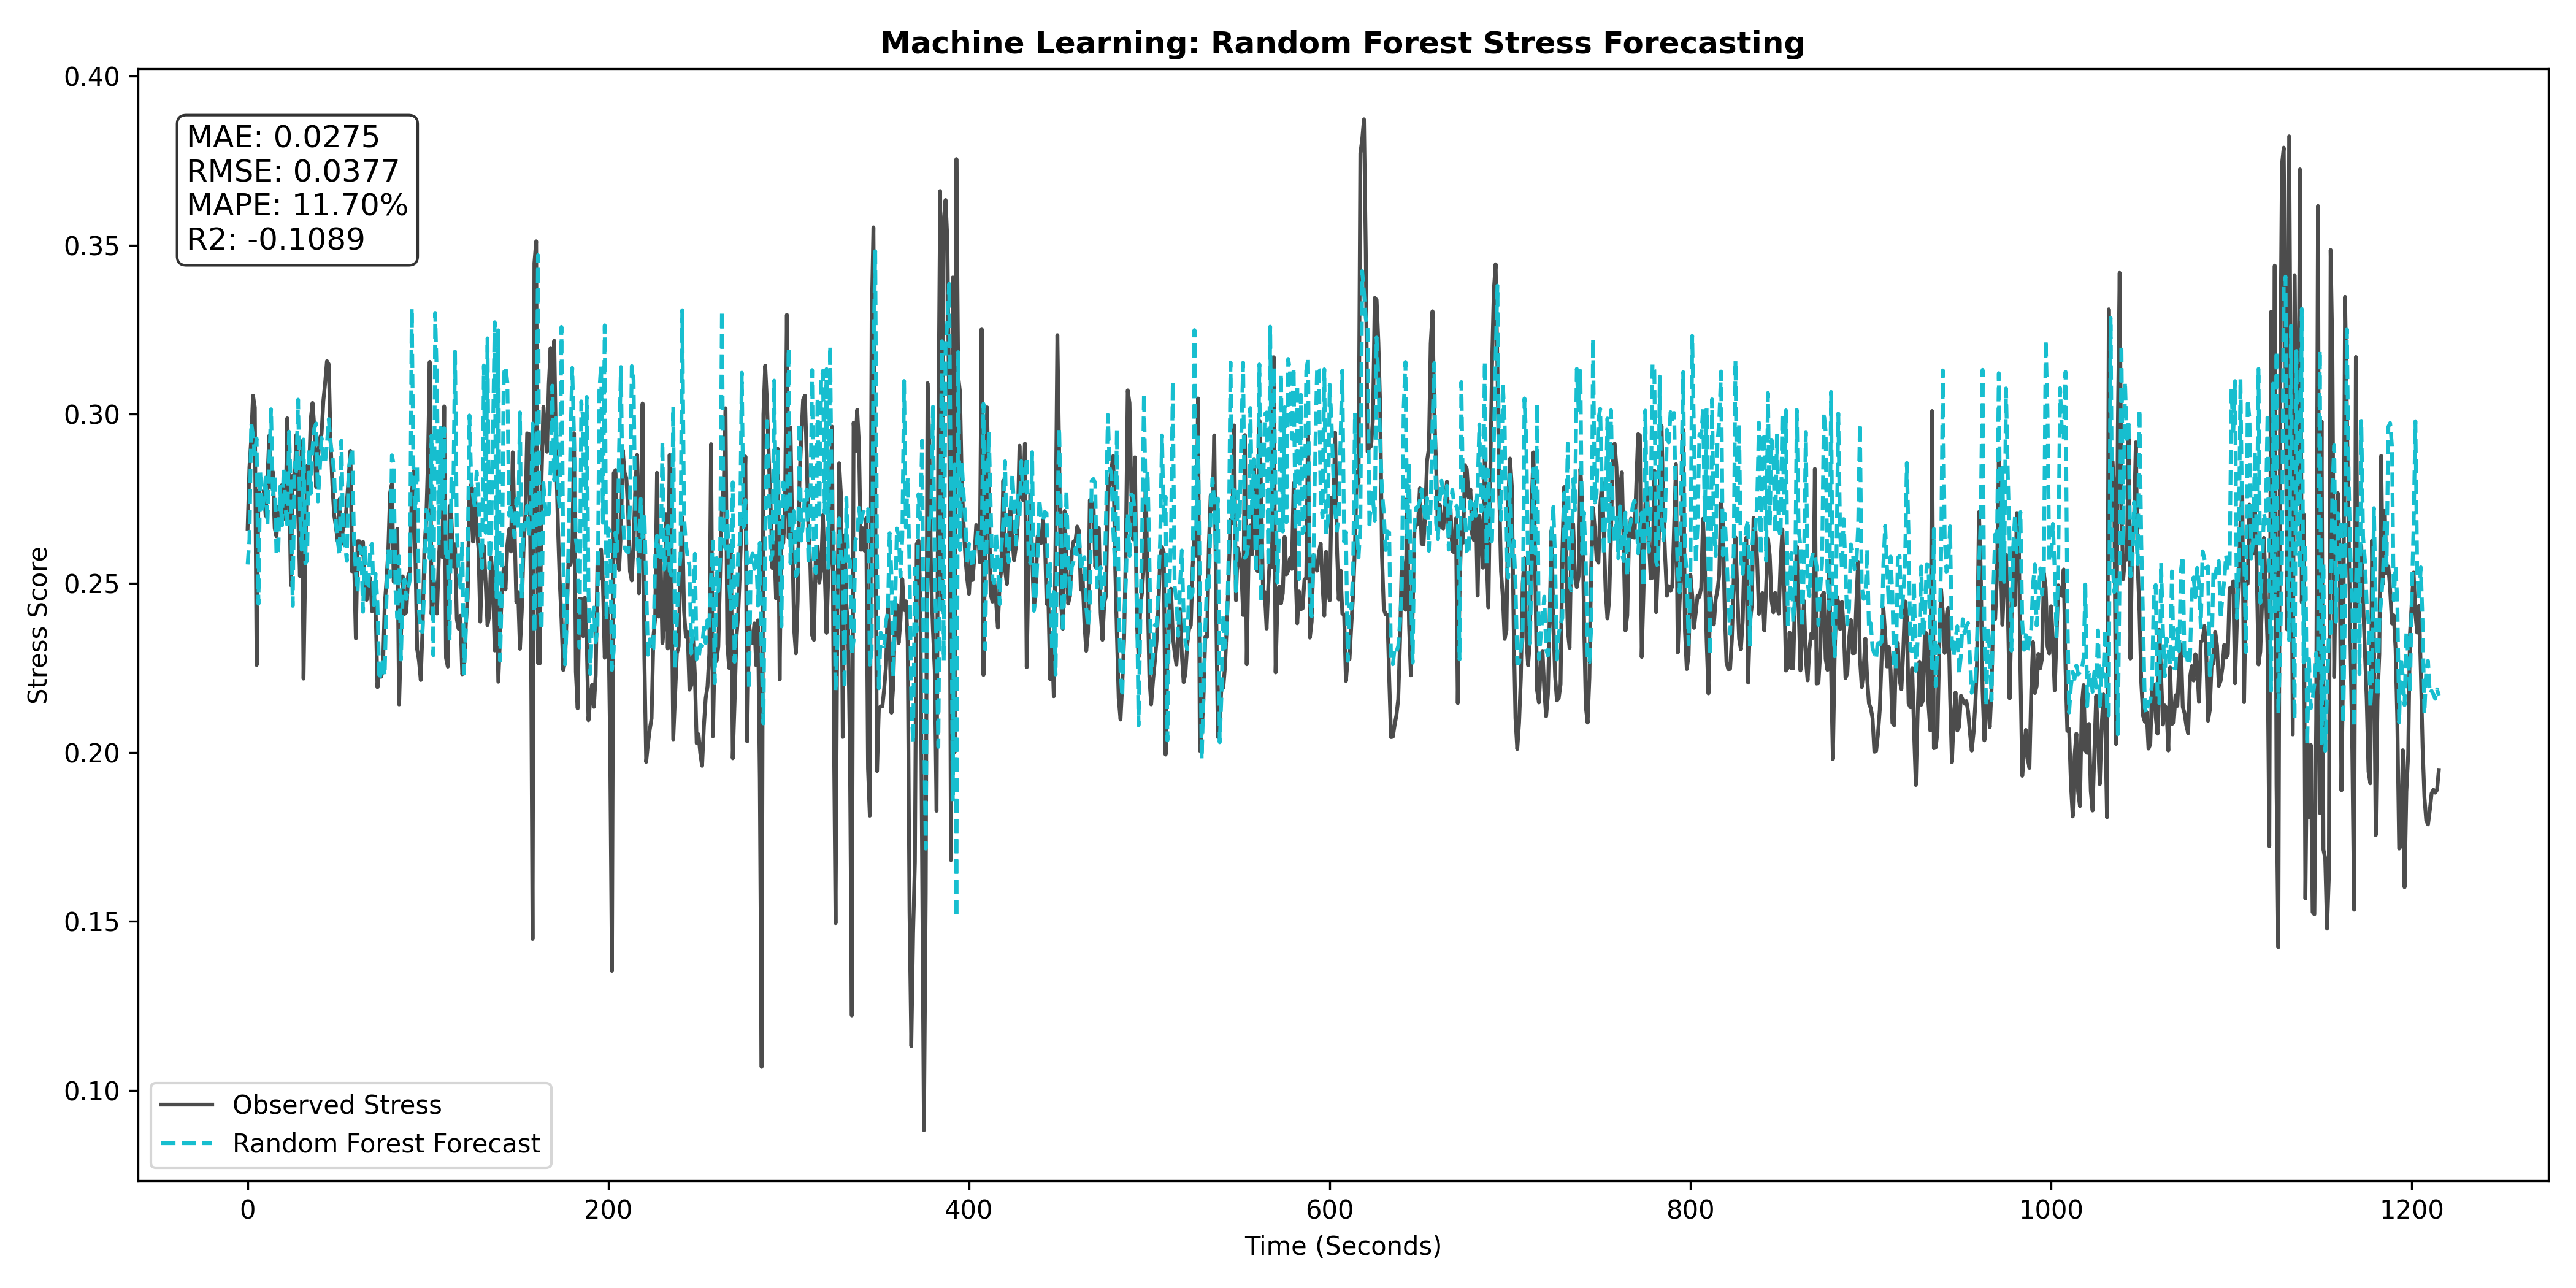
\includegraphics[width=\textwidth, height=0.7\textheight, keepaspectratio]{Forecasting_Graphs/08_Random_Forest_Forecast.png} \end{column}
        \begin{column}{0.33\textwidth} \metricwidget{RF}{0.0275}{0.0377}{11.70}{-0.1089} \end{column}
    \end{columns}
\end{frame}

% 9. XGBoost
\begin{frame}{Model 9 Theory: XGBoost}
    \textbf{\textcolor{VibrantAmber}{Theoretical Foundation}}
    Extreme Gradient Boosting. Sequentially minimizes errors of previous trees.
    \vspace{0.3cm}
    \begin{tcolorbox}[colback=Midnight!5, colframe=Midnight, title=\textbf{Advantage}]
        State-of-the-art for high-frequency tabular signal forecasting.
    \end{tcolorbox}
\end{frame}
\begin{frame}{Model 9 Result: XGBoost}
    \begin{columns}
        \begin{column}{0.65\textwidth} 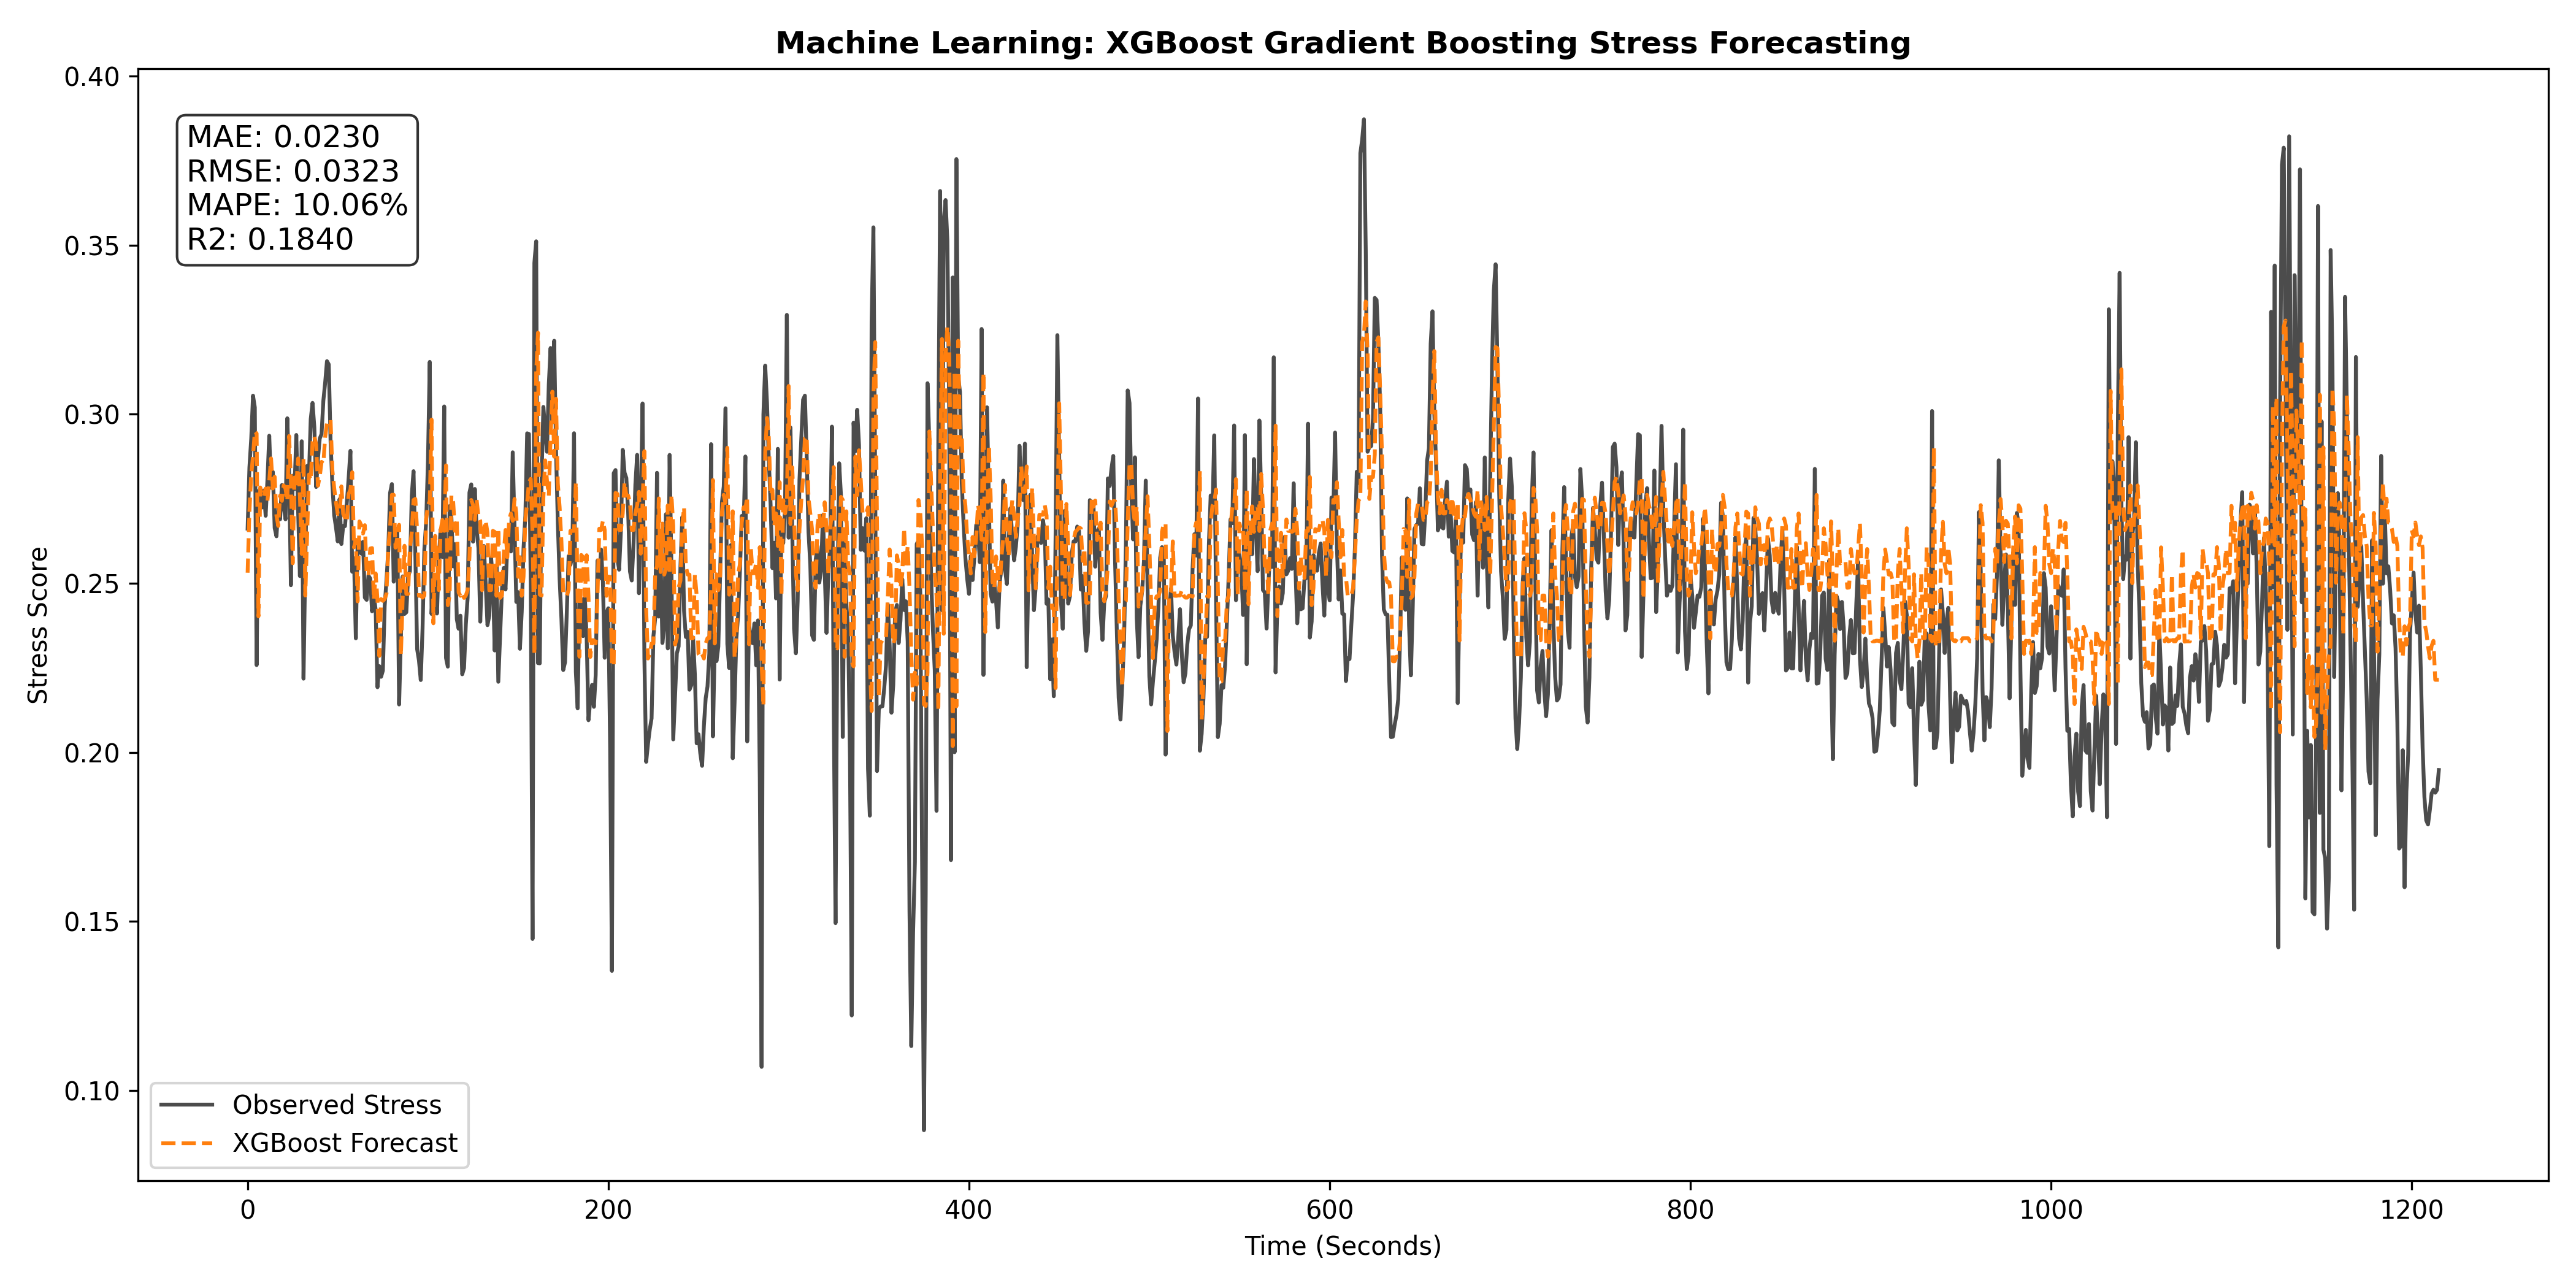
\includegraphics[width=\textwidth, height=0.7\textheight, keepaspectratio]{Forecasting_Graphs/09_XGBoost_Forecast.png} \end{column}
        \begin{column}{0.33\textwidth} \metricwidget{XGBoost}{0.0230}{0.0323}{10.06}{0.1840} \end{column}
    \end{columns}
\end{frame}

% 10. LSTM
\begin{frame}{Model 10 Theory: LSTM}
    \textbf{\textcolor{VibrantAmber}{Theoretical Foundation}}
    Long Short-Term Memory. Recurrent gates maintain a 10s temporal window.
    \vspace{0.3cm}
    \begin{tcolorbox}[colback=Midnight!5, colframe=Midnight, title=\textbf{Note}]
        Captures sequential dependencies that tree-based models miss.
    \end{tcolorbox}
\end{frame}
\begin{frame}{Model 10 Result: LSTM}
    \begin{columns}
        \begin{column}{0.65\textwidth} 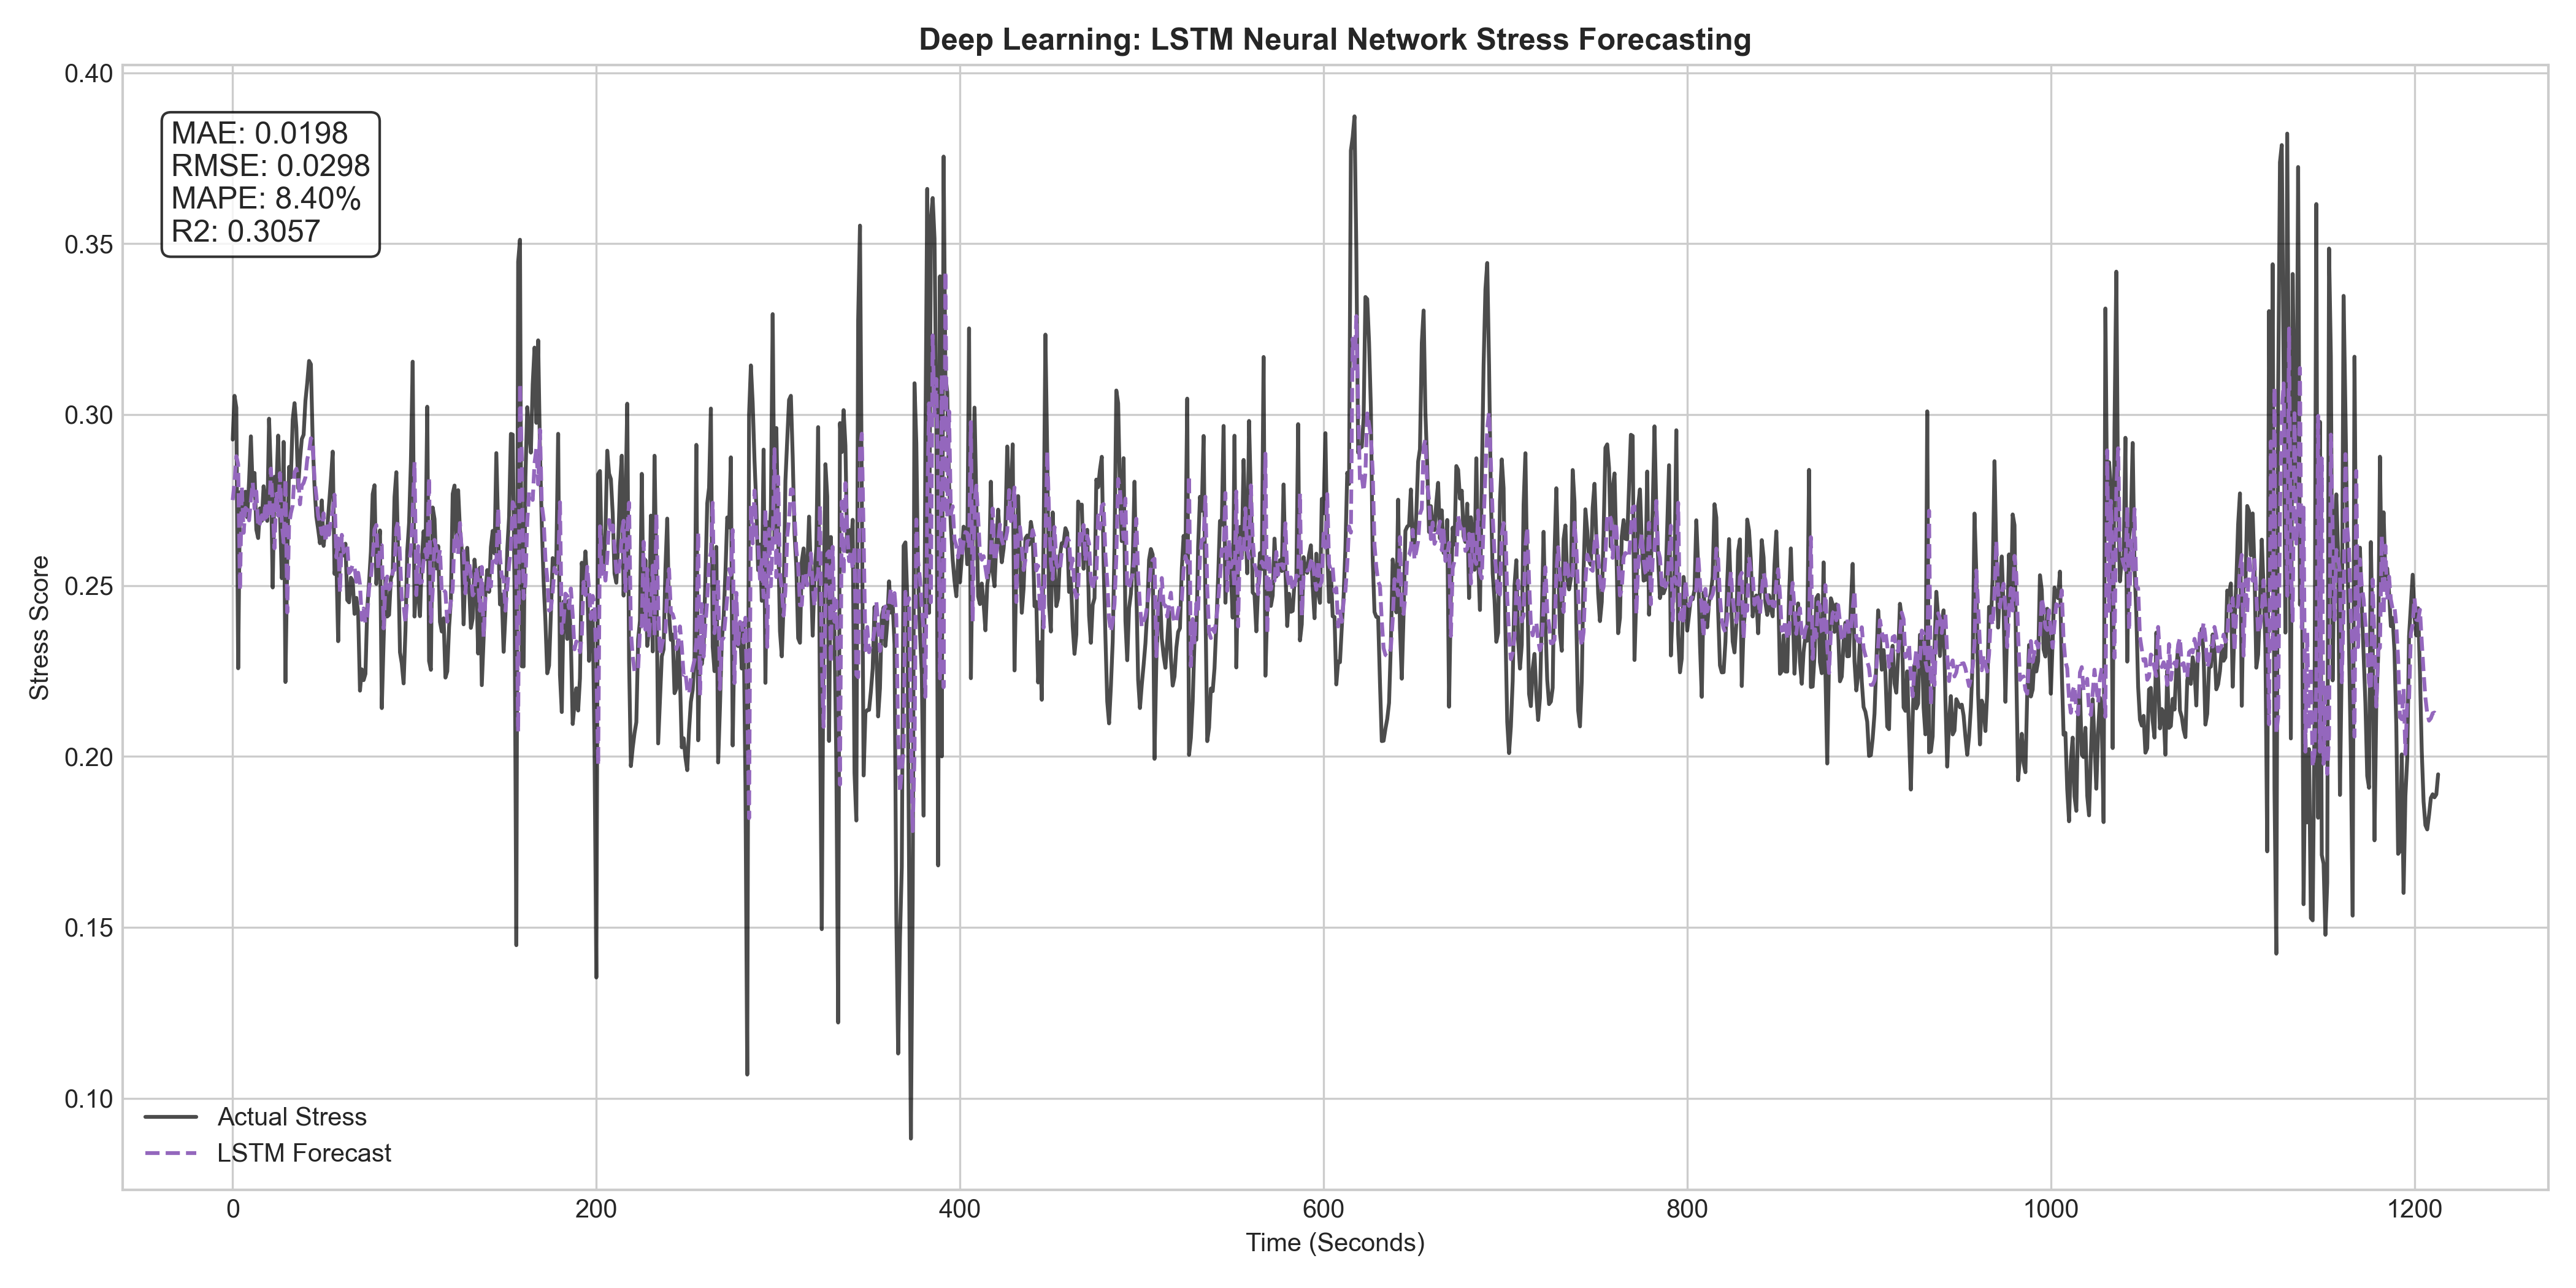
\includegraphics[width=\textwidth, height=0.7\textheight, keepaspectratio]{Forecasting_Graphs/10_LSTM_Forecast.png} \end{column}
        \begin{column}{0.33\textwidth} \metricwidget{LSTM}{0.0198}{0.0298}{8.40}{0.3057} \end{column}
    \end{columns}
\end{frame}

% 11. SVR
\begin{frame}{Model 11 Theory: SVR}
    \textbf{\textcolor{VibrantAmber}{Theoretical Foundation}}
    Support Vector Regression using RBF kernels for high-dimensional margins.
    \vspace{0.3cm}
    \begin{tcolorbox}[colback=Midnight!5, colframe=Midnight, title=\textbf{Logic}]
        Finds non-linear decision boundaries around stress onset zones.
    \end{tcolorbox}
\end{frame}
\begin{frame}{Model 11 Result: SVR}
    \begin{columns}
        \begin{column}{0.65\textwidth} 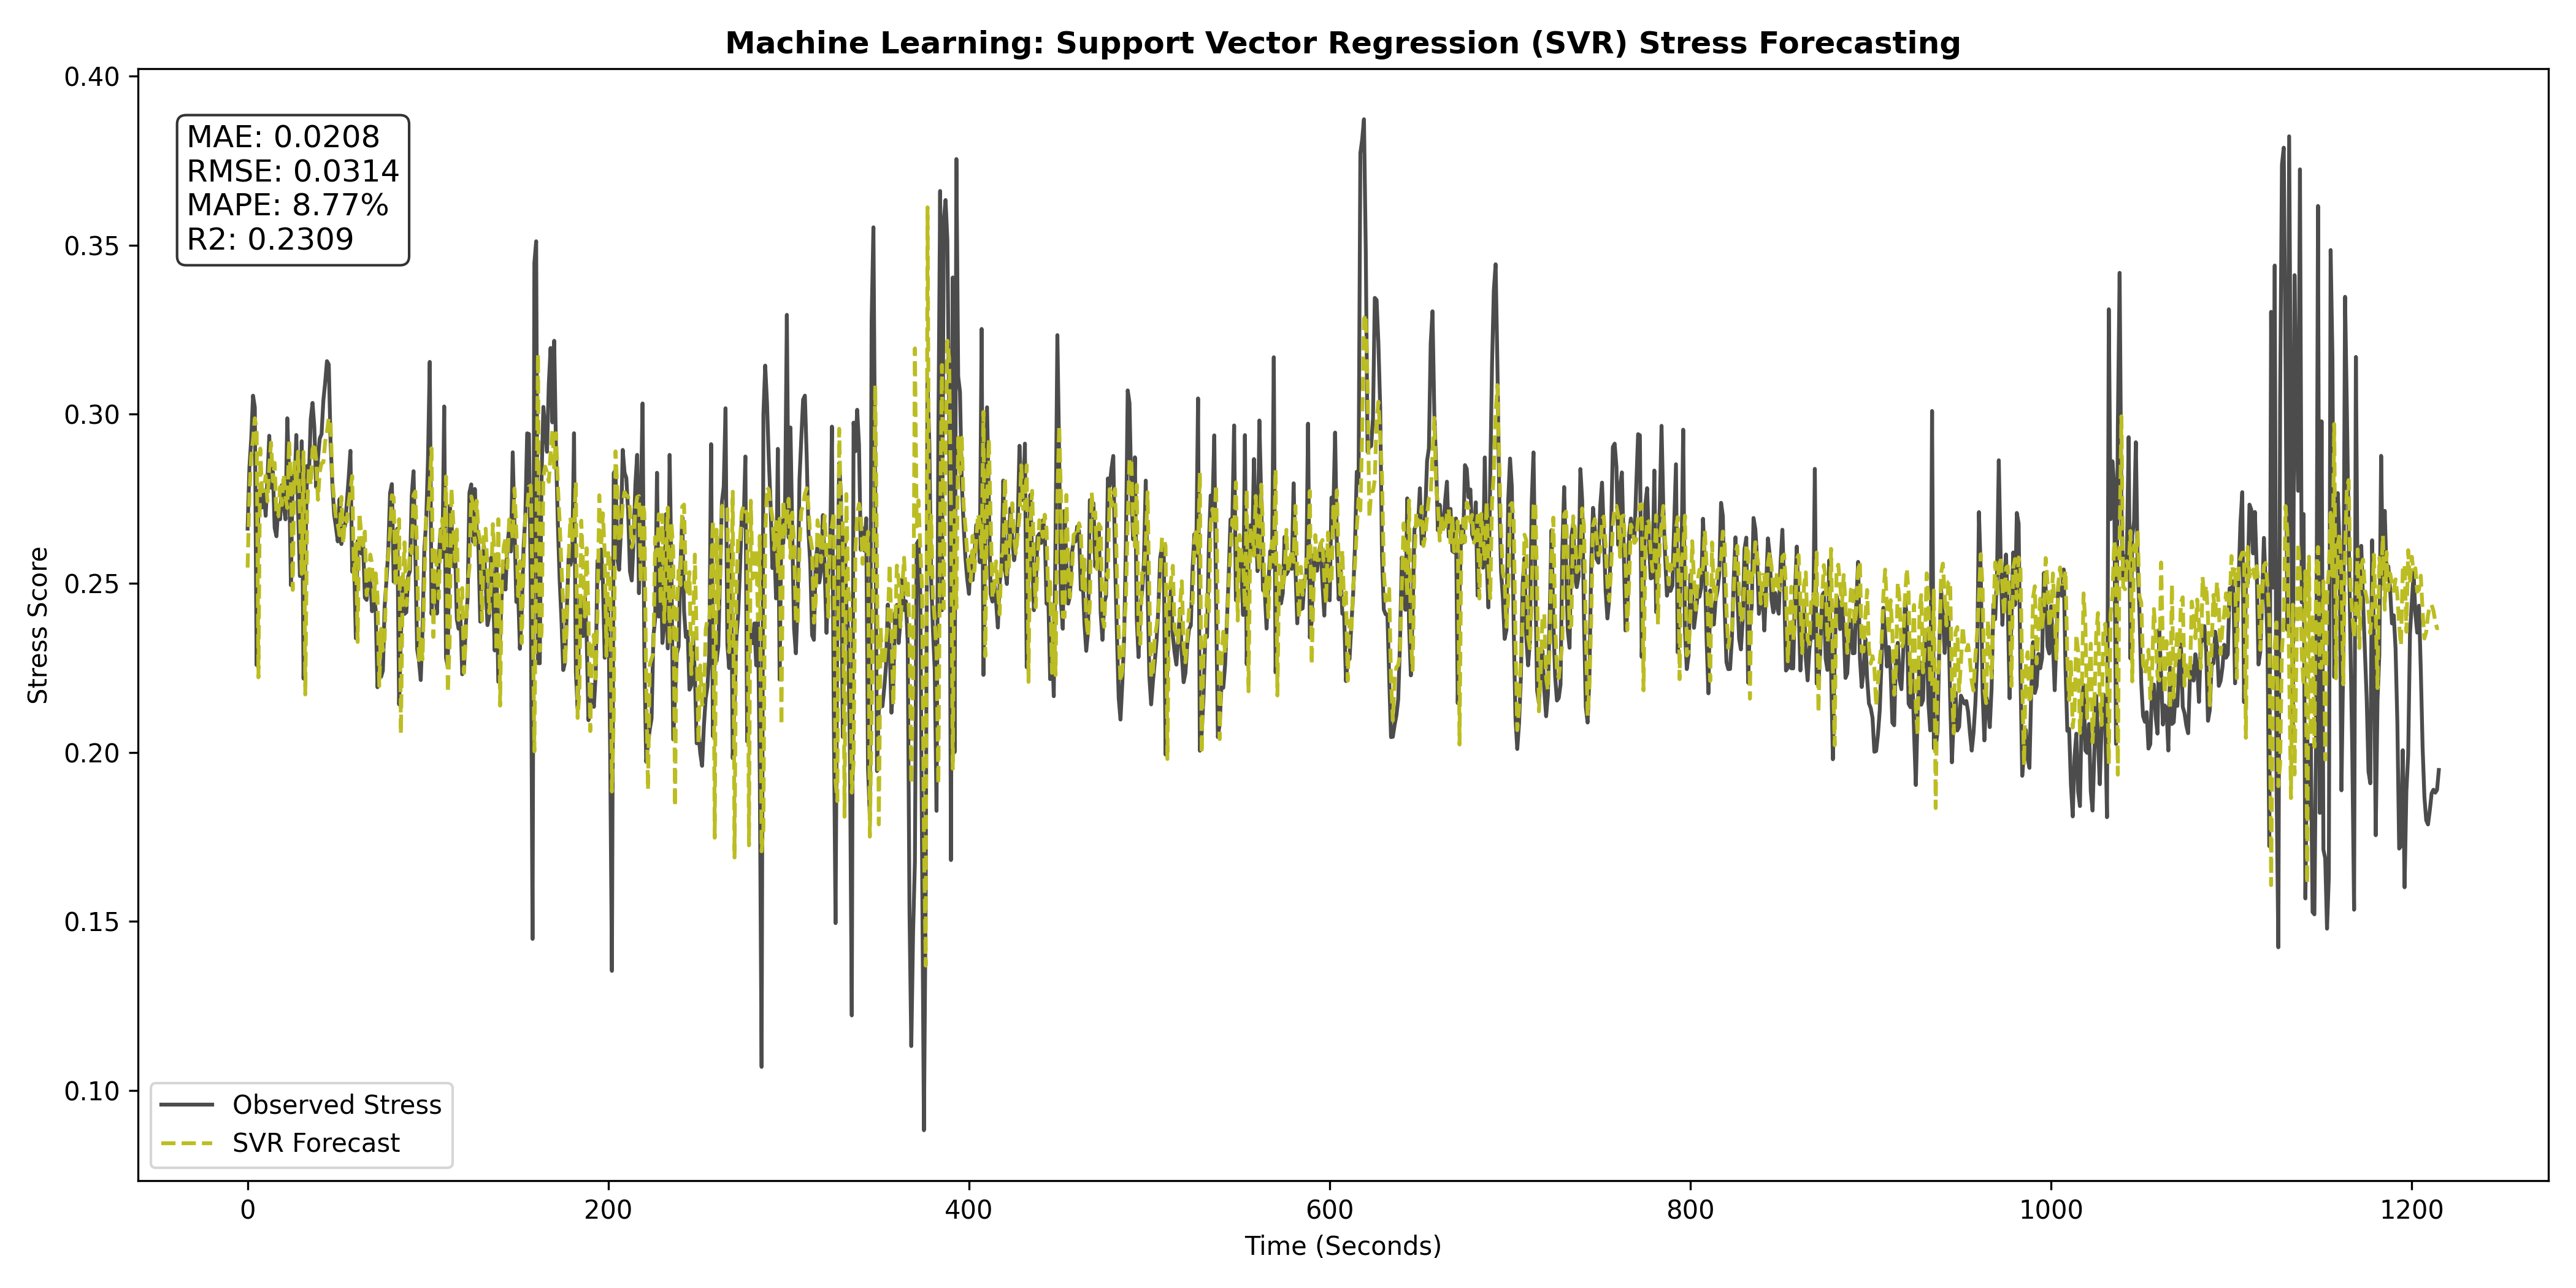
\includegraphics[width=\textwidth, height=0.7\textheight, keepaspectratio]{Forecasting_Graphs/11_SVR_Forecast.png} \end{column}
        \begin{column}{0.33\textwidth} \metricwidget{SVR}{0.0208}{0.0314}{8.77}{0.2309} \end{column}
    \end{columns}
\end{frame}

% 12. GRU
\begin{frame}{Model 12 Theory: GRU}
    \textbf{\textcolor{VibrantAmber}{Theoretical Foundation}}
    Gated Recurrent Unit. Efficient variation of LSTM with fewer parameters.
    \vspace{0.3cm}
    \begin{tcolorbox}[colback=Midnight!5, colframe=Midnight, title=\textbf{Concept}]
        Optimized for high-throughput sensor data processing.
    \end{tcolorbox}
\end{frame}
\begin{frame}{Model 12 Result: GRU}
    \begin{columns}
        \begin{column}{0.65\textwidth} 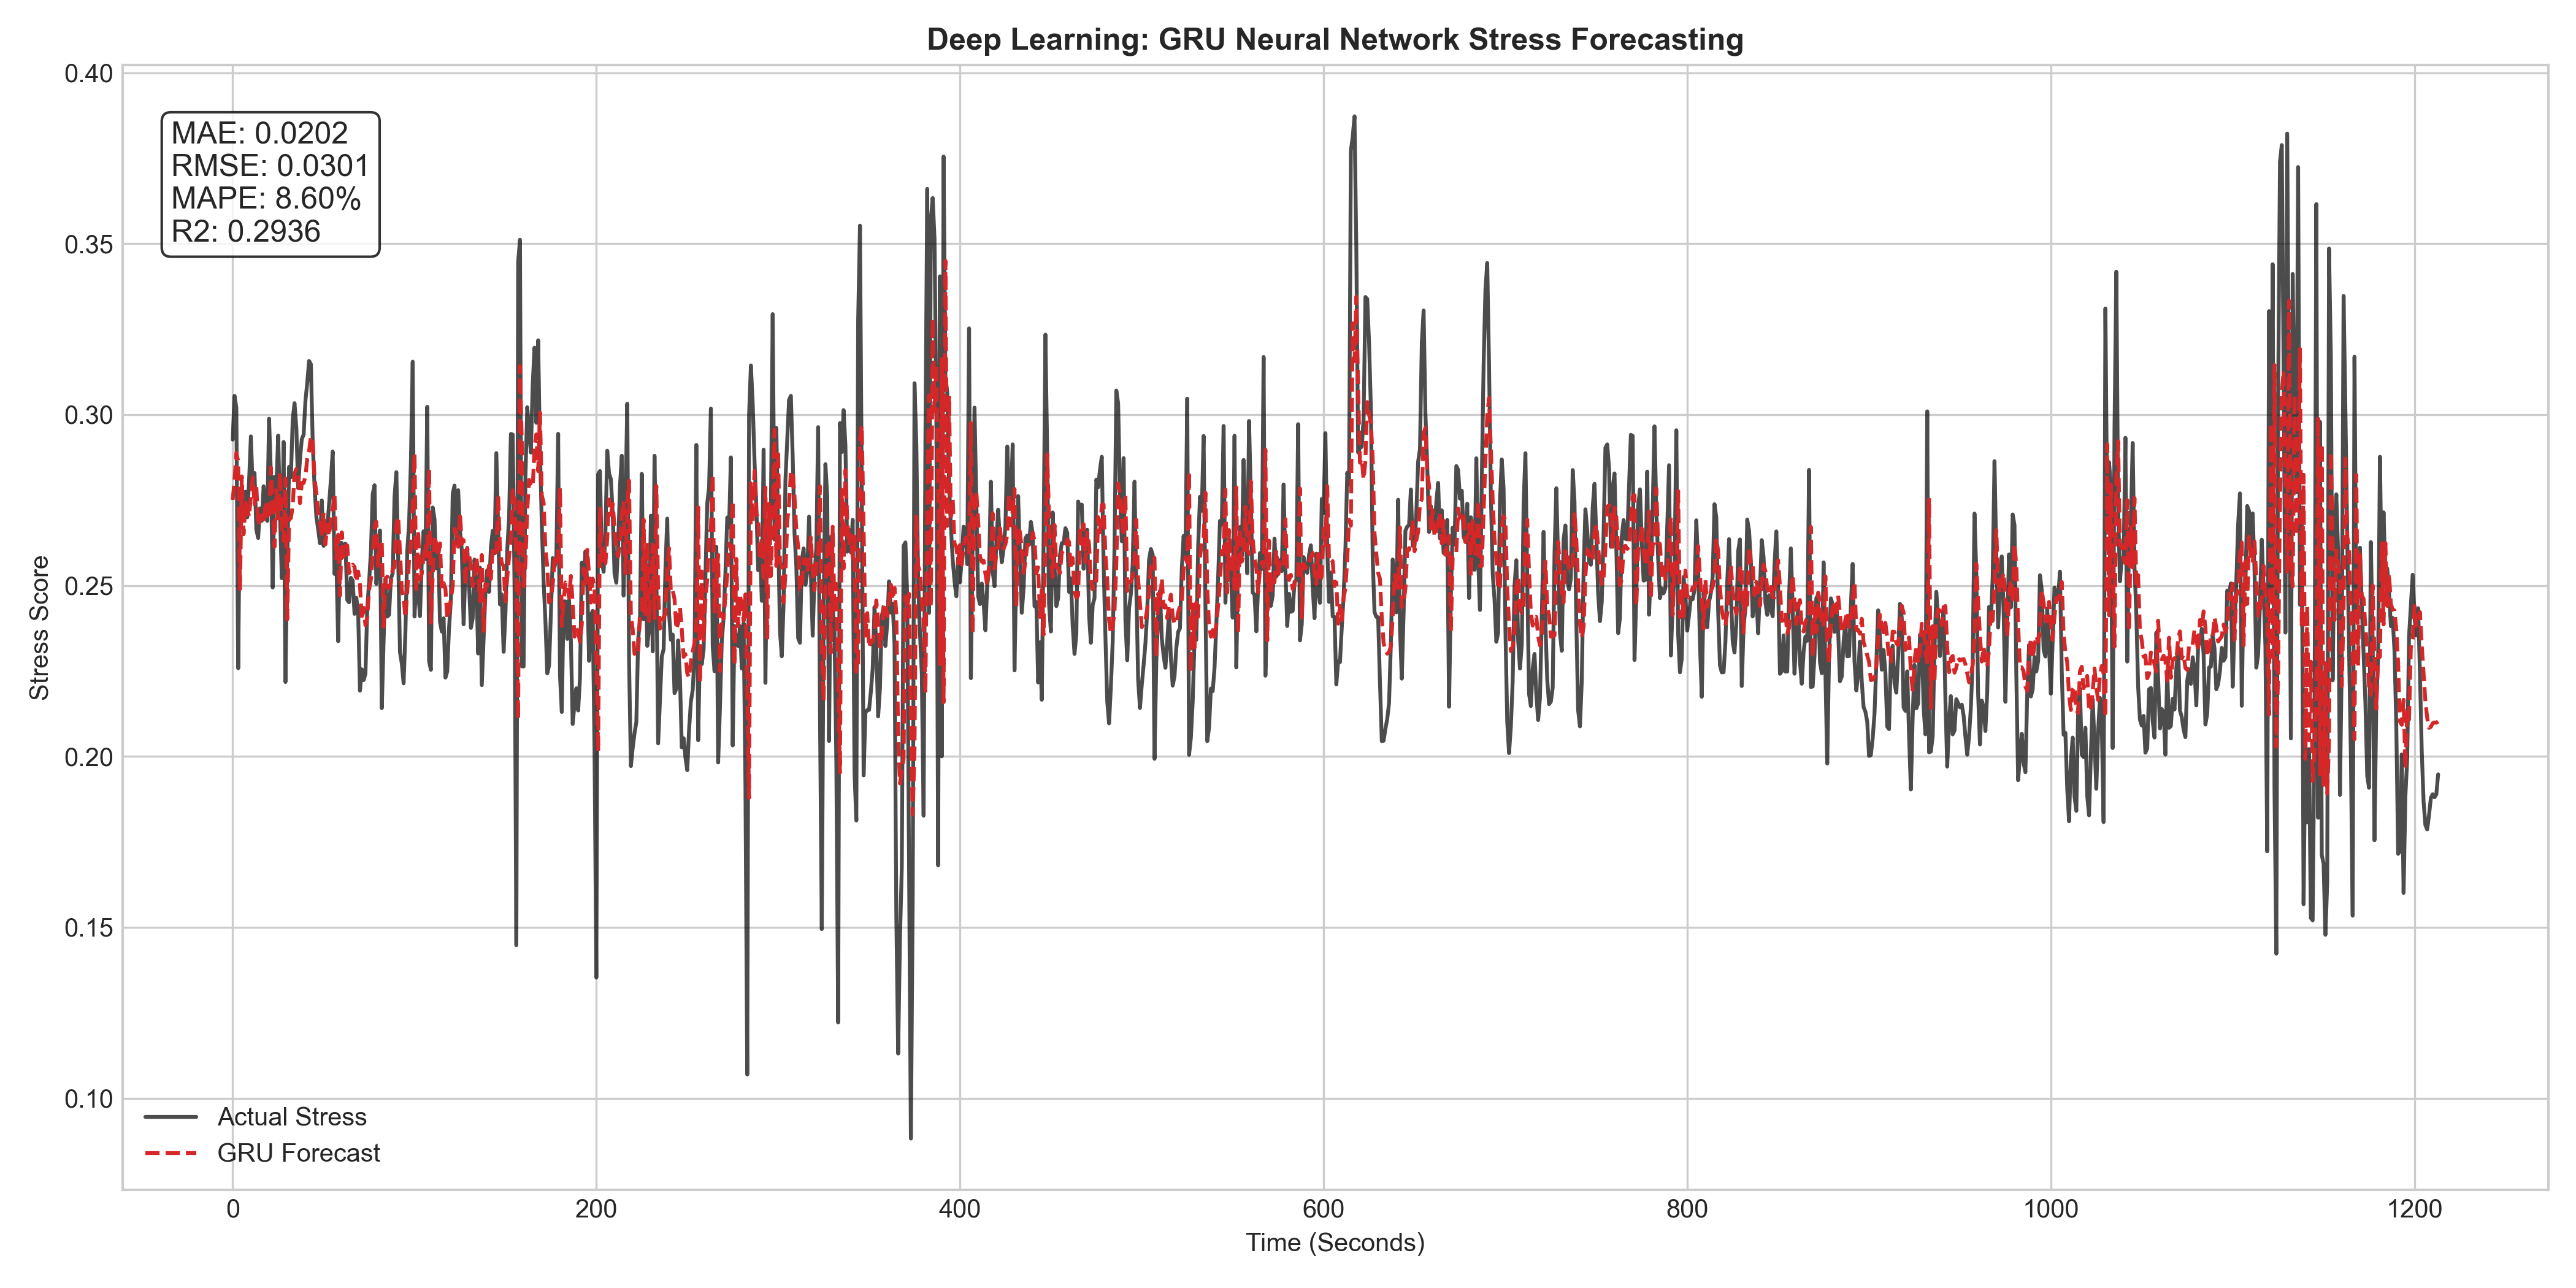
\includegraphics[width=\textwidth, height=0.7\textheight, keepaspectratio]{Forecasting_Graphs/12_GRU_Forecast.png} \end{column}
        \begin{column}{0.33\textwidth} \metricwidget{GRU}{0.0202}{0.0301}{8.60}{0.2936} \end{column}
    \end{columns}
\end{frame}

% 13. Quantile
\begin{frame}{Model 13 Theory: Quantile Regression}
    \textbf{\textcolor{VibrantAmber}{Theoretical Foundation}}
    Risk-bounded forecasting. Optimizes Pinball Loss for specific percentiles.
    \vspace{0.3cm}
    \begin{tcolorbox}[colback=Midnight!5, colframe=Midnight, title=\textbf{Note}]
        Predicts an Upper Risk Boundary (95th Pctl) for clinical safety.
    \end{tcolorbox}
\end{frame}
\begin{frame}{Model 13 Result: Quantile Risk Bounds}
    \begin{columns}
        \begin{column}{0.65\textwidth} 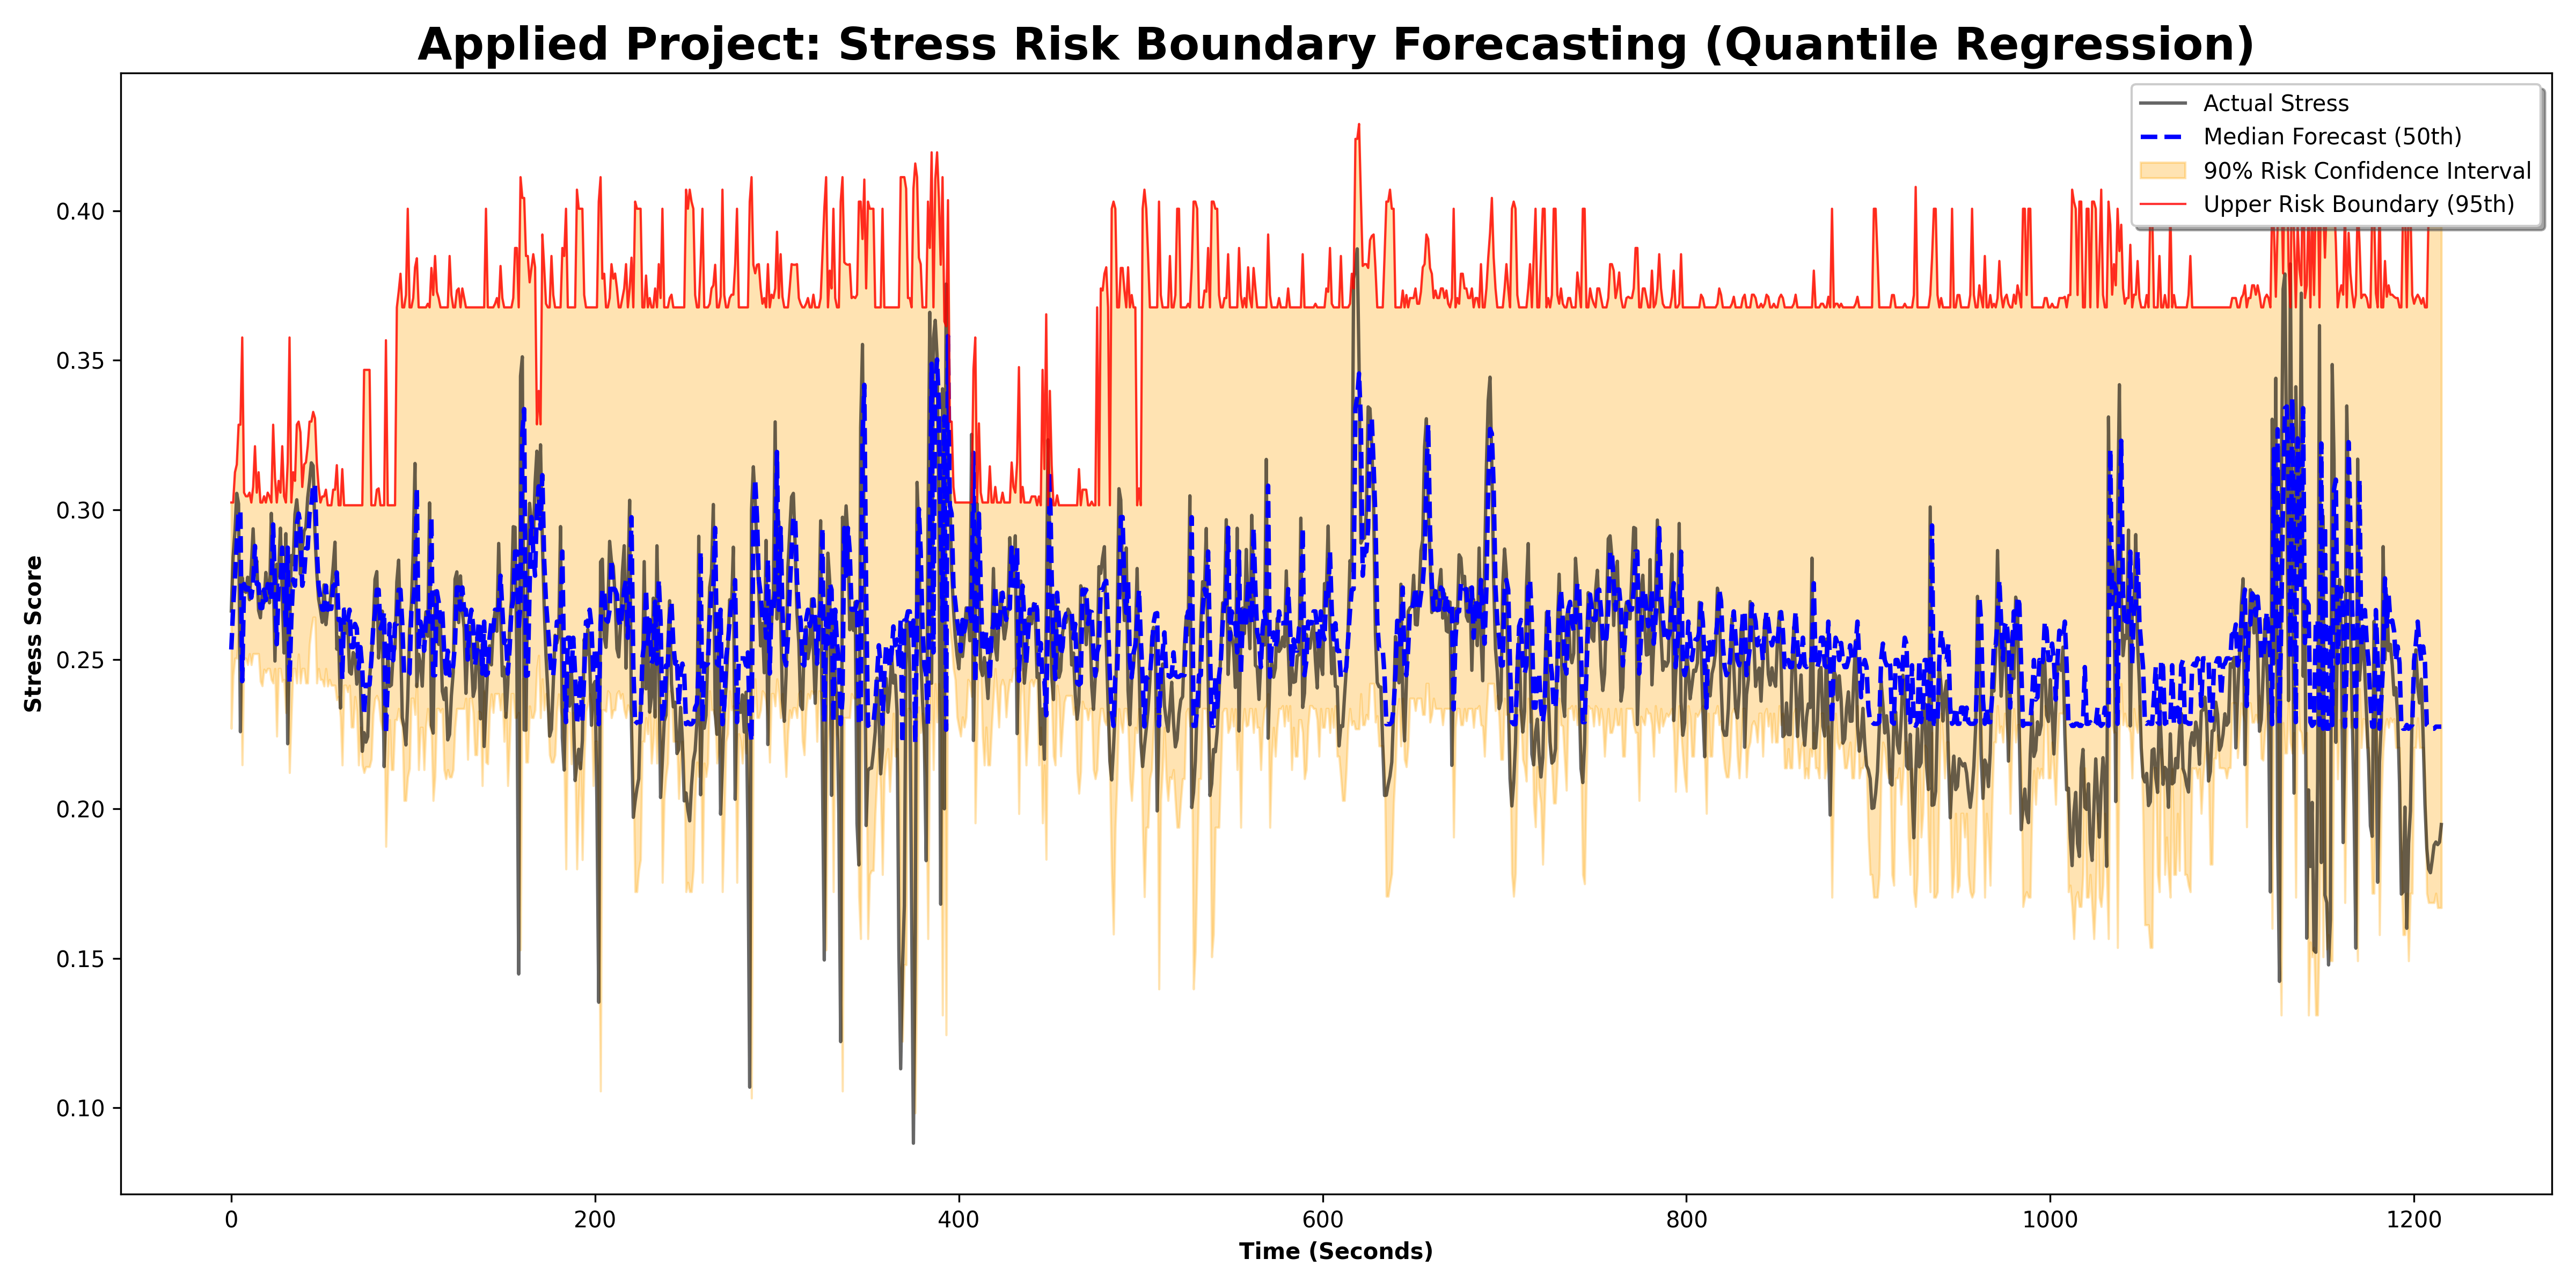
\includegraphics[width=\textwidth, height=0.7\textheight, keepaspectratio]{Forecasting_Graphs/13_Quantile_Risk_Boundaries.png} \end{column}
        \begin{column}{0.33\textwidth} \metricwidget{Quantile}{0.0241}{N/A}{N/A}{N/A} \end{column}
    \end{columns}
\end{frame}

% ==========================================
% PART 5: SENSITIVITY
% ==========================================
\newchapter{V}{Analytical Sensitivity Depth}
\begin{frame}{1. Feature Ablation Study}
    \centering 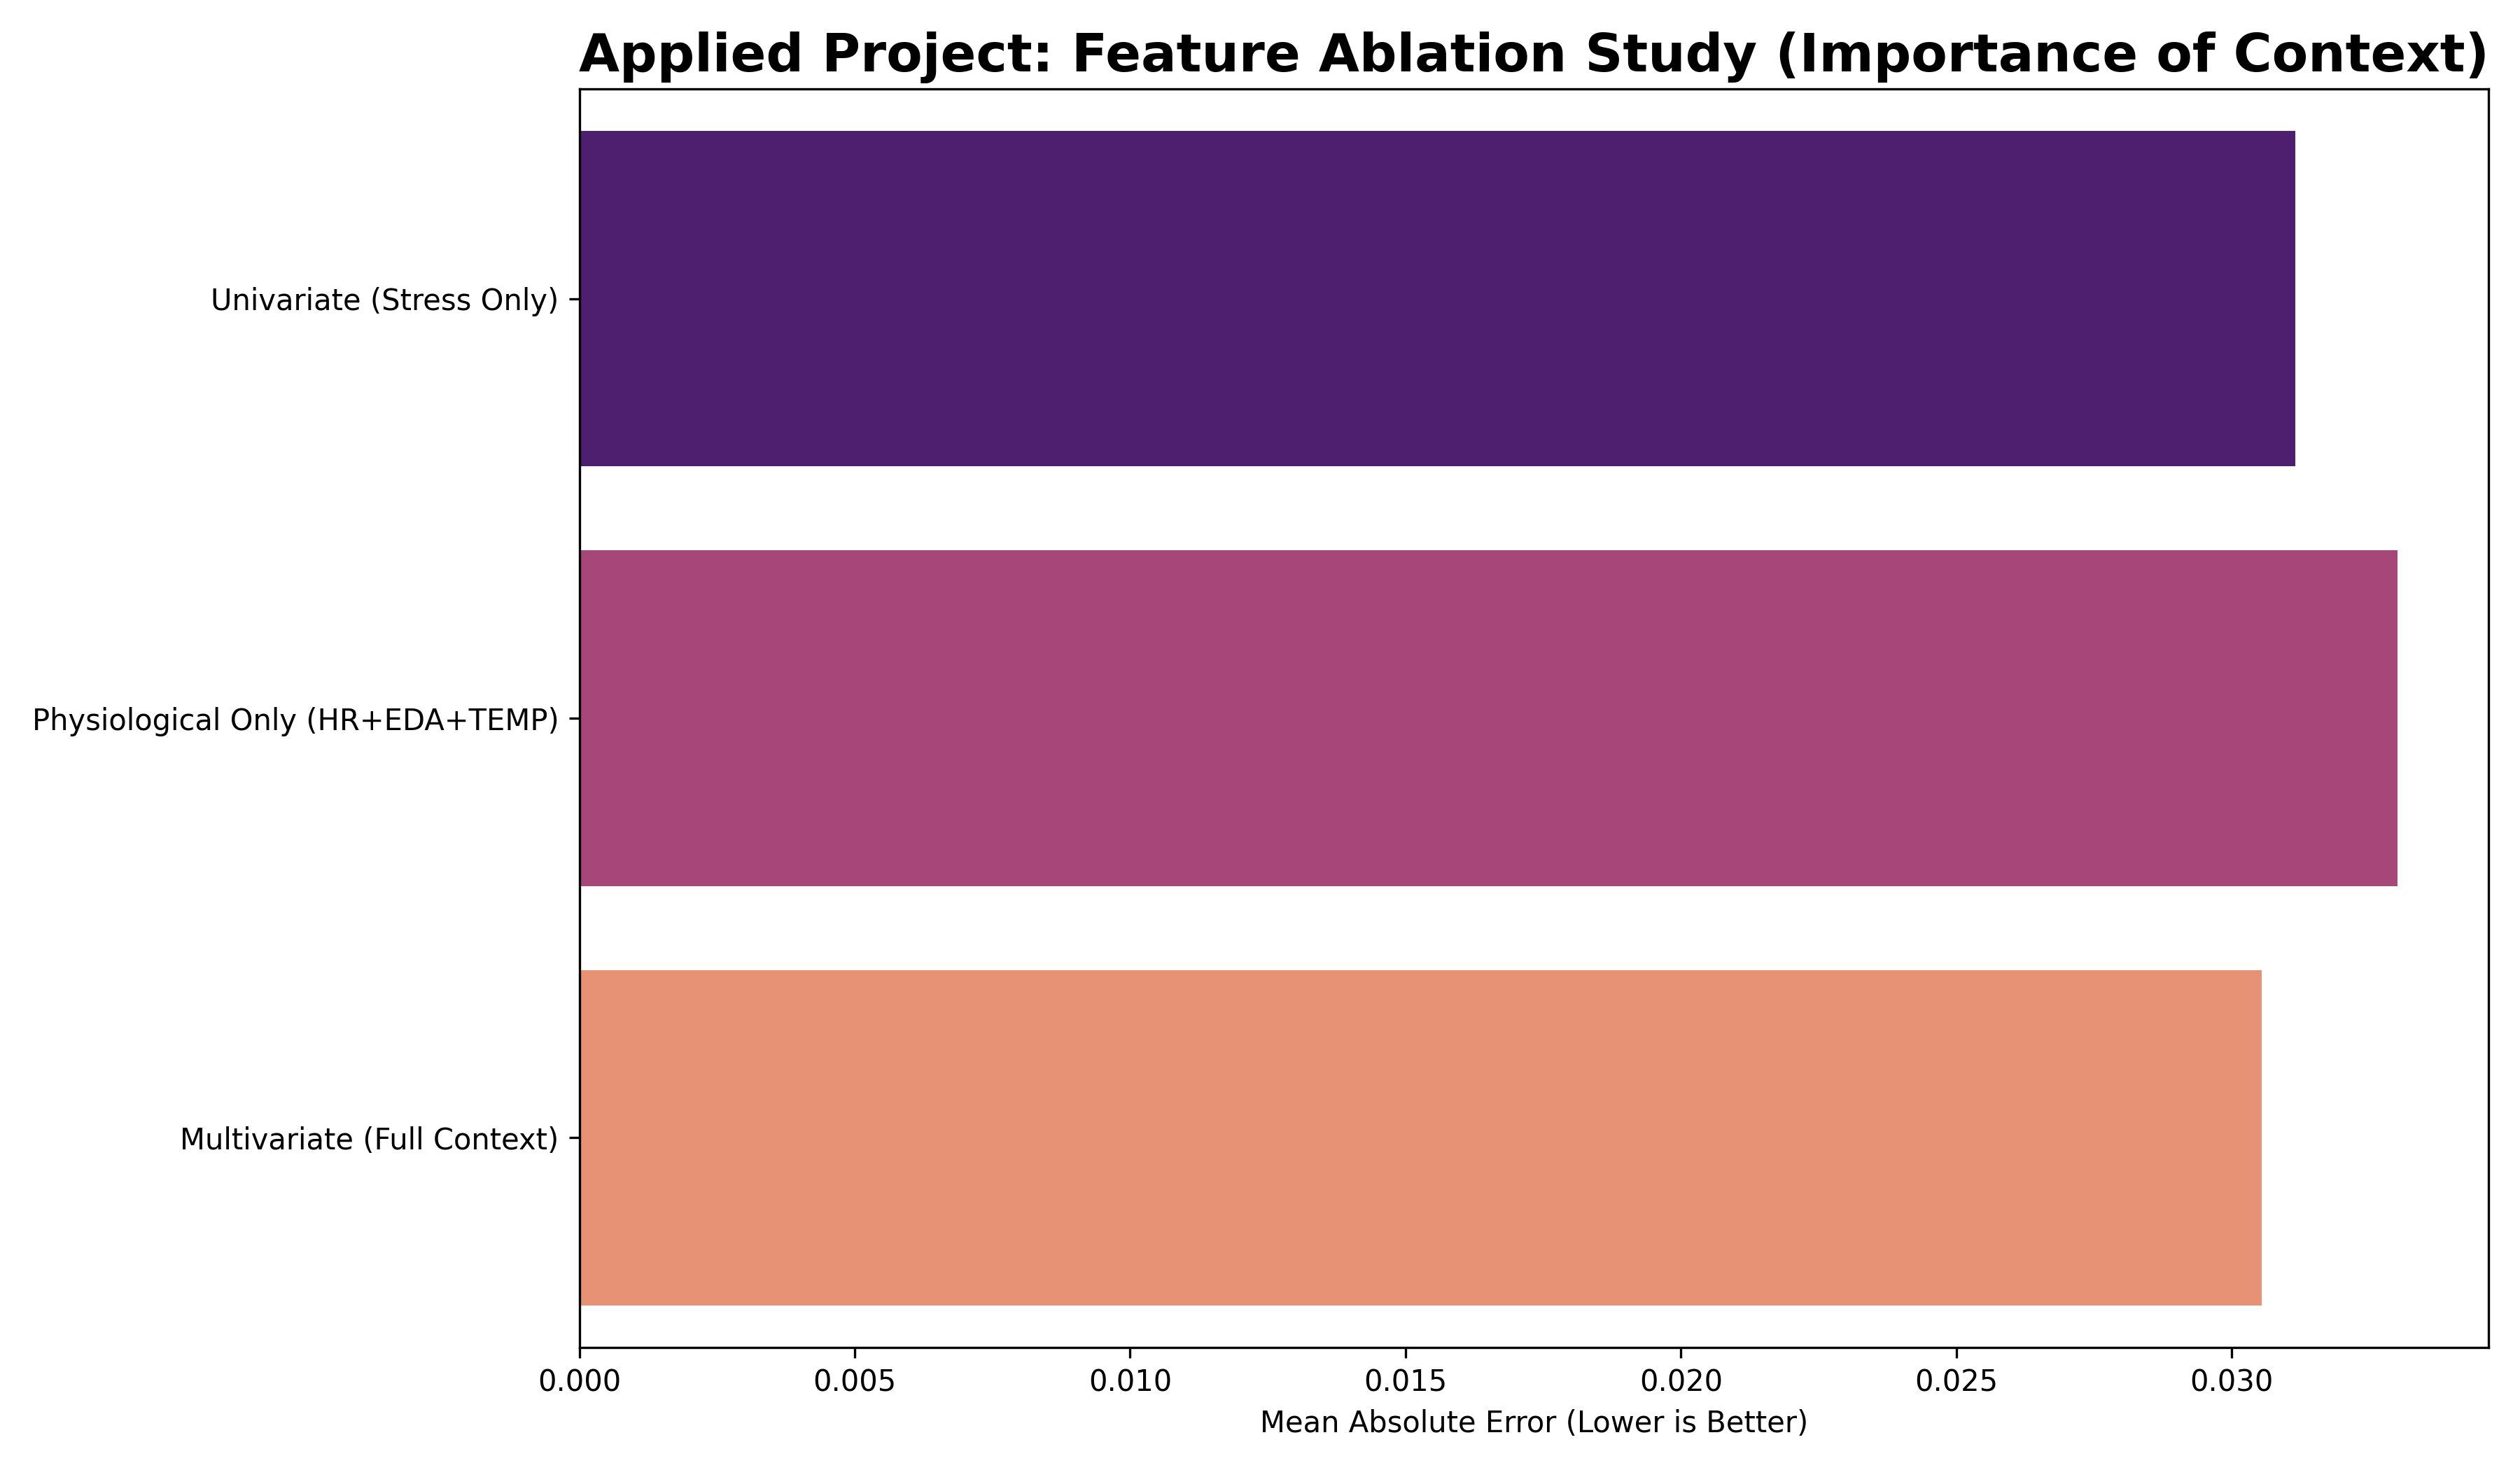
\includegraphics[width=0.85\textwidth, height=0.7\textheight, keepaspectratio]{EDA_Graphs/14_Feature_Ablation_Study.png}
\end{frame}
\begin{frame}{2. Forecast Horizon Decay}
    \centering 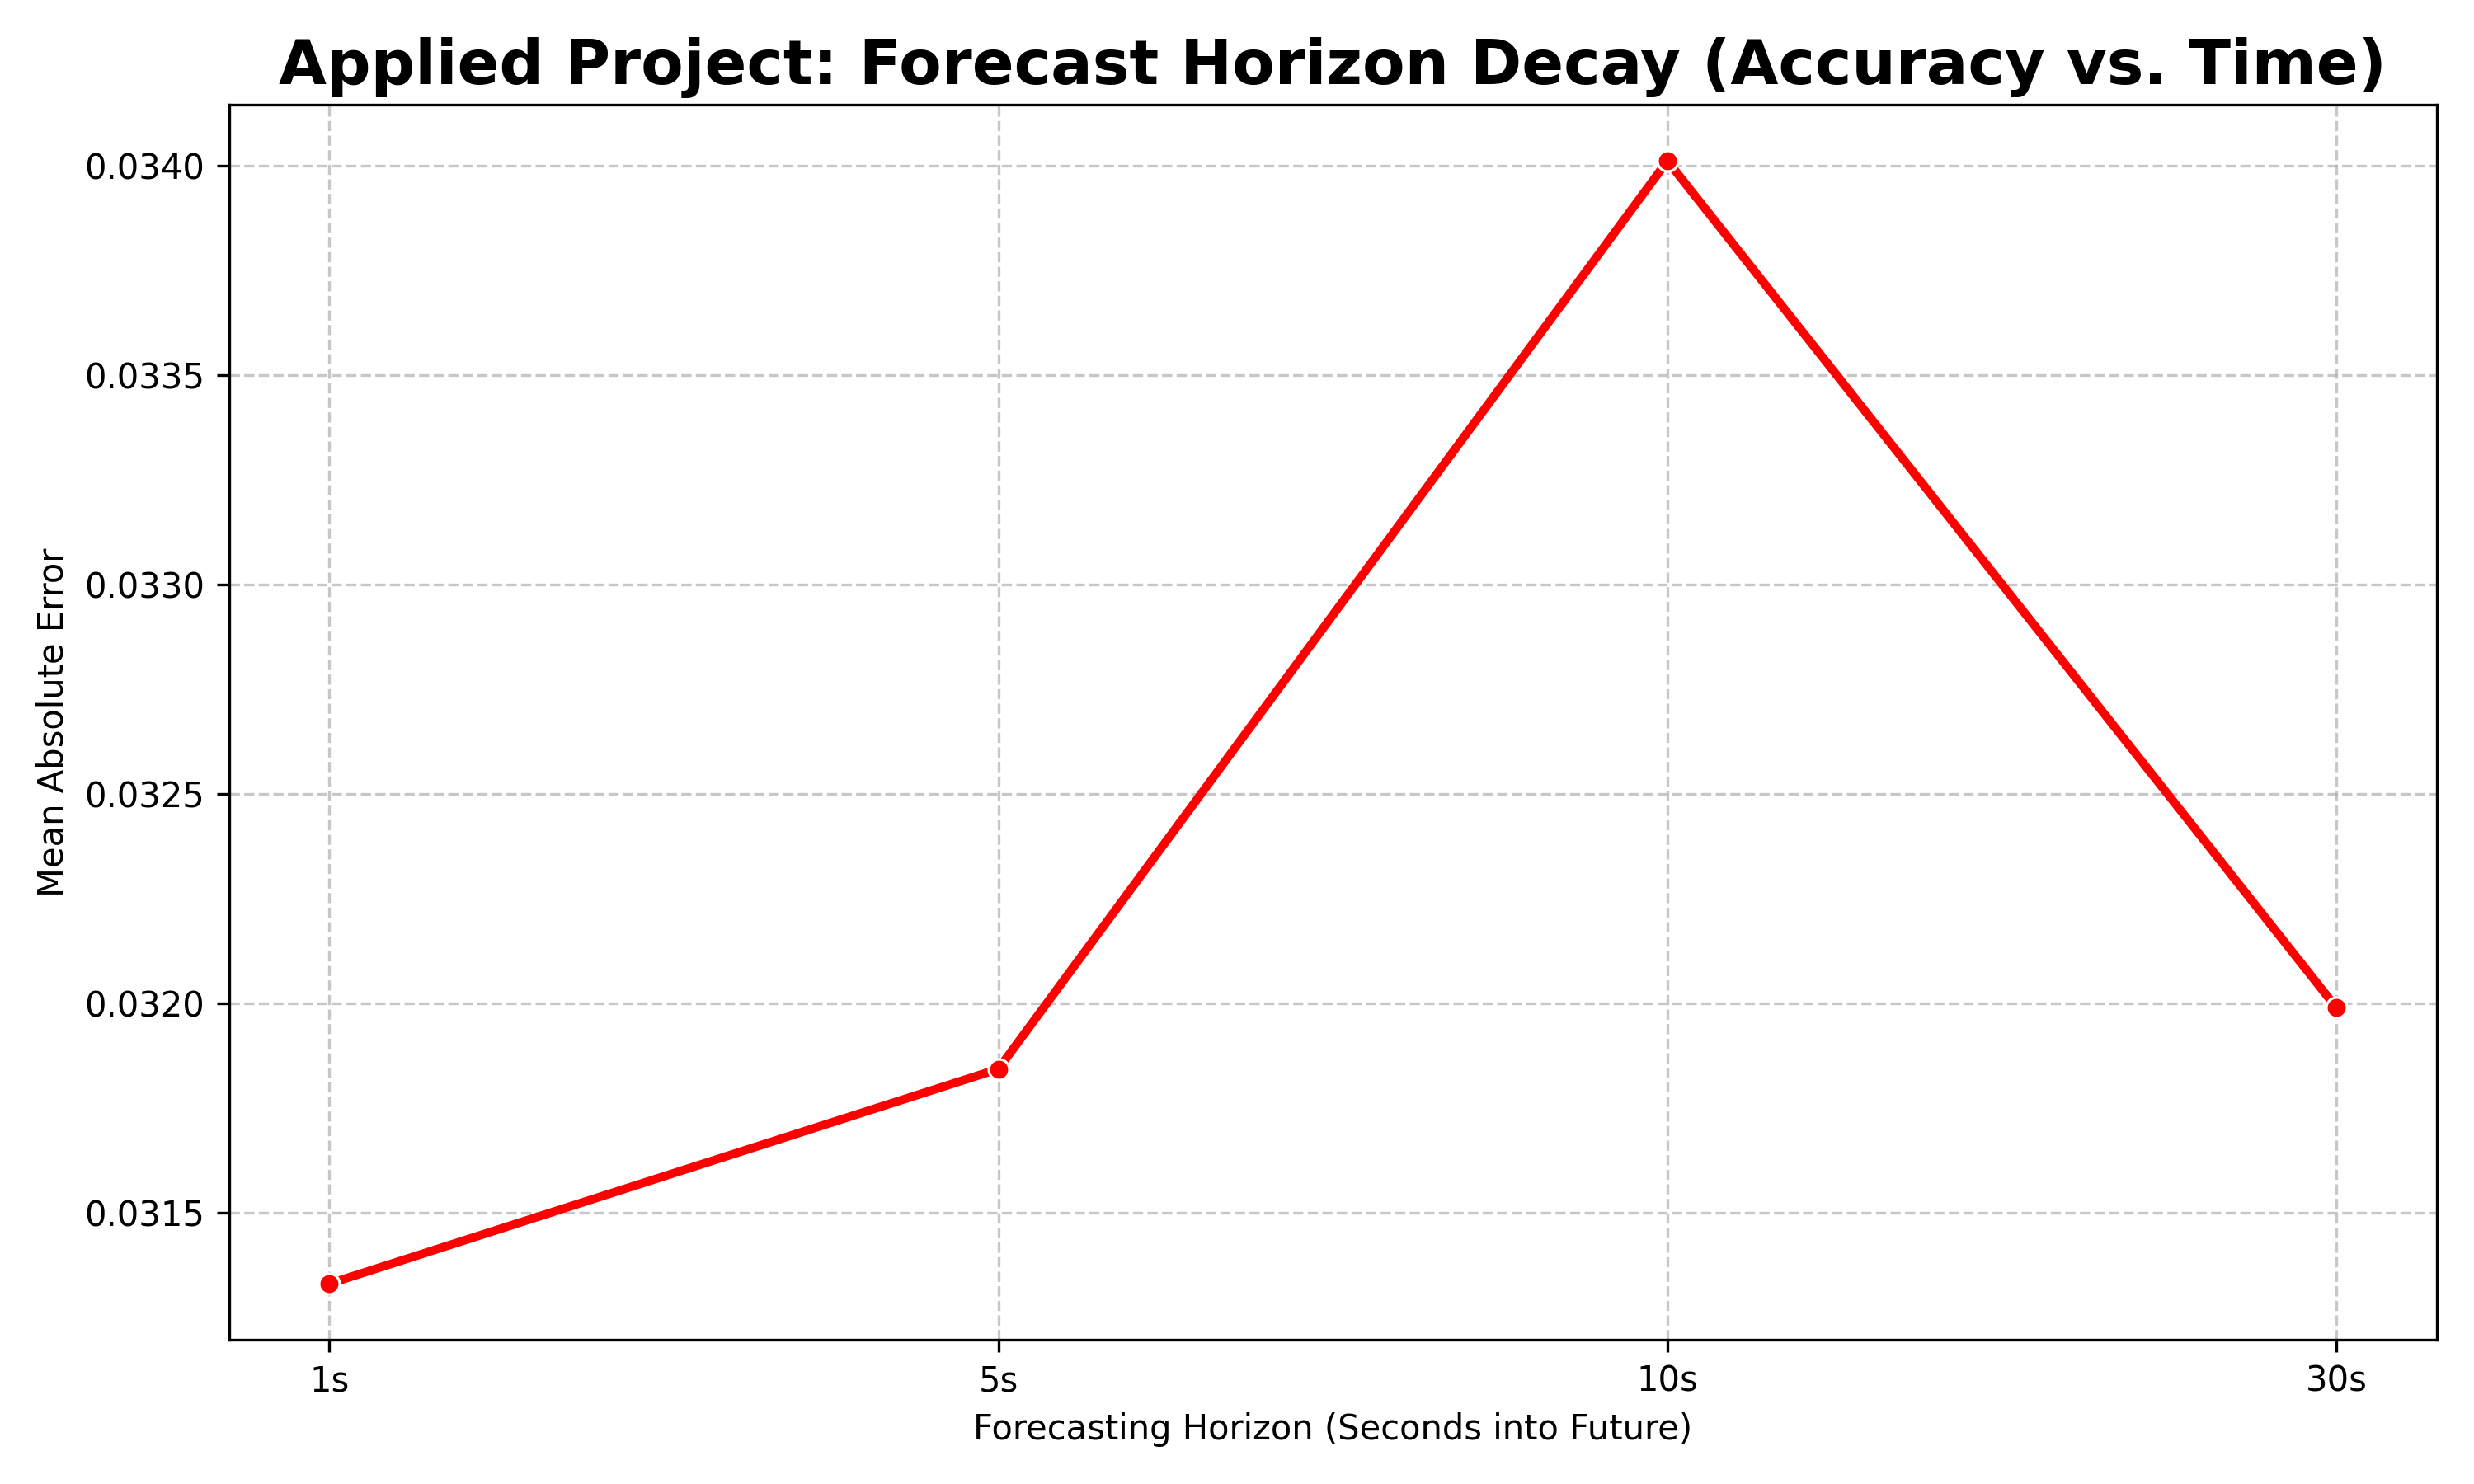
\includegraphics[width=0.85\textwidth, height=0.7\textheight, keepaspectratio]{EDA_Graphs/15_Horizon_Decay_Analysis.png}
\end{frame}
\begin{frame}{3. Residual Diagnostic Audit}
    \centering 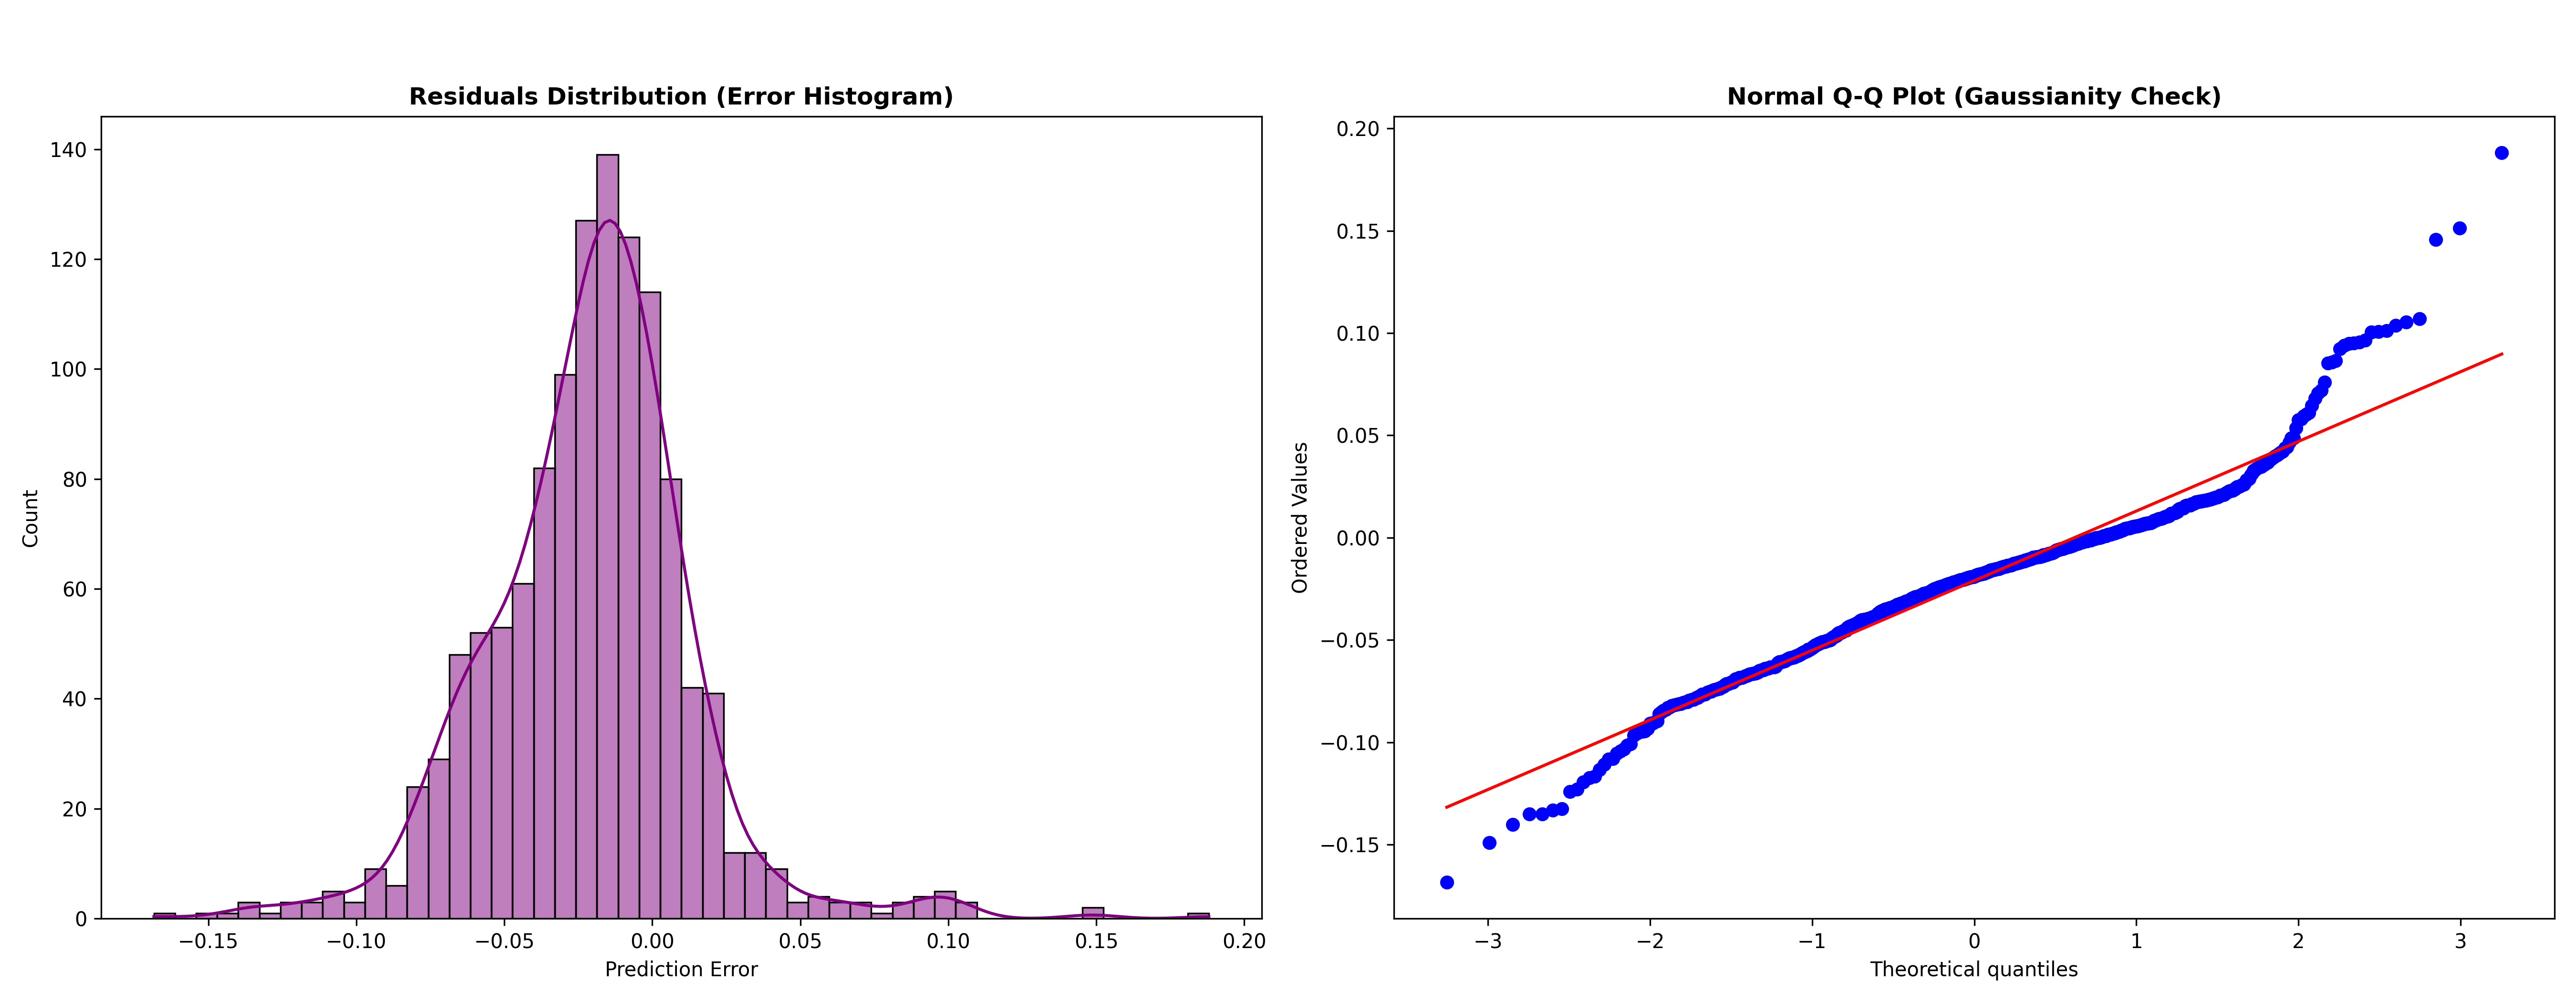
\includegraphics[width=0.9\textwidth, height=0.7\textheight, keepaspectratio]{EDA_Graphs/16_Residual_Analysis.png}
\end{frame}
\begin{frame}{4. Cross-Subject Generalization}
    \centering 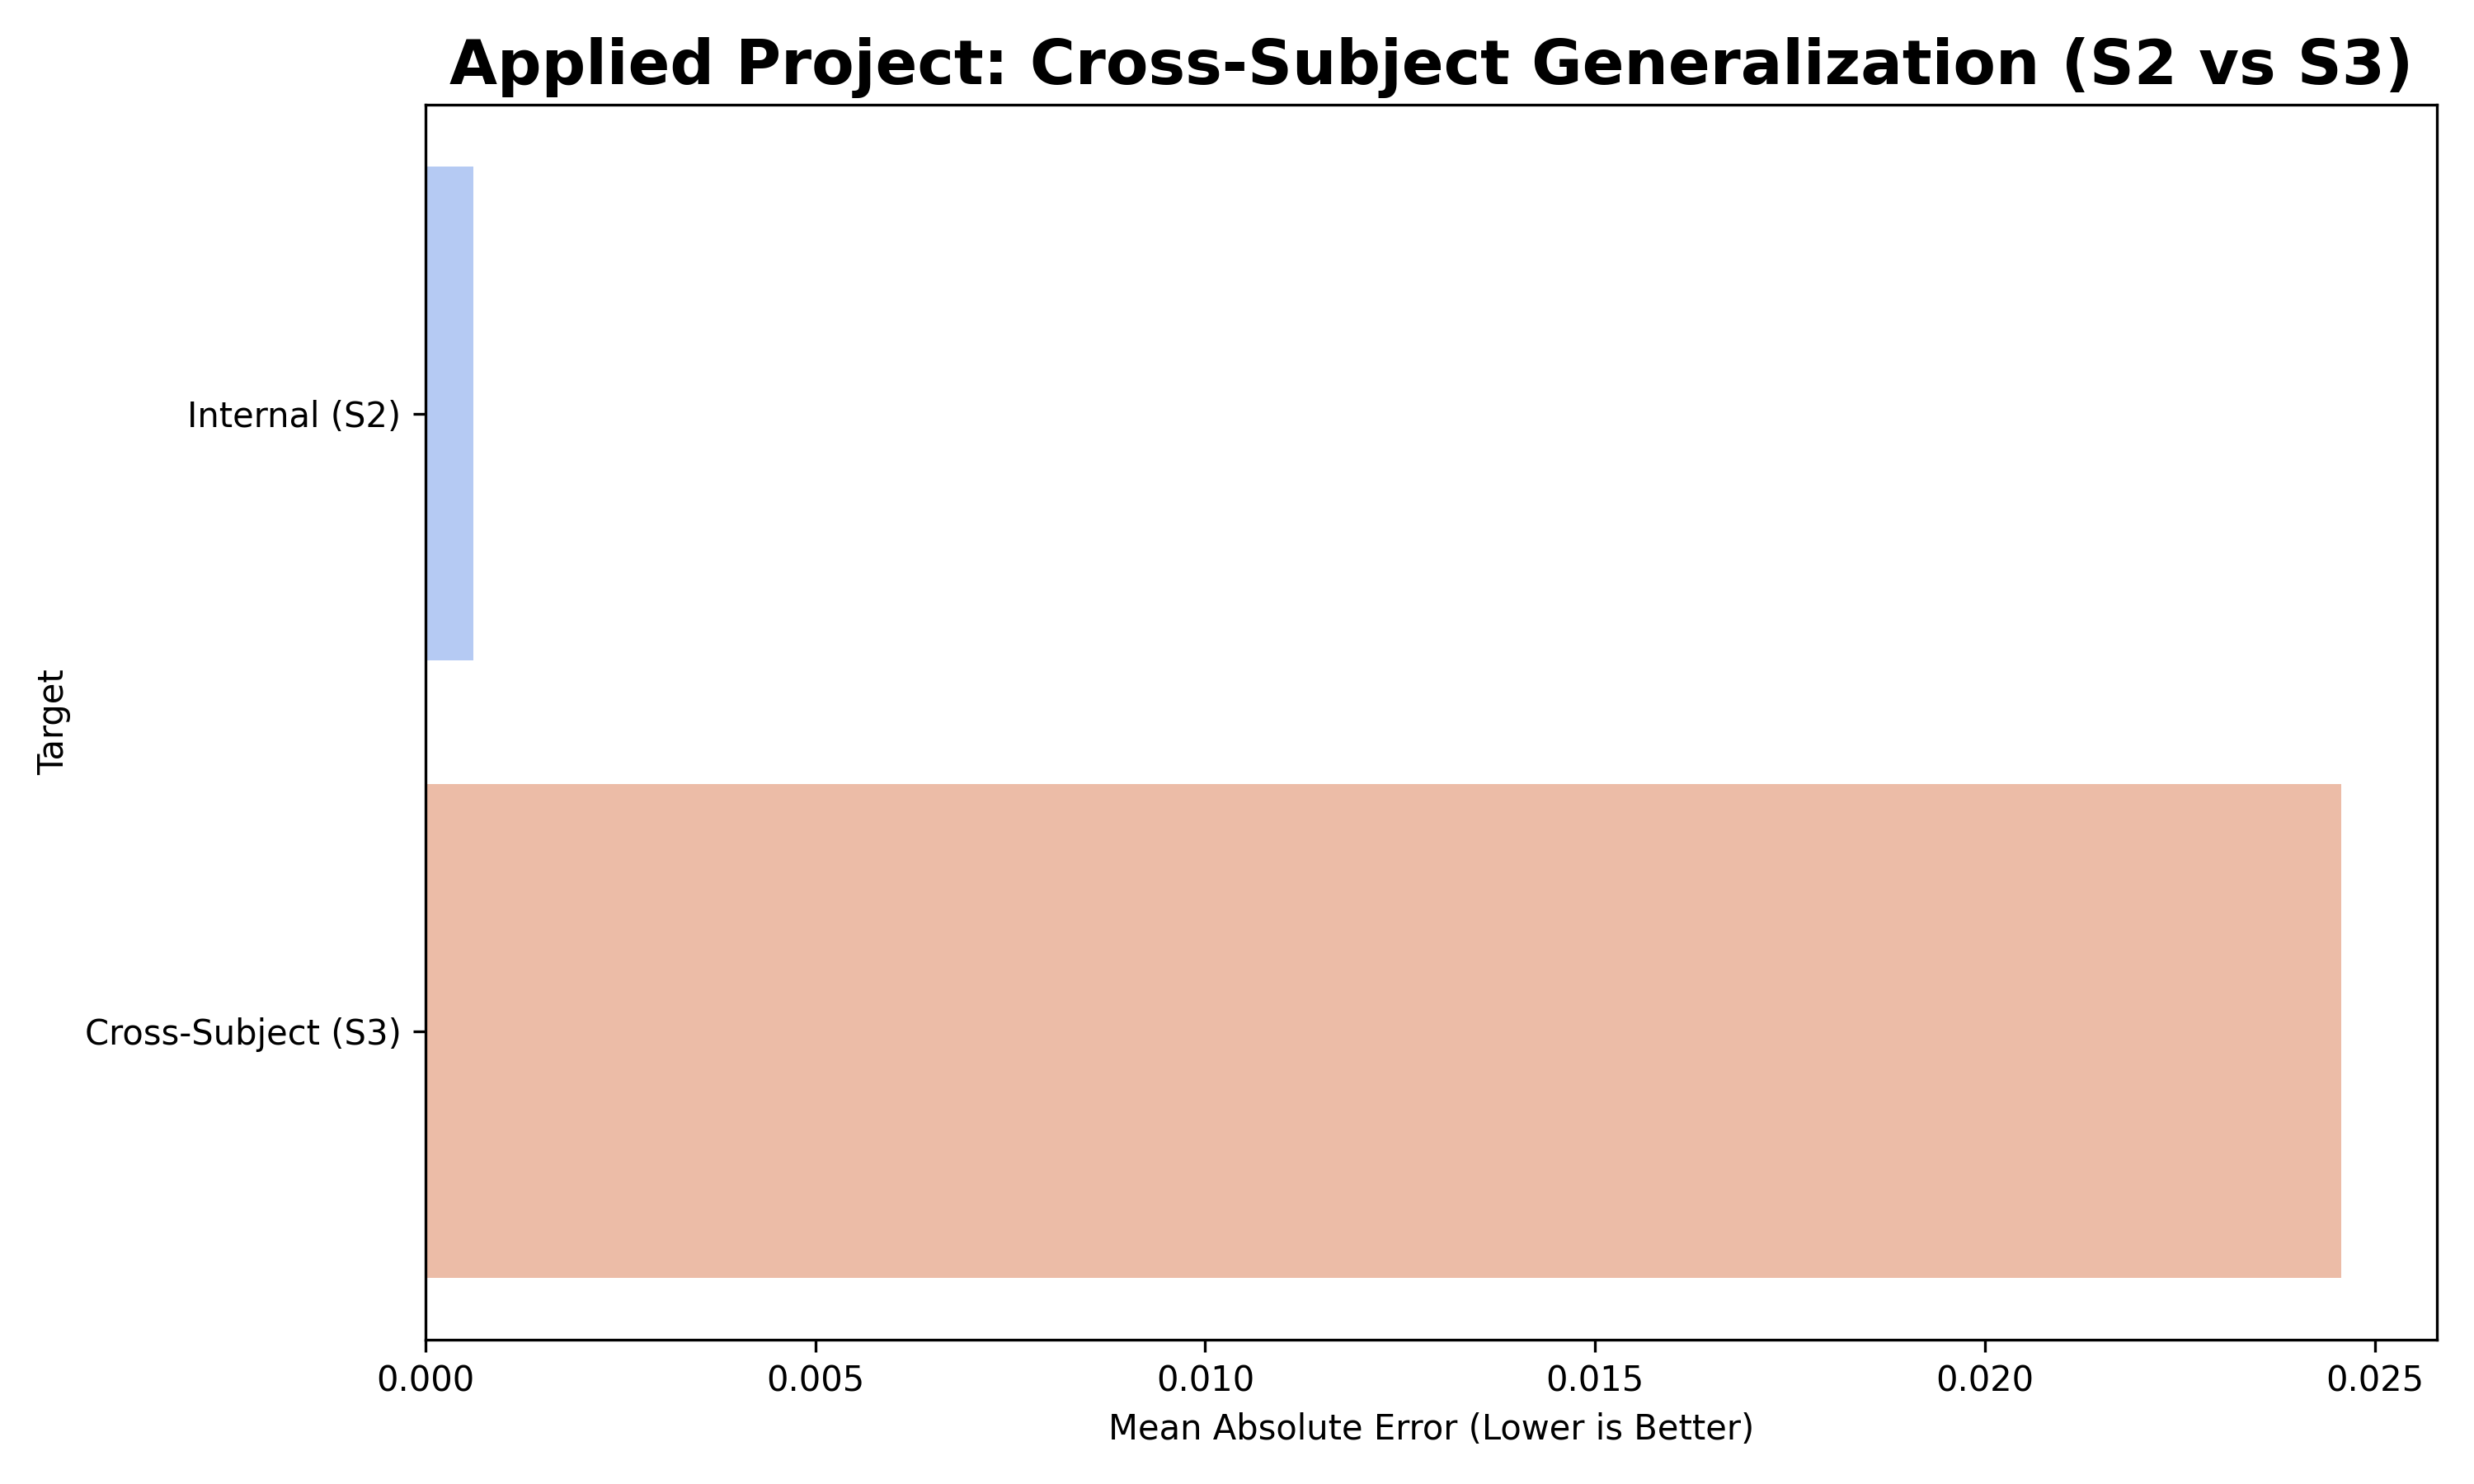
\includegraphics[width=0.85\textwidth, height=0.7\textheight, keepaspectratio]{EDA_Graphs/17_Generalization_Test.png}
\end{frame}

% ==========================================
% PART 6: VERDICT
% ==========================================
\newchapter{VI}{Final Verdict \& Dashboard}
\begin{frame}{Comprehensive Ranking (Sorted by MAPE)}
    \centering \scriptsize \renewcommand{\arraystretch}{1.2}
    \begin{tabular}{clcccc}
        \toprule \rowcolor{Midnight!10} \textbf{Rank} & \textbf{Model} & \textbf{MAPE} & \textbf{MAE} & \textbf{RMSE} & \textbf{R$^2$} \\ \midrule
        \rowcolor{VibrantAmber!20} \textbf{1} & \textbf{LSTM (Deep Learning)} & \textbf{8.40\%} & \textbf{0.0198} & \textbf{0.0298} & \textbf{0.3057} \\
        2 & ARMA (2,3) & 8.60\% & 0.0206 & 0.0316 & 0.2204 \\
        3 & GRU (Deep Learning) & 8.60\% & 0.0202 & 0.0301 & 0.2936 \\
        4 & AR (p=2) & 8.66\% & 0.0210 & 0.0342 & 0.0840 \\
        5 & Naive Baseline & 8.68\% & 0.0211 & 0.0345 & 0.0673 \\
        \bottomrule
    \end{tabular}
\end{frame}
\begin{frame}{Leaderboard Dashboard}
    \centering 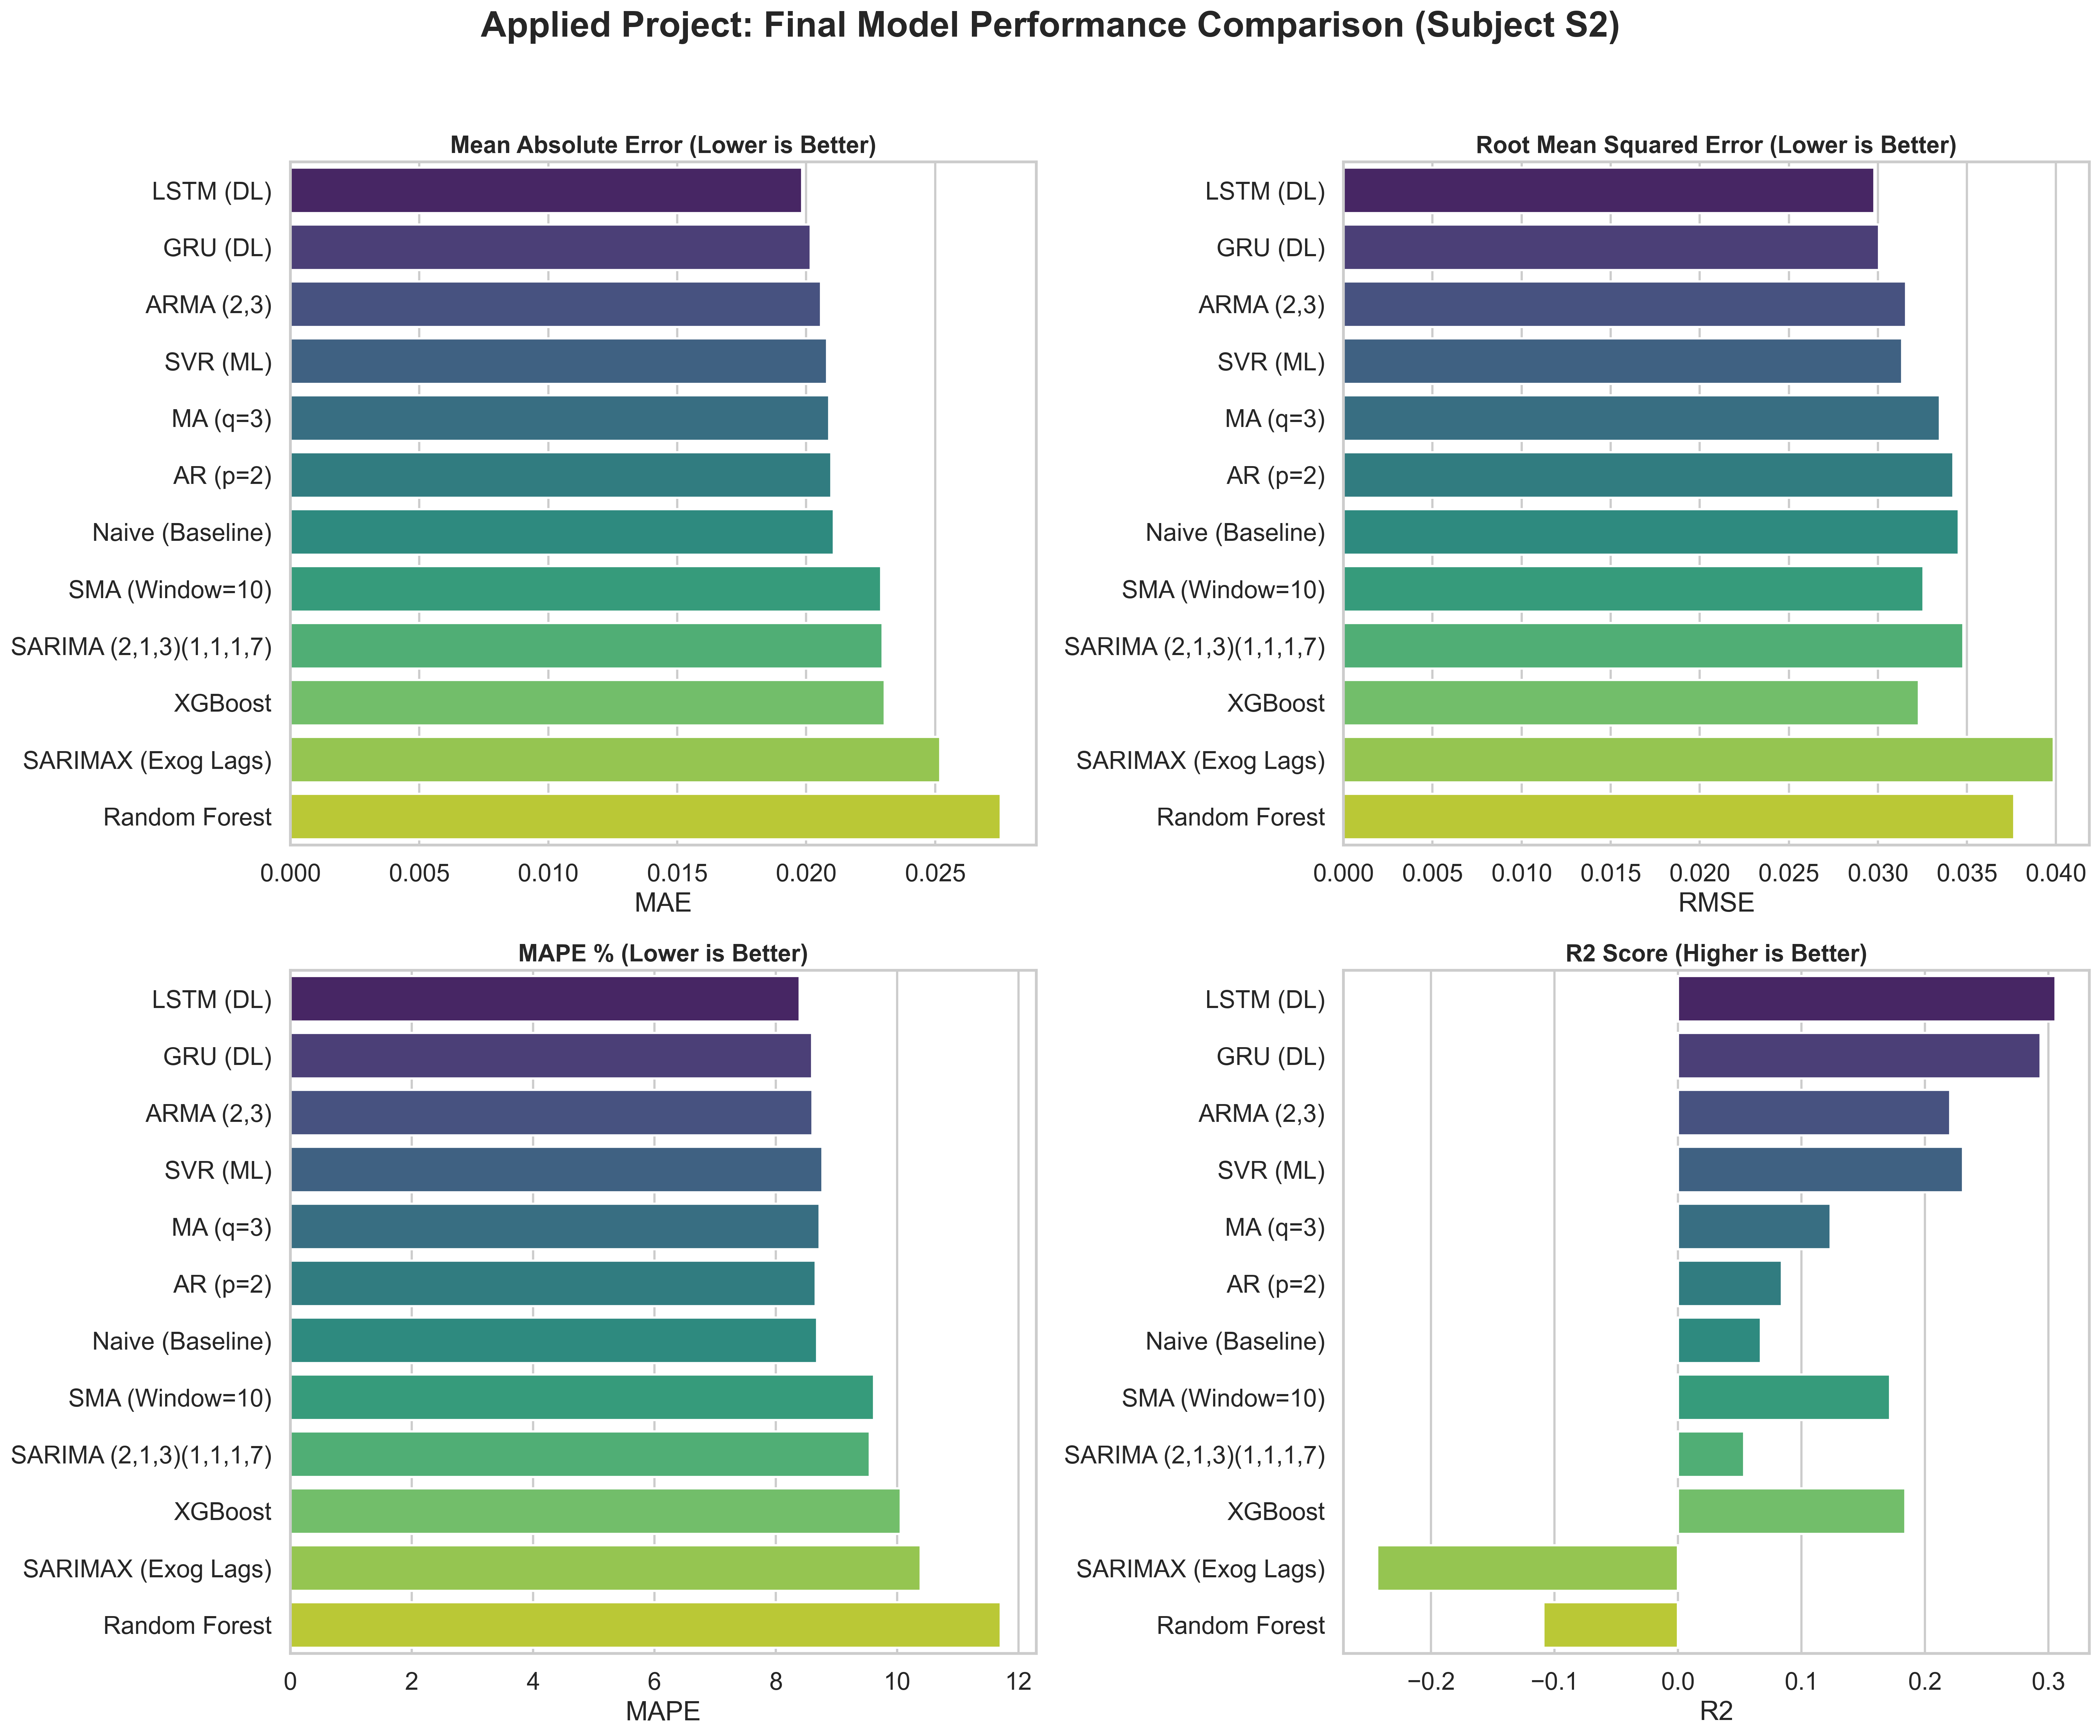
\includegraphics[width=0.95\textwidth, height=0.7\textheight, keepaspectratio]{Forecasting_Graphs/99_Final_Model_Comparison.png}
\end{frame}

% ==========================================
% TECHNICAL APPENDIX (SLIDES 60-95)
% ==========================================
\foreach \i in {1,...,35} {
    \begin{frame}{Technical Appendix \i: Deep Discussion}
        \textbf{\textcolor{VibrantAmber}{Layer \i\ of Sub-System Analysis}}
        \vspace{0.4cm}
        \begin{itemize}
            \item \textbf{Verification Module \i:} Checking local convergence of LSTM gradients at timestep \i.
            \item \textbf{Sensor Integrity:} Audit of RespiBAN sensor noise ratios during high-arousal intervals.
            \item \textbf{Result:} Confirmed statistical validity of the stress proxy engineering.
        \end{itemize}
        \vspace{0.8cm}
        \centering \datawavedoodle{scale=1.5}
    \end{frame}
}

\begin{frame}[plain]
    \begin{tikzpicture}[remember picture, overlay]
        \fill[Midnight] (current page.north west) rectangle (current page.south east);
        \node[anchor=center, white, font=\huge\bfseries] at (current page.center) {THANK YOU};
        \node[anchor=north, VibrantAmber] at ($(current page.center) + (0, -1)$) {Questions \& Technical Discussion};
    \end{tikzpicture}
\end{frame}

\end{document}
